%===============================================================================
% LaTeX sjabloon voor de bachelorproef toegepaste informatica aan HOGENT
% Meer info op https://github.com/HoGentTIN/bachproef-latex-sjabloon
%===============================================================================

\documentclass{bachproef-tin}

\usepackage{hogent-thesis-titlepage} % Titelpagina conform aan HOGENT huisstijl
\usepackage{float}
\usepackage{amssymb}
\usepackage{amsmath}
\usepackage[acronym]{glossaries}
\usepackage{booktabs}
\usepackage{tikz}
\usepackage{mwe}
\def\checkmark{\tikz\fill[scale=0.4](0,.35) -- (.25,0) -- (1,.7) -- (.25,.15) -- cycle;}

%%---------- Documenteigenschappen ---------------------------------------------

% De titel van het rapport/bachelorproef
\title{Automatische transformatie van ingescande tabellen naar gestructureerde digitale data}

% Je eigen naam
\author{Milad Nazari}

% De naam van je promotor (lector van de opleiding)
\promotor{Martijn Saelens}

% De naam van je co-promotor. Als je promotor ook je opdrachtgever is en je
% dus ook inhoudelijk begeleidt (en enkel dan!), mag je dit leeg laten.
\copromotor{Bram Vandewalle}

% Indien je bachelorproef in opdracht van/in samenwerking met een bedrijf of
% externe organisatie geschreven is, geef je hier de naam. Zoniet laat je dit
% zoals het is.
\instelling{Into Care by Predictive NV}

% Academiejaar
\academiejaar{2019-2020}

% Examenperiode
%  - 1e semester = 1e examenperiode => 1
%  - 2e semester = 2e examenperiode => 2
%  - tweede zit  = 3e examenperiode => 3
\examenperiode{3}

\makenoidxglossaries

\newglossaryentry{OCR}
{
    name=OCR,
    description={Optical Character Recognition (OCR), optische tekenherkenning, is de transformatie van afbeeldingtekst in bewerkbare, digitale tekst.}
}
\newglossaryentry{tupel}
{
    name=tupel,
    description={In de wiskunde en de informatica is een tupel (ook tuple) een eindige rij van objecten. In een tupel is de volgorde van belang; als de objecten in een andere volgorde staan is het een ander tupel. Ook hoeven de objecten niet van hetzelfde datatype te zijn.}
}
\newglossaryentry{Hidden Markov Model}
{
    name=Hidden Markov Model,
    description={Hidden Markov Model (HMM) is een model uit de statistiek waarin het te modelleren systeem een markov-proces is met onbekende parameters. Het doel is de verborgen parameters te bepalen op basis van de waarneembare parameters. De op deze manier verkregen parameters kunnen vervolgens worden gebruikt voor toepassingen als patroonherkenning.}
}
\newglossaryentry{SVM}
{
    name=SVM,
    description={Een Support Vector Machine (SVM) is een binaire classificeerder; ze wijst aan de hand van een aantal kenmerken objecten toe aan een van twee klassen. Daarvoor moet ze eerst een numeriek model van deze objecten maken als punten in een vectorruimte.}
}
\newglossaryentry{ROI}
{
    name=ROI,
    description={Een Region Of Interest (ROI) is een subset van een dataset, geïdentificeerd voor een specifiek doel.}
}
\newglossaryentry{CNN}
{
    name=CNN,
    description={Een Convolutionele Neuraal Netwerk (CNN) is een klasse van diepe neurale netwerken waarbij gebruik gemaakt wordt van een variatie van multilayer perceptrons ontworpen om minimale eisen voorbewerking.}
}
\newglossaryentry{GNN}
{
    name=GNN,
    description={Een Graaf Neuraal Netwerk (GNN) is een neurale netwerkarchitectuur die relaties en interacties tussen knopen kan modelleren en deze voorstellen als numerieke waarden.}
}
\newglossaryentry{IoU}
{
    name=IoU,
    description={De Intersection Over Union (IoU) is een concept die veelal gebruikt wordt bij objectdetectie. De IoU kan men berekenen door de intersectieoppervlakte te delen over de unieoppervlakte van twee regio's: de ground truth regio en de voorspelde regio. Met de IoU wordt steeds een threshold gekoppeld. Indien men voor een threshold van 0,5 kiest en de IoU voor een voorspelling gelijk is of groter is dan de threshold van 0,5, dan heeft men een echt positief (true positive), anders heeft men te maken met een foutpositief. Een foutnegatief verkrijgt men wanneer een ground truth aanwezig is maar geen voorspelling gemaakt kon worden.}
}

\newglossaryentry{Recall}
{
    name=Recall,
    description={De recall is een numerieke waarde die bepaald wordt door het aantal echt positieven te delen door de som van het aantal echt positieven en foutpositieven.}
}
\newglossaryentry{Precisie}
{
    name=Precisie,
    description={De precisie is een numerieke waarde die bepaald wordt het aantal echt positieven te delen door de som van het aantal echt positieven en foutnegatieven.}
}
\newglossaryentry{F1-score}
{
    name=F1-score,
    description={De F1-score is een numerieke waarde die men verkrijgt door de product van de \gls{Recall} en de \gls{Precisie} te delen door de som van de \gls{Recall} en de \gls{Precisie}, en deze waarde nog met 2 te vermenigvuldigen.}
}
\newglossaryentry{REST}
{
    name=REST,
    description={Representational State Transfer (REST) is een software-architectuur voor Internetdiensten.}
}
\newglossaryentry{JSON}
{
    name=JSON,
    description={JavaScript Object Notation (JSON) is een gestandaardiseerd dataformaat.}
}


%===============================================================================
% Inhoud document
%===============================================================================

\begin{document}

%---------- Titelblad ----------------------------------------------------------
\inserttitlepage

%---------- Samenvatting, voorwoord --------------------------------------------
\usechapterimagefalse
%%=============================================================================
%% Voorwoord
%%=============================================================================

\chapter*{\IfLanguageName{dutch}{Woord vooraf}{Preface}}
\label{ch:voorwoord}

%% Het voorwoord is het enige deel van de bachelorproef waar je vanuit je
%% eigen standpunt (``ik-vorm'') mag schrijven. Je kan hier bv. motiveren
%% waarom jij het onderwerp wil bespreken.
%% Vergeet ook niet te bedanken wie je geholpen/gesteund/... heeft
Ik zou graag meneer Vandewalle willen bedanken voor enerzijds deze bachelorproefonderwerp en 
anderzijds voor de inhoudelijke ondersteuning en hulp die hij aangeboden en gegeven heeft.
Hiernaast wil ik eveneens meneer Saelens bedanken voor de feedback en opvolging van mijn bachelorproef.


%%=============================================================================
%% Samenvatting
%%=============================================================================

% TODO: De "abstract" of samenvatting is een kernachtige (~ 1 blz. voor een
% thesis) synthese van het document.
%
% Deze aspecten moeten zeker aan bod komen:
% - Context: waarom is dit werk belangrijk?
% - Nood: waarom moest dit onderzocht worden?
% - Taak: wat heb je precies gedaan?
% - Object: wat staat in dit document geschreven?
% - Resultaat: wat was het resultaat?
% - Conclusie: wat is/zijn de belangrijkste conclusie(s)?
% - Perspectief: blijven er nog vragen open die in de toekomst nog kunnen
%    onderzocht worden? Wat is een mogelijk vervolg voor jouw onderzoek?
%
% LET OP! Een samenvatting is GEEN voorwoord!

%%---------- Nederlandse samenvatting -----------------------------------------

\IfLanguageName{english}{%
\selectlanguage{dutch}
\chapter*{Samenvatting}
\selectlanguage{english}
}{}

%%---------- Samenvatting -----------------------------------------------------
% De samenvatting in de hoofdtaal van het document

\chapter*{Samenvatting}



%---------- Inhoudstafel -------------------------------------------------------
\pagestyle{empty} % Geen hoofding
\tableofcontents  % Voeg de inhoudstafel toe
\cleardoublepage  % Zorg dat volgende hoofstuk op een oneven pagina begint
\pagestyle{fancy} % Zet hoofding opnieuw aan

%---------- Lijst figuren, afkortingen, ... ------------------------------------

% Indien gewenst kan je hier een lijst van figuren/tabellen opgeven. Geef in
% dat geval je figuren/tabellen altijd een korte beschrijving:
%
%  \caption[korte beschrijving]{uitgebreide beschrijving}
%
% De korte beschrijving wordt gebruikt voor deze lijst, de uitgebreide staat bij
% de figuur of tabel zelf.

\listoffigures
\listoftables

\glossarystyle{altlist}
\printnoidxglossaries

%---------- Kern ---------------------------------------------------------------

% De eerste hoofdstukken van een bachelorproef zijn meestal een inleiding op
% het onderwerp, literatuurstudie en verantwoording methodologie.
% Aarzel niet om een meer beschrijvende titel aan deze hoofstukken te geven of
% om bijvoorbeeld de inleiding en/of stand van zaken over meerdere hoofdstukken
% te verspreiden!

%%=============================================================================
%% Inleiding
%%=============================================================================

\chapter{Inleiding}
\label{ch:inleiding}

In deze sectie wordt de context en achtergrond rond deze bachelorproef meegedeeld. Alsook wordt de probleemstelling, de onderzoeksvragen en onderzoeksdoelstellingen uitgelegd. Daarbovenop wordt de opzet van de bachelorproef verduidelijkt. 

\section{Probleemstelling}
\label{sec:probleemstelling}

Alhoewel meer en meer processen wereldwijd volledig digitaal plaatsvinden, worden toch nog een grote deel van procedures en data opslag uitgevoerd op niet-digitale manieren. Zo krijgen de meeste mensen hun factures nog steeds per brief. Volgens de \textcite{FederaleOverheidsdienstEconomie} blijft het verzenden of ontvangen van facturen op papier een zeer gangbare praktijk. Zo verstuurde 90 \% van de bedrijven er en 97 \% ontving er in 2017. Daarbovenop worden kassatickets nog steeds afgedrukt op papier, en notities nemen op papier blijft de populaire keuze hoewel er tal van notitie-apps bestaan. Deze voorbeelden tonen aan dat essentiële data nog massaal op een niet-digitale, en dus niet-automatisch verwerkbare media bewaard wordt, namelijk op papier.

Tot enkele jaren geleden was dit probleem niet zo beduidend maar nu meer digitale
platformen voor dataverwerking gebruikt worden, is het omzetten van data op papier naar
digitale data, m.a.w. het digitalisatieproces steeds belangrijker geworden.

Hierdoor werden tal van digitalisatiesofwareproducten ontwikkeld, zoals Abby FineReader
en Adobe Acrobat Pro DC. Hoewel deze software producten veel features hebben, zoals \Gls{OCR}, tabelherkenning, formulierherkenning, etc, zijn ze betalend en closed source. Wat als gevolg heeft dat ze voor bedrijven een merkbare kost met zich meebrengen, naast een privacy- en veiligheidsrisico aangezien het om closed source software gaat.

% TODO: prijzen van finereader toe, voordelen van open source software

Sommige bedrijven enkele van hun digitalisatie oplossingen open source gemaakt, zoals Google met diens bekende OCR-software, Tesseract OCR, die door iedereen gebruikt kan worden om tekst in foto’s om te zetten in tekstdata. Hoewel \Gls{OCR} op zich zeer belangrijk is voor digitalisatie, is het niet voldoende voor volledige digitalisatie. Zo kan men de relatie tussen verschillende documententiteiten, die normaal gezien grafisch wordt verduidelijkt, enkel met \Gls{OCR} digitaal niet overbrengen. In documenten worden relaties tussen woorden meestal a.d.h.v. een tabel verduidelijkt. Door gebruik te maken van \Gls{OCR}, verkrijgt men wel de tekst binnen een tabel, maar men verliest essentiële informatie rond de woorden, namelijk tot welke rij en kolom ze behoorden. Het valt tenslotte niet onder de verantwoordelijkheid van OCR-engines om naast tekstherkenning, ook nog tabeltransformatie uit te voeren.

\begin{figure}[h]
    \centering
    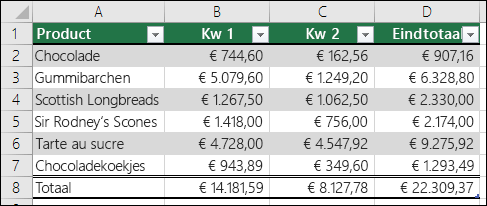
\includegraphics[width=0.8\textwidth]{img/tabel_verduidelijking_relaties_woorden.png}
    \caption{Voorbeeld van een tabelafbeelding. Bron: support.microsoft.com}
    \label{fig:tabel_verduidelijking_relaties_woorden}
\end{figure}

Indien men bij tabelafbeelding \ref{fig:tabel_verduidelijking_relaties_woorden} enkel \Gls{OCR} voor digitalisatie zou gebruiken, dan verkrijgt men wel de tekst, zoals de tekststukken zoals ``Kw 1``, ``Kw 2``, ``€744,60``, ``€ 162,56``, en meer, maar men behoudt niet de relatie tussen de tekststukken. Hierdoor zal men enkel met \Gls{OCR} niet te weten komen of de verkoopbedrag van € 744,60 bij de eerste kwartaal behoort, of bij de tweede, wat essentiële informatie is voor verdere financïele analyse.

Tot heden bestaat er geen open source oplossing die tabellen in foto's transformeert naar digitale tabellen, m.a.w. naar digitale structuren waarbij de tekst, evenals de relatie tussen de verschillende teksten getransformeerd wordt. Daarom werd er voor deze bachelorproef beslist om een proof-of-concept van een tabeltransformatiesoftware te creëren die bij een foto automatisch tabellen detecteert en deze tabellen digitaliseert.

Een belangrijke professionele toepassing van digitale tabeltransformatie is het digitaliseren van ingescande medicatieschema’s, door technologiebdrijven zoals Into.care die zich bezig houden met digitale gezondheidszorg. Medicatieschema's worden in de gezonheidszorg gebruikt om medicatiedata voor patiënten te bewaren en weer te geven. Volgens de definitie van Apothekersnetwerk \autocite{ApothekersNetwerk2013} is het medicatieschema een geheel van gestandaardiseerde informatie over de actieve medicatie van een patient, met inbegrip van de identiteit van de geneesmiddelen, hun dosering, indicatie, relevante gebruiksaanwijzingen en bijkomende informatie waar nodig. Het omvat zowel voorgeschreven als niet-voorgeschreven geneesmiddelen en voedingssupplementen.

Deze oplijsting van de actieve medicatie van de patient is niet enkel een essentieel hulpmiddel voor de patient bij de correct inname van medicatie maar ook voor medische professionelen om bv. over- of onderdosering, dubbelmedicatie, en andere geneesmiddelgebonden problemen te voorkomen. Ook wordt het gebruikt bij de communicatie tussen zorgverstrekkers. Het medicatieschema wordt eveneens door verpleegsters geraadpleegd voor het klaarzetten van de medicatie.

\begin{figure}[h]
    \centering
    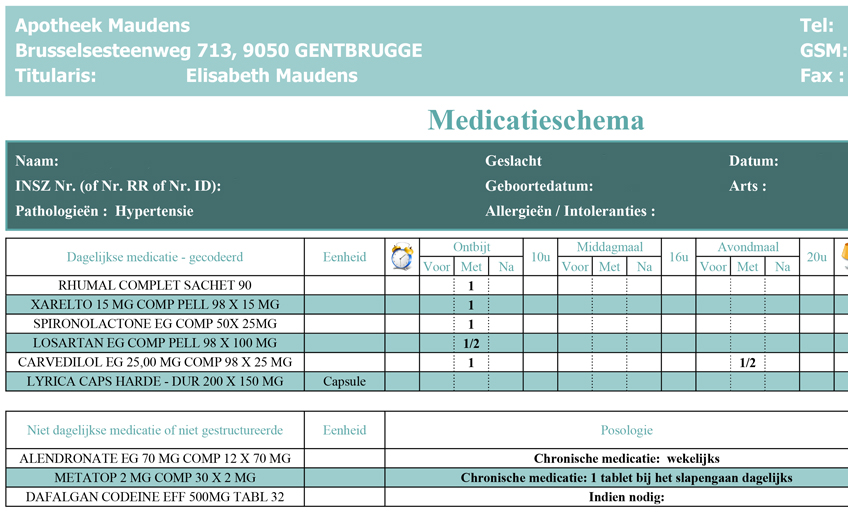
\includegraphics[width=1\textwidth]{img/voorbeeld_medicatieschema.jpg}
    \caption{Voorbeeld medicatieschema. Bron: apotheektsjoen.be}
    \label{fig:voorbeeld_medicatieschema}
\end{figure}

Zoals men in figuur \ref{fig:voorbeeld_medicatieschema} kan zien, wordt dit schema grafisch in tabulaire vorm gepresenteerd. Echter is de lay-out hiervan niet gestandaardiseerd; afhankelijk van de apotheker of andere zorgverstrekker worden andere kolomnamen, kolomverdeling, rand- en verdelingstijl, celgrootte en andere tabelelementen aangewend. Dit bemoeilijkt ernstig het ontwikkelen van een transformatiesysteem die ingescande medicatieschema’s omzet in instanties van een uniform digitale datastructuur in bv. XML- of JSON-formaat voor digitale verwerking van de medicatiedata in gezondheidszorgplatformen.

Een open source tabeltransformatiesoftware zal automatisch medicatieschema’s kunnen omzetten in een uniform digitale datastructuur. Hierdoor zal er geen manuele werk uitgevoerd moeten worden, wat tijd- en kostenreductie als positieve gevolgd heeft. Daarbovenop, omdat het open source zal zijn, zal men verzekerd zijn dat Into.care niet zal te maken hebben met softwarelicentiekosten of privacyschending.

% TODO: schema tabeltransformatiesoftware die medicatieschema omzet in JSON

Hoewel het digitaliseren van medicatieschema’s een belangrijke toepassing is, zijn er tal van andere potentiële toepassingen, aangezien tabellen zo vaak gebruikt worden. Zo zou men tabeltransformatie eveneens kunnen gebruiken voor het inscannen van kassatickets, het analyseren van een sudokuspel, het digitaal weergeven van een - op een whiteboard gemarkeerde - matrix voor online leerplatformen, het verwerken van een foto van een voedingswaardetabel op de verpakking van voedsel, en meer. Het is duidelijk dat een open source tabeltransformatiesoftware een beduidende universeel meerwaarde zal aanbieden.

% TODO: compilatie voorbeelden tabellen

\section{Onderzoeksvraag}
\label{sec:onderzoeksvraag}

Men kan zich bij tabeltransformatie, en dus bij dit onderzoek, enkele vragen stellen.

\begin{itemize}
    \item Uit welke processen bestaat tabeltransformatie? In welke volgorde deze plaats?
    \item Hoe kan men de performantie van tabeltransformatiesoftware best evalueren?
    \item Is preprocessing van de afbeelding nodig om de nauwkeurigheid van de resultaten te bewaren? Indien ja, uit welke stappen bestaat deze preprocessing?
    \item Analoog, is postprocessing van de verkregen tabel noodzakelijk? Indien ja, uit welke stappen bestaat deze postprocessing?
    \item Op welke manieren kan men de resultaten verbeteren, indien men in bezit is van domeinkennis? Zo zou men bijvoorbeeld kennis van de gezondheidszorg kunnnen gebruiken om medicatieschema’s nauwkeuriger te digtaliseren.
\end{itemize}

\section{Onderzoeksdoelstelling}
\label{sec:onderzoeksdoelstelling}

Aangezien het doel van deze studie het creëren van een end-to-end tabeltransformatie-tool is, zal er niet alleen gestreefd worden subprocessen zoals \Gls{OCR} of preprocessing geïsoleerd te bestuderen maar evenwel de subprocessen te implementeren in code. Eveneens is het de bedoeling dat de componenten met elkaar op een geïntegreerde manier zullen kunnen functioneren.

Dit betekent dat de prototype niet enkel zal bestaan uit tabelanalysesoftware, maar alsook uit een \Gls{GUI}, een backend server, een preprocessing pipeline, en meer. 

\section{Opzet van deze bachelorproef}
\label{sec:opzet-bachelorproef}

% Het is gebruikelijk aan het einde van de inleiding een overzicht te
% geven van de opbouw van de rest van de tekst. Deze sectie bevat al een aanzet
% die je kan aanvullen/aanpassen in functie van je eigen tekst.

De rest van deze bachelorproef is als volgt opgebouwd:

In Hoofdstuk~\ref{ch:stand-van-zaken} wordt een overzicht gegeven van de stand van zaken binnen het onderzoeksdomein, op basis van een literatuurstudie.

Verder wordt in Hoofdstuk~\ref{ch:methodologie} de methodologie toegelicht en worden de gebruikte onderzoekstechnieken besproken om een antwoord te kunnen formuleren op de onderzoeksvragen.

In Hoofdstuk~\ref{ch:proof-of-concept} wordt vervolgens de architectuur van de proof of concept uitgelegd. Eveneens worden de verschillende algoritmen in detail besproken.

Verder worden in Hoofdstuk~\ref{ch:resultaten} de met de proof of concept verkregen resultaten besproken en vergeleken.

In Hoofdstuk~\ref{ch:optimalisatiemogelijkheden} worden enkele optimalisatiemogelijkheden om de nauwkeurigheid van het systeem te verhoden, besproken.

En tenslotten in Hoofdstuk~\ref{ch:conclusie},  wordt de conclusie gegeven en een antwoord geformuleerd op de onderzoeksvragen. Daarbij wordt ook een aanzet gegeven voor toekomstig onderzoek binnen dit domein.



\chapter{Stand van zaken}
\label{ch:stand-van-zaken}

% Tip: Begin elk hoofdstuk met een paragraaf inleiding die beschrijft hoe
% dit hoofdstuk past binnen het geheel van de bachelorproef. Geef in het
% bijzonder aan wat de link is met het vorige en volgende hoofdstuk.

% Pas na deze inleidende paragraaf komt de eerste sectiehoofding.

In dit hoofdstuk wordt de stand van zaken besproken wat tabeltransformatie van afbeeldingen betreft. Er wordt besproken wat tabulair data is, waarom tabellen belangrijk zijn in de huidige informatiewereld, wat er bedoeld wordt met tabeldetectie en structuuranalyse, waar de uitdagingen hierbij zich bevinden en tenslotte wordt er in detail de verschillende technieken besproken die ontwikkeld werden om tabellen te kunnen detecteren en analyseren, met hun voor- en nadelen.

\section{Tabulair data}
\label{sec:tabulair-data}

\subsection{Definitie}
\label{subsec:definitie-tabulair-data}

Zoals \textcite{Zanibbi2003} het aangeeft, is een tabel een vorm van visualiatie dat men gebruikt om ermee data op te zoeken en te vergelijken. Meer specifiek geeft, volgens \textcite{Zanibbi2003}, een tabel indexeringschema's weer voor relaties. Een relatie heeft een verzameling van $\eta$ \glspl{tupel}, die de domeinen of dimensies van de relatie genoemd worden.

De dimensies kunnen d.m.v. verschillende combinaties van rijen en kolommen opgesteld worden, waardoor verschillende tabelopstellingen exact dezelfde informatie op verschillenden manieren kunnne weergeven. Dit kan gedemonstreerd worden a.d.h.v. de volgende twee figuren.

\begin{figure}[H]
    \centering
    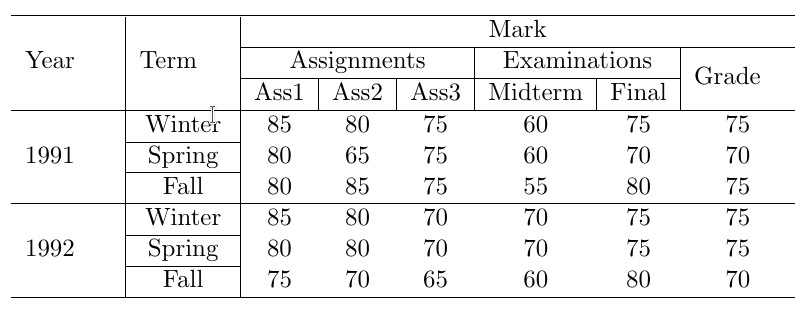
\includegraphics[width=0.8\textwidth]{img/tabel_verschillende_opstelling_dezelfde_data_1.png}
    \caption{Een tabel van evaluaties. Het geeft dezelfde informatie weer als tabelfiguur \ref{fig:tabel_verschillende_opstelling_dezelfde_data_2}. Bron: \cite{Long2010}}
    \label{fig:tabel_verschillende_opstelling_dezelfde_data_1}
\end{figure}

\begin{figure}[H]
    \centering
    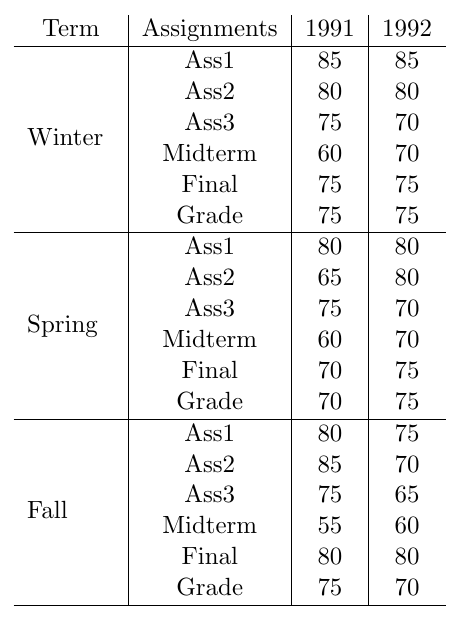
\includegraphics[width=0.5\textwidth]{img/tabel_verschillende_opstelling_dezelfde_data_2.png}
    \caption{Een tabel van evaluaties. Het geeft dezelfde informatie weer als tabelfiguur \ref{fig:tabel_verschillende_opstelling_dezelfde_data_1}. Bron: \cite{Long2010}}
    \label{fig:tabel_verschillende_opstelling_dezelfde_data_2}
\end{figure}

Hoewel beide tabellen identiek zijn wat informatieinhoud betreft, kan duidelijk gemerkt worden dat tabelfiguur \ref{fig:tabel_verschillende_opstelling_dezelfde_data_1} de evaluaties duidelijker weergeeft. Meestal wordt een combinatie van rijen en kolommen zodanig gekozen zodat de data van de tabel zo eenvoudig en snel mogelijk gelezen en geïnterpreteerd kan worden. Ook kunnen verschillende lettertypes, kleuren en lettergroottes gebruikt worden om de leesbaarheid te vergroten.

\subsection{Anatomie}
\label{subsec:anatomie}

\raggedbottom

Volgens \textcite{Wang1996} is een tabel, door \textit{stub scheiding} en \textit{boxhead scheiding}, verdeeld in vier hoofdregio's die in onderstaande figuur \ref{fig:tabel_anatomie} merkbaar zijn. De regio linksbeneden die de rijhoofdingen bevat en de regio rechtsboven die de kolomhoofdingen bevat, worden respectievelijk de \textit{stub} en de \textit{boxhead} genoemd. De regio linksboven, die de categorieën in de \textit{stub} inhouden is gekend als de \textit{stub head} en de \textit{body} tenslotte, is de regio rechts van de \textit{sub} en onder de \textit{boxhead} die de tabeldata-elementen bevat. De snijpunt van een rij en een kolom wordt een \textit{cel} genoemd; en een rechthoekig verzameling van \textit{cellen} is gekend als een \textit{block}.

\begin{figure}[H]
    \centering
    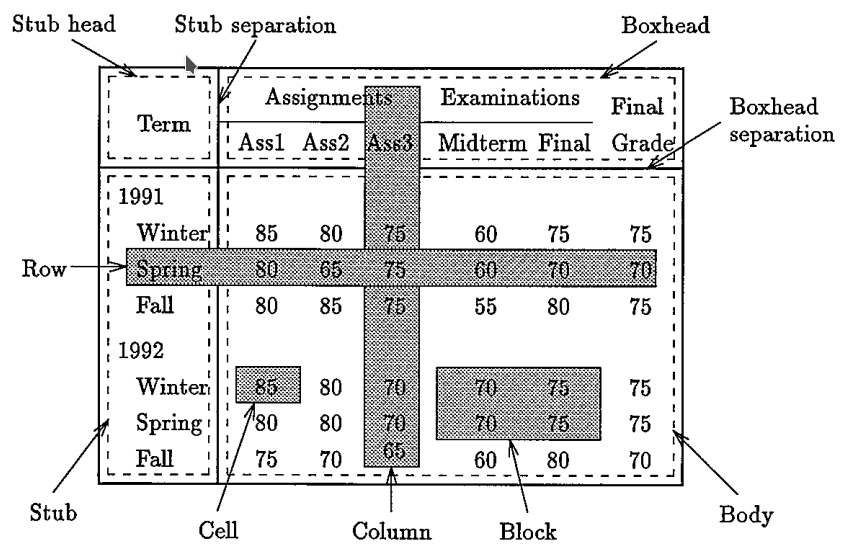
\includegraphics[width=0.8\textwidth]{img/tabel_anatomie.png}
    \caption{De anatomie van de structurele rij-kolomvoorstelling van een tabel. Bron: \cite{Wang1996}}
    \label{fig:tabel_anatomie}
\end{figure}

Zoals men in figuur \ref{fig:tabel_anatomie} kan zien, kunnen multidimensionele relaties in een twee dimensionele tabel gepresenteerd worden door meer dan één categorie te associeren met de \textit{boxhead} en/of met de \textit{stub}. Zo worden hier de rijhoofdingen niet enkel met één hoofdcategorie ``Term`` maar eveneens met meerdere subcategorieën, ``1991`` en ``1992`` geassocieerd. Analoog zijn de kolomhoofdingen gekoppeld aan drie categorieën, namelijk ``Assignments``, ``Examinations`` en ``Finals``.

\subsection{Functie}
\label{subsec:functie}

Als vermeld door \textcite{Shahzad2019}, worden tabellen veelal gebruikt voor het gestructureerd vertonen van essentiële informatie in documenten. Ze worden gebruikt in boeken, artikelen, onderzoekspapers, en verschillende andere soorten media. In sectoren zoals de financiële en de administratieve sectoren wordt data veelal in tabelvorm geformuleerd omdat tabellen, volgens \textcite{Coueasnon2014}, veel informatie voorstellen op een beknopte manier waardoor het begrijpbaar blijft voor de lezer; ze laten ook zo toe de belangrijke delen te benadrukken. 

\subsection{Creatie en representatie}
\label{subsec:creatie-en-representatie}

Doorheen de tijd werden verschillende software applicaties ontwikkeld om digitaal tabulair data aan te maken, te beheren en voor te stellen. Een veelgebruikte software voor tabelcompositie is Microsoft Excel. Het is, zoals \textcite{Wang1996} het vermeldt, een complexe rekenbladprogramma waarbij tabulair data in een werkblad, in een twee dimensionele rooster die a.d.h.v. rij en kolomindexes geadresseerd kan worden, geplaatst wordt.

Een andere bekend software voor het creëren van tabellen is \LaTeX. Het is een systeem voor het zetten van documenten. \textcite{Wang1996} geeft aan dat tabellen in \LaTeX\ gespecifieerd kunnen worden met de ``tabular``- en de ``array``-omgeving. De eerste omgeving wordt meestal gebruikt voor tekstuele tabeldata, de tweede voor wiskundige uitdrukkingen.

Voor de voorstelling van tabellen op het internet, m.a.w. op internetbrowsers, wordt de opmaaktaal HTML gebruikt. Door middel van de ``table``-, ``tr``-, ``th``- en ``td``-tags kunnen tabellen gemaakt en voorgesteld worden.

\section{Tabeltransformatie}
\label{sec:tabel-transformatie}

Verschillende technieken om tabeltransformatie werden reeds ontwikkeld. Echter blijft een algemeen toepasbare oplossing een moeilijk uitdaging, en dit voor diverse redenen.

\begin{itemize}
    \item Tabellen bezitten uiteenlopende layouts en designs, zonder enige standaardisatie
          \autocite{Kasar2014}
    \item Verschillende tabellayouts hebben verschillende features \autocite{Kasar2014}
    \item De typisch kleine inter-klasse variantie tussen tabellen, figuren en grafieken vermoeilijkt
          de detectie van tabellen; de kleine variantie is verantwoordelijk voor de hoge hoeveelheid
          valse positieven bij tabeldetectie \autocite{Embley2006}
  \end{itemize}

\textcite{Kasar2014} beschreeft tabeltransformatie als een proces bestaand uit voornamelijk twee subprocessen: tabeldetectie en tabelstructuuranalyse. 

Met tabeldetectie worden eerst regio's in een bepaalde document geïdentificeerd die overeenkomen met tabellen. Vervolgens wordt tabelstructuuranalyse toegepast om relationele informatie te extraheren van de geïdentificeerde tabelregio's om de logische structuur van de tabellen te achterhalen, zoals bijvoorbeeld de rijhoofdingen, kolommhoofdingen, cellen en meer.

\subsection{Tabeldetectie}
\label{subsec:tabel-detectie}

Tabeldetectietechnieken kan men, kijkend naar de stand van zaken, opdelen in twee klassen: klassieke, op regelgebaseerde algoritmen enerzijds en de recentere, opkomende algoritmen die gebruik maken van machinaal leertechnieken.

\subsubsection{Regelgebaseerde technieken}

\textcite{Watanabe1991} was de auteur van één van de vroegste werken om tabellen te identificeren. De basis voor de tabelidentificatie hier is de identificatie van individuele blokken, ingesloten door horizontale en verticale lijnsegmenten. Eerst worden lijnsegmenten gedetecteerd en hiermee wordt vervolgens de positie van hoekpunten, gevormd door deze lijne, bepaald. Hierna wordt a.d.h.v. de poositie van deze hoekpunten individuele blokken geïdentificeerd. De relatie tussen de verschillende blokken wordt uiteindelijk in globale en individuele boomstructuren gebruikt om te beslissen of het over een tabel gaat of niet.

Het jaar daarop stelde \textcite{Laurentini1992} een methode voor waarbij tekstregio's op een bottom-up manier gedetecteerd worden. De gedetecteerde karakters worden samengebracht tot woorden en deze woorden worden op hun beurt aan elkaar samengevoegd tot tekstblokken. Ook worden de scheidingslijnen gedeteceerd. Voor elke tekstblok wordt diens positie vergeleken met de scheidingslijnen, om te bepalen of het tot een bepaalde tabel behoort.

TINTIN werd door \textcite{Pyreddy1997} voorgesteld, om tabellen te detecteren. Hun algoritme steunt voor de analyse op de extra PDF-metadata van de PDF-documenten.

Enkele jaren later werd het systeem T-Recs, door \textcite{Kieninger2001}, voorgesteld. Het systeem vormt rechthoeken (bounding boxes) voor woorden in het tabel en op een bottom-up manier worden deze bounding boxes gegroepeerd volgens hun logische eenheden. 

\subsubsection{Datagedreven technieken}

\subsection{Tabelstructuuranalyse}
\label{subsec:tabel-structuur-analyse}

\subsection{End-to-end-systemen}
\label{subssec:end-to-end-systemen}

%%=============================================================================
%% Methodologie
%%=============================================================================

\chapter{Methodologie}
\label{ch:methodologie}

%% TODO: Hoe ben je te werk gegaan? Verdeel je onderzoek in grote fasen, en
%% licht in elke fase toe welke stappen je gevolgd hebt. Verantwoord waarom je
%% op deze manier te werk gegaan bent. Je moet kunnen aantonen dat je de best
%% mogelijke manier toegepast hebt om een antwoord te vinden op de
%% onderzoeksvraag.

In dit hoofdstuk worden eerst het doel en de systeemvereisten van de proof-of-concept besproken. Vervolgens wordt de selectie van technologieën voor de proof-of-concept behandeld, inclusief de keuze van de tabelstransformatie-algoritme(n). Uiteindelijk wordt de evaluatiessyteem verduidelijkt die gebruikt wordt om de performantie van de proof-of-concept te beoordelen.

\section{Systeemvereisten}
\label{sec:systeemvereisten}

\subsection{Goals}

Om een proof-of-concept succesvol te kunnen realiseren, moeten de volgende einddoelen hiervoor bereikt worden:

\begin{itemize}
    \item Een end-to-end-systeem dient gecreëerd te worden. Dit betekent dat de proof-of-concept niet enkel een tabeldetectiecomponent moet bevatten, maar eveneens een tabelstructuuranalysecomponent, een GUI en andere nodige elementen om de tabeltransformatie zoveel mogelijk te automatiseren.\\

    \item De software moet modulair geïmplementeerd worden. Code geschreven voor tabeldetectie, bijvoorbeeld, mag niet afhankelijk zijn van code geschreven voor tabelstructuuranalyse en vice versa. Dit maakt het mogelijk om later één deel van de tabeltransformatiesoftware te verbeteren of opnieuw te herschrijven, zonder hierdoor een impact te hebben op de rest van de software.\\

    \item Enkel open source software en libraries, zonder commercële restricties, mogen gebruikt worden.\\

    \item De proof-of-concept moet kunnen functioneren op verschillende eenvoudige tabellayouts. D.w.z. dat de tabeltransformatie niet mag afhangen van de fysieke dimensies van de tabel zelf of van de cellen. Noch mag het afhankelijk zijn van het aantal rijen of kolommen. Verder moet de software contextonafhankelijk zijn; een voedingswaardetabel bijvoorbeeld moet even nauwkeurig getransformeerd kunnen worden als een medicatieschema.\\

    \item Een tabeltransformatie moet kunnen uitgevoerd worden door een \Gls{REST}-server op te roepen. De tabeltransformatieresultaat die de server bij deze terug zal geven, moet een intuïtief, goed opgesteld \Gls{JSON}-object zijn.
\end{itemize}

\subsection{Non-goals}

Naast einddoelen die de scope van de proof-of-concept vormen zijn er eveneens non-goals, vereisten die expliciet buiten de scope liggen:

\begin{itemize}
    \item Het is niet de bedoeling om een volledige softwarepakket te ontwikkelen, met error handling, unit tests, integratie tests, authenticatie en meer.\\

    \item De proof-of-concept moet niet complexe tabellen kunnen verwerken. Hiermee worden voornamelijk tabellen bedoelt met meerdere niveau's van rijen en kolommen of tabellen met subtabellen.\\

    \item Preprocessing van de inputafbeeldingen wordt niet uitgevoerd. Er wordt verwacht dat de documenten correct zijn ingescand.\\

    \item Tabellen met handgeschreven tekst worden niet in beschouwing genomen.
\end{itemize}

\section{Selectie technologieën}
\label{sec:selectie-technologieën}

Op basis van de literatuurstudie (\autoref{ch:stand-van-zaken}) en de systeemvereisten (\autoref{sec:systeemvereisten}) kan de selectie van algoritmes en technologieën plaatsvinden.

\subsection{Tabeldetectie en Tabelstructuuranalyse}

De verschillende algoritmes voor tabeldetectie en tabelstructuuranalyse, behandeld in de literatuurstudie (\autoref{ch:stand-van-zaken}), hebben elk hun voor- en nadelen. Deze voor- en nadelen worden in de volgende tabel \ref{tab:voor-en-nadelen-tabel-transformatie-technieken} weergegeven.

\begin{table}[H]
\centering
\begin{tabular}{@{}lccc@{}}
\toprule
                            & Werkt zonder lijnen & Bruikbaar op afbeelding & Diverse layouts \\ \bottomrule
\multicolumn{4}{c}{\textit{Tabeldetectie}}                                                    \\ \toprule
\citeauthor{Watanabe1991}   &                     & \checkmark              & \checkmark      \\ \midrule
\citeauthor{Laurentini1992} &                     & \checkmark              & \checkmark      \\ \midrule
\citeauthor{Pyreddy1997}    & \checkmark          &                         & \checkmark      \\ \midrule
\citeauthor{Kieninger2001}  & \checkmark          & \checkmark              &                 \\ \midrule
\citeauthor{Cesarini2002}   &                     & \checkmark              & \checkmark      \\ \midrule
\citeauthor{Mandal2006}     & \checkmark          & \checkmark              &                 \\ \midrule
\citeauthor{Silva2009}      &                     &                         & \checkmark      \\ \midrule
\citeauthor{Kasar2013}      &                     & \checkmark              & \checkmark      \\ \midrule
\citeauthor{Fan2015}        & \checkmark          & \checkmark              & \checkmark      \\ \midrule
\citeauthor{Tran2015}       & \checkmark          & \checkmark              & \checkmark      \\ \midrule
\citeauthor{Hao2016}        &                     &                         &                 \\ \midrule
\citeauthor{Rashid2017}     & \checkmark          & \checkmark              &                 \\ \midrule
\citeauthor{Gilani2017}     & \checkmark          & \checkmark              & \checkmark      \\ \midrule
\citeauthor{Siddiqui2018}   & \checkmark          & \checkmark              & \checkmark      \\ \bottomrule
\multicolumn{4}{c}{\textit{Tabelstructuuranalyse}}                                            \\ \toprule
\citeauthor{Nazemi2016}     &                     & \checkmark              & \checkmark      \\ \midrule
\citeauthor{Qasim2019}      & \checkmark          & \checkmark              & \checkmark      \\ \bottomrule
\multicolumn{4}{c}{\textit{End-to-end-systemen}}                                              \\ \toprule
\citeauthor{Green1996}      &                     & \checkmark              &                 \\ \midrule
\citeauthor{Oro2009}        & \checkmark          &                         & \checkmark      \\ \midrule
\citeauthor{Schreiber2017}  & \checkmark          & \checkmark              & \checkmark      \\ \midrule
\citeauthor{Prasad2020}     & \checkmark          & \checkmark              & \checkmark      \\ \bottomrule
\end{tabular}
\caption{Voor- en nadelen van tabeltransformatiealgoritmes}
\label{tab:voor-en-nadelen-tabel-transformatie-technieken}
\end{table}

Wat tabeldetectie betreft, bieden de algoritmes \autocite{Tran2015}, \autocite{Gilani2017} en \autocite{Siddiqui2018} alle voordelen aan. Alle drie technieken werken zonder de aanwezigheid van horizontale of verticale tabelscheidingslijnen. Ze kunnen direct gebruikt worden op afbeeldingen, en zijn dus niet afhankelijk van PDF-metadata bijvoorbeeld. Tenslotte kunnen ze tabellen van verschillende layouts detecteren.

Van de technieken voor tabelstructuuranalyse heeft \autocite{Qasim2019} alle voordelen.

Tenslotte bieden de end-to-end-technieken, \autocite{Schreiber2017} en \autocite{Prasad2020}, eveneens alle voordelen.

Om het aantal kandidaatalgoritmes voor de proot-of-concept verder te verminderen, worden hun performanties met elkaar vergeleken. Omdat voor de tabelstructuuranalyse geen algoritmes te vinden zijn wiens performantiemeting met dezeflde methodologie uitgevoerd is, worden deze performanties niet in rekening gehouden. In onderstaande tabel \ref{tab:tabel-detectie-performanties} kan men de performantie van de verschillende technieken voor tabeldetectie terugvinden.

\begin{table}[H]
\centering
\begin{tabular}{@{}lccc@{}}
\toprule
                           & \Gls{Recall} & \Gls{Precisie} & \Gls{F1-score} \\ \midrule
\citeauthor{Tran2015}      & 0,9636       & 0,9521         & 0,9578         \\ \midrule
\citeauthor{Gilani2017}    & 0,9067       & 0,8230         & 0,8629         \\ \midrule
\citeauthor{Siddiqui2018}  & 0,996        & 0,996          & 0,996          \\ \midrule
\citeauthor{Schreiber2017} & 0,9615       & 0,9740         & 0,9677         \\ \midrule
\citeauthor{Prasad2020}    & 1,0          & 1,0            & 1,0            \\ \bottomrule
\end{tabular}
\caption{Tabeldetectieperformanties van de verschillende algoritmes}
\label{tab:tabel-detectie-performanties}
\end{table}

Deze performantiemetingen werden uitgevoerd op de \citefield{Gobel2013}{title} dataset. Dit is één van de meest bekende datasets voor tabeldetectie en tabelstructuuranalyse. Het bevat in totaal 238 ingescande documenten. Voor de berekening van de \Gls{F1-score} wordt bij deze dataset een \Gls{IoU} threshold van 0,5 gebruikt.

Aangezien de tabeldetectiealgoritme van \textcite{Prasad2020} de meest performante is, wordt deze geselectioneerd als de tabeldetectiecomponent van de proof-of-concept. Voor de tabelstructuuranalyse kan men nog kiezen tussen \autocite{Qasim2019}, \autocite{Schreiber2017} en opnieuw \autocite{Prasad2020}. Hoewel \autocite{Qasim2019} en \autocite{Schreiber2017} gepaste keuzes zijn, wordt er beslist om voor de structuuranalyse eveneens \autocite{Prasad2020} te selectioneren. Dit komt voornamelijk omdat \textcite{Prasad2020} niet enkel hun volledige modeltrainingdataset maar ook de code-implementatie van hun algoritme openbaar hebben gemaakt, met een open source licentie.

\subsection{Programmeertaal}

Voor de programmeertaal van de proof-of-concept wordt Python \autocite{VanRossum2009} gekozen, en dit voor verschillende redenen:

\begin{itemize}
    \item Python is een multifunctioneel programmeertaal die toelaat om eenvoudig en snel softwareprototypes te creëren.\\

    \item Het heeft een grote bibliotheek van libaries voor onder meer statistiek en data-analyse, zoals Numpy \autocite{Oliphant2006} en Pandas \autocite{McKinney2010}.\\

    \item De open source code van \textcite{Prasad2020} is reeds in Python geschreven. Door met Python verder te werken, kan code herbruikt worden en zal een een volledig nieuwe reïmplementatie van de software dus niet nodig worden.
\end{itemize}

\subsection{Interne tabelmodel}

Om de getransformeerd tabel te kunnen verwerken en verbeteren, moet de software van de proof-of-concept deze d.m.v. een datastructuur bijhouden. Hoewel voor de datastructuur JSON of XML gekozen kan worden, wordt er beslist om intern de getransformeerd tabel te presenteren en te verwerken d.m.v. een Pandas Dataframe. Een Pandas Dataframe is een twee dimensionele tabulaire datastructuur van de Pandas library. Deze datastructuur bestaat voornamelijk uit drie hoofdcomponenten, die in onderstaande figuur worden weergegeven: rijen, kolommen en data.

\begin{figure}[H]
    \centering
    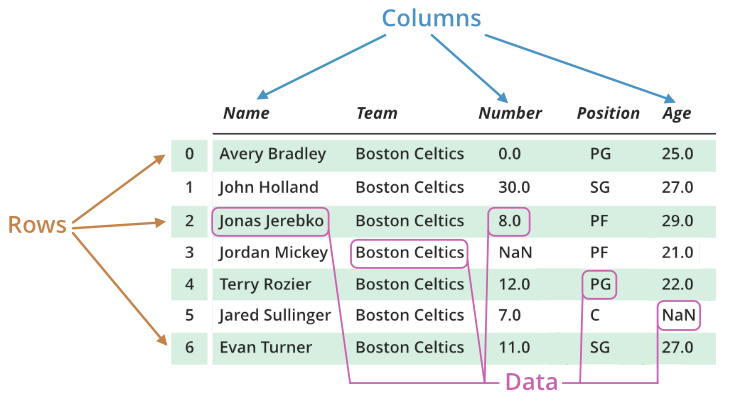
\includegraphics[width=0.8\textwidth]{img/pandas_dataframe.png}
    \caption{Anatomie van een Pandas Dataframe. Bron: \textcite{GeeksforGeeks2020}}
    \label{fig:anatomie-pandas-dataframe}
\end{figure}

Niet enkel modelleert een Pandas Dataframe, met zijn twee dimensionele structuur, op een gepaste manier een tabel maar het bezit eveneens andere voordelen. Zo kan de opgeslagen data heterogeen zijn, d.w.z. dat de datatypes van de data-elementen niet identiek hoeven te zijn. Verder bezit het meerdere functionaliteiten om data eenvoudig te manipuleren. Tenslotte kan een Pandas dataframe zeer efficiënt met grote hoeveelheden data werken.

\subsection{\Gls{OCR}}

Voor de \Gls{OCR}-component zijn er niet veel keuzes. Tesseract \autocite{Kay2007} is momenteel de enige \Gls{OCR}-software die open source is en nauwkeurig tekst in afbeeldingen detecteert en transformeert. Bovendien kan de Python library, Pytesseract \autocite{Lee2009}, gebruikt worden om Tesseract-functionaliteiten met Python te gebruiken. Zo kan men Tesseract functionaliteiten d.m.v. Pytesseract in Python code oproepen en kunnen de \Gls{OCR}-resultaten als een Pandas Dataframe verkregen worden.

\subsection{Back end server}

Voor de \Gls{REST}-server wordt Flask \autocite{Grinberg2018} gekozen. Flask is een eenvoudige micro web framework, bedoeld voor Python-softwareontwikkeling, met \Gls{REST}-ondersteuning.

\subsection{Front end}

Er bestaan verschillende front end frameworks om snel en eenvoudig GUI's te ontwerpen die via de browser gebruikt zullen kunnen worden, zoals Angular \autocite{Jain2014} en React \autocite{Fedosejev2016}. Voor deze proof-of-concept wordt React gebruikt, in combinatie met de UI framework Ant Design \autocite{Financial2020}. De UI framework Ant Design biedt herbruikbare UI-componenten, onder meer voor tabulair data, die de ontwikkeling van de proof-of-concept vereenvoudigen en versnellen.

%%=============================================================================
%% Proof of concept
%%=============================================================================

\chapter{Proof of concept}
\label{ch:proof-of-concept}

De proof-of-concept wordt in dit hoofdstuk in detail behandeld. De verantwoordelijkheid en werking van de verschilende componenten wordt uitgelegd. Hiernaast wordt de flow (stroom) van de data verduidelijkt. Tenslotte wordt de installatie van de proof-of-concept-software uitgelegd.

\section{Architectuur}
\label{sec:architectuur}

\begin{figure}[H]
    \centering
    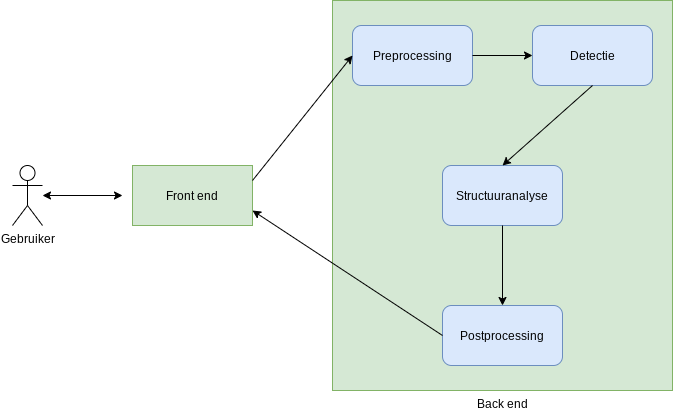
\includegraphics[width=1\textwidth]{img/proof_of_concept_architectuur.png}
    \caption{Architectuur van de proof-of-concept.}
    \label{fig:architectuur-proof-of-concept}
\end{figure}

In figuur \ref{fig:architectuur-proof-of-concept} wordt de architectuur van de proof-of-concept weergegeven, inclusief de verschillende componenten zoals \Gls{OCR}, tabeldetectie en meer. De datastroom, samen met de werking van de componenten, wordt in de volgende subsecties verder toegelicht.

\subsection{Documentinput}
\label{subsec:document-input}

Wanneer de gebruiker de software wil gebruiken, zal hij/zij een GUI zien die in de volgende figuur weergegeven wordt.

\begin{figure}[H]
    \centering
    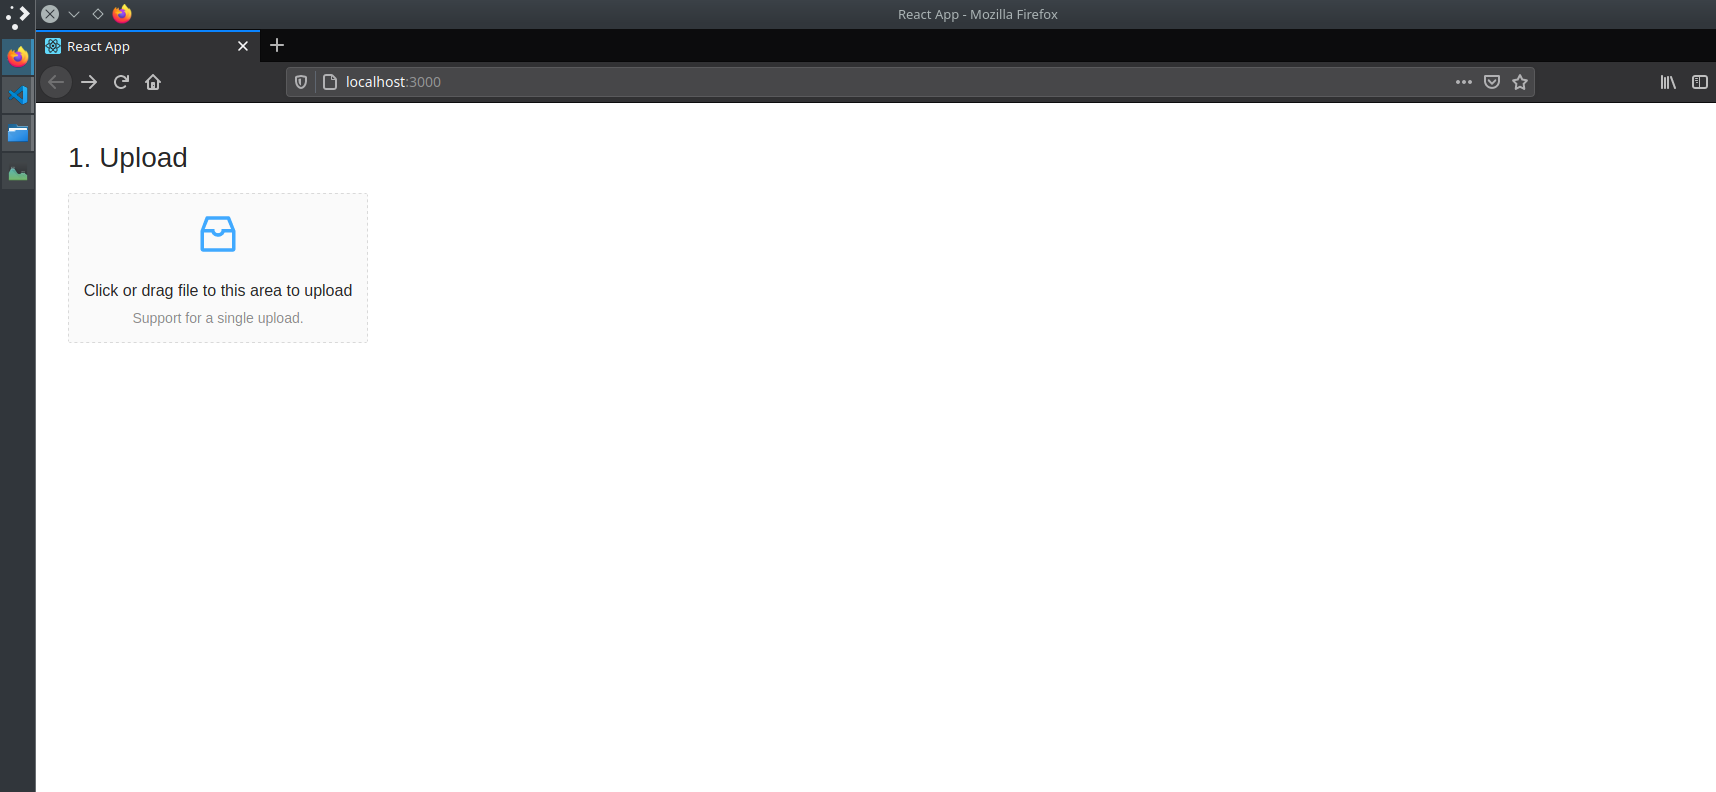
\includegraphics[width=1\textwidth]{img/gui_screenshot_not_used.png}
    \caption{GUI van de software bij eerste gebruik.}
    \label{fig:gui-screenshot-not-used}
\end{figure}

De gebruiker klikt op de upload-zone, waar de tekst ``Click or drag file to this area to upload`` vermeld staat. Vervolgens selecteert de gebruiker de document die getransformeerd moet worden. Bij de bevestiging van de selectie van het bestand wordt deze geüpload naar de back end, waar preprocessing plaatsvindt.

\subsection{Preprocessing}
\label{subsec:preprocessing}

Bij de preprocessing wordt extra witruimte toegevoegd aan de afbeelding. Dit is nodig omdat de tabeldetectiealgoritme, hoewel het zeer goed werkt op afbeeldingen van ingescande documenten, moeilijkheden heeft met tabeldetectie wanneer de afbeelding enkel uit de tabel zelf bestaat, zonder extra tekstelementen, witruimte, grafieken, figuren of dergelijke. Dit komt omdat de deep learning model getrained werd op documentafbeeldingen en niet op tabelafbeeldingen zelf. Eens de preprocessing uitgevoerd is, wordt tabeldetectie op de nieuwe afbeelding, waar extra witruimte aanwezig is, uitgevoerd.

\subsection{Tabeldetectie}
\label{subsec:tabel-detectie}

Voor de detectie wordt een drempel waarde (threshold) van 0,85 gekozen. Dit heeft als gevolg dat indien de berekende kans op de aanwezigheid van een tabel door de deep learning model gelijk is aan, of groter is dan 0,85, dan wordt de aanwezigheid van één of meerdere tabellen in de afbeelding als waar beschouwd; anders niet.

In onderstaande figuren \ref{fig:tabel-detectie-origineel} en \ref{fig:tabel-detectie-gedetecteerd} kan men respectievelijk links een origineel ingescande document zien en rechts de gedetecteerde tabellen in het document.

\begin{figure}[H]
    \centering
    \begin{minipage}{0.5\textwidth}
        \centering
        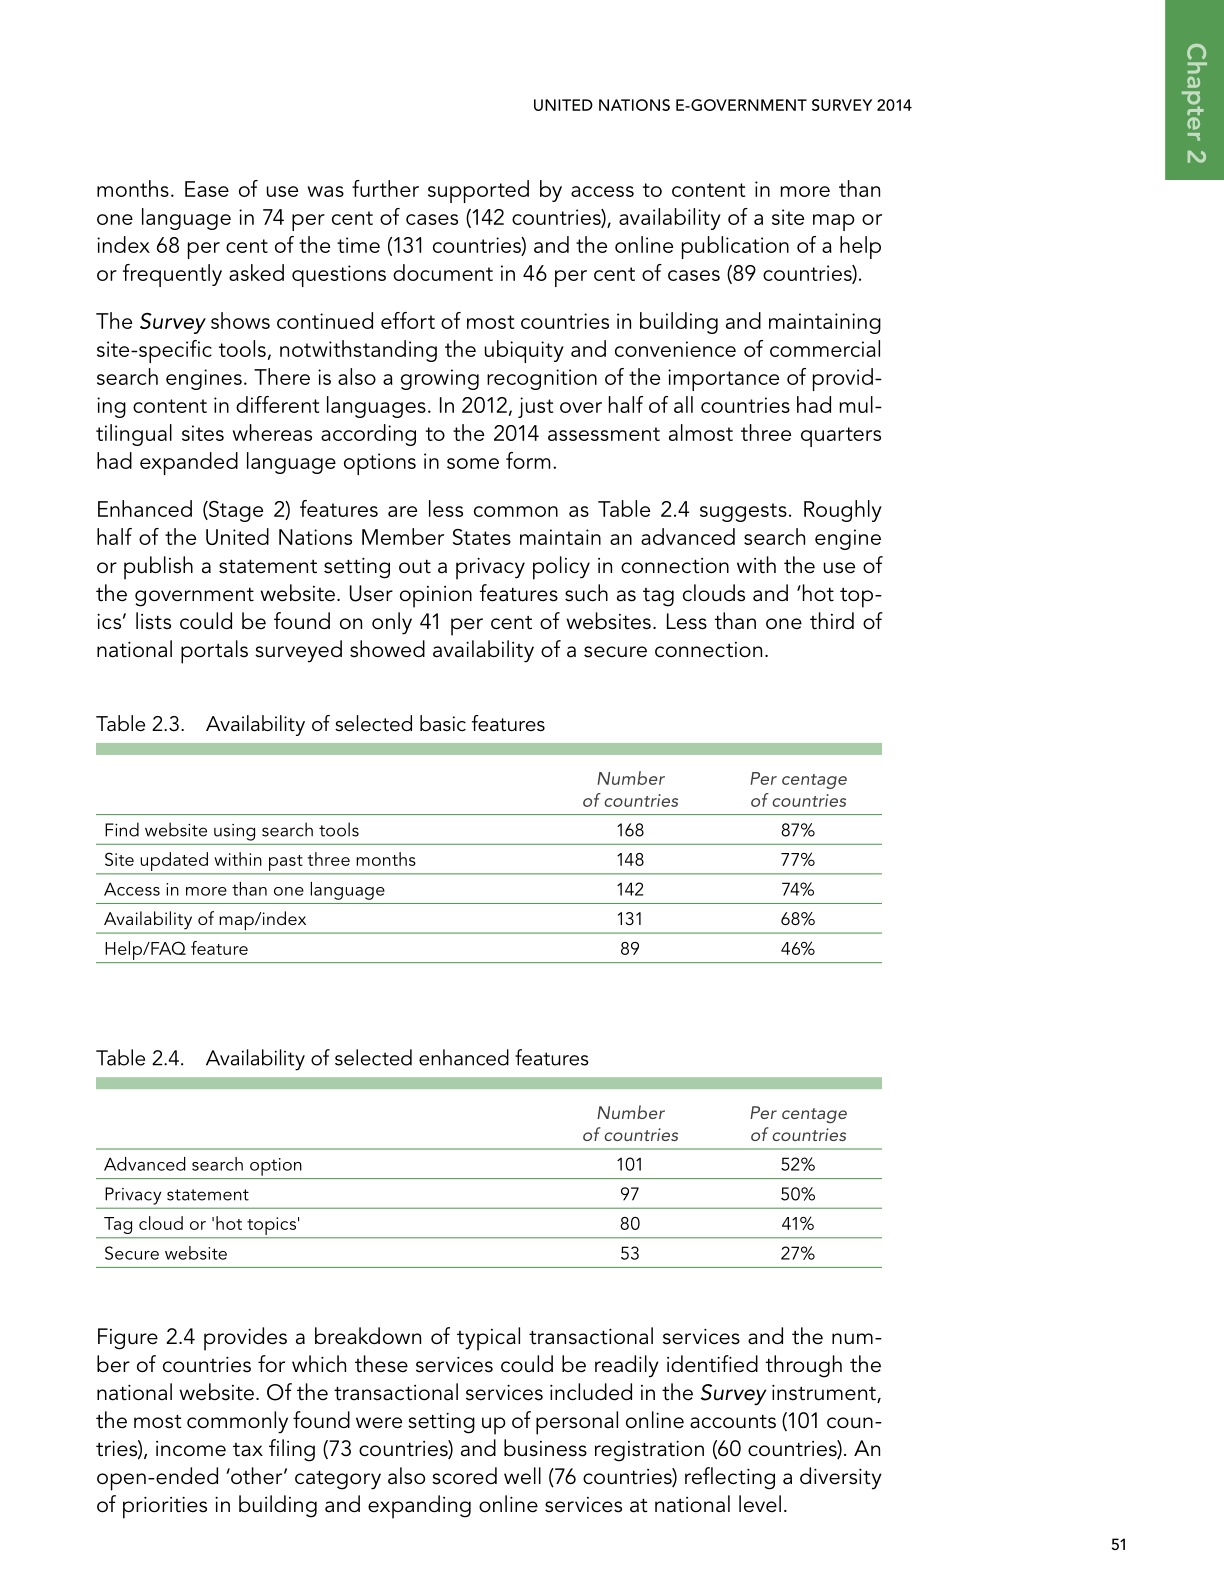
\includegraphics[width=1\textwidth]{img/tabel_detectie_voorbeeld_origineel.jpg}
        \caption{Origineel document}
        \label{fig:tabel-detectie-origineel}
    \end{minipage}\hfill
    \begin{minipage}{0.5\textwidth}
        \centering
        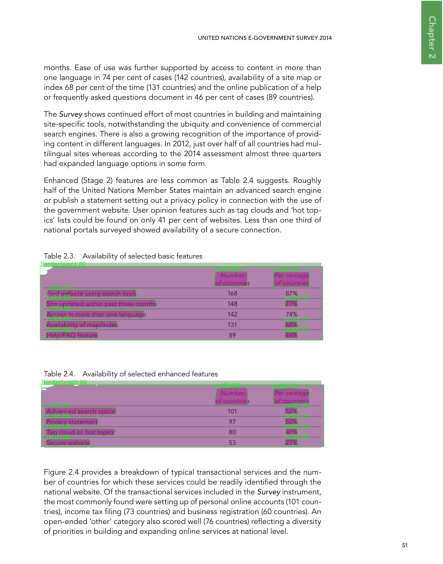
\includegraphics[width=1\textwidth]{img/tabel_detectie_voorbeeld_gedetecteerd.png}
        \caption{Gedetecteerde tabellen.}
        \label{fig:tabel-detectie-gedetecteerd}
    \end{minipage}
\end{figure}

Zoals men kan zien in figuur \ref{fig:tabel-detectie-gedetecteerd}, worden niet enkel de tabellen zelf maar eveneens cellen gedetecteerd. De detectie van tabellen is zeer accuraat, hoewel de detectie van cellen niet even nauwkeurig is. In de figuur bijvoorbeeld werden sommige cellen niet gedetecteerd.

Nadat de tabellen gedetecteerd zijn, worden ze bijgesneden om enkel de tabellen zelf te behouden en niet meer de rest van de document. Op elke geïsoleerd tabel worden de volgende stappen, tabelstructuuranalyse (\ref{subsec:tabel-structuur-analyse}) en postprocessing (\ref{subsec:post-processing}) uitgevoerd.

\subsection{Tabelstructuuranalyse}
\label{subsec:tabel-structuur-analyse}

\subsubsection{Origineel algoritme}
\label{subsubsec:origineel-algoritme}

Bij de tabelstructuuranalyse-algoritme van \textcite{Prasad2020}, die vanaf dit punt als ``algoritme A`` genoemd zal worden, wordt eerst gekeken naar de soort gedetecteerd tabel die bepaald en meegegeven werd door de tabeldetectie-component. Indien het om een bordered tabel gaat, wordt lijndetectie toegepast en wordt vervolgens d.m.v. cellsegmentatie aan elke cel een rij- en kolomwaarde toegekend. Anders, indien het dus als een borderless tabel gedetecteerd werd, wordt de positie van mogelijks gemiste, niet-gedetecteerde cellen voorspeld. De voorspelde cellen, samen met de reeds gedetecteerde cellen, worden vervolgens gebruikt om de rijen en kolommen te vormen.

Eens de tabel getransformeerd is, wordt het resultaat opgeslagen in een XML-bestand. Een voorbeeld hiervan wordt in de volgende code \ref{lst:xml-resultaat} weergegeven.\newpage

\lstinputlisting[language=XML, caption={Voorbeeld van een XML-resultaat-bestand.}, captionpos=b, label={lst:xml-resultaat}]{code/resultaat_tabelstructuuranalyse_voorbeeld.xml}

Daaropvolgend wordt de XML-resultaat-bestand geïtereerd. Bij een ``cell``-XML-tag wordt gekeken naar de coördinaten en dimensies (gespecifieerd door de ``Coords``-XML-tag van de ``cell``-tag) en op basis hiervan wordt \Gls{OCR} op enkel die regio toegepast. Hierdoor verkrijgt men de tekst te vinden binnen de celregio, gedefinieerd door de XML-resultaat. Dit proces wordt iteratief uitgevoerd op elke ``cell``-tag. Door middel van de tekst en rij- en kolomwaarden (gespecifieerd door respectievelijk de ``start/end-row``- en ``start/end-col``-attribuut) van elke cel wordt tenslotte een Pandas Dataframe aangemaakt die de getransformeerd tabel bevat.

\subsubsection{Voorgesteld verbeterd algoritme}
\label{subsubsec:origineel-algoritme}

In tabelafbeeldingen waarin voldoende ruimte aanwezig is tussen de cellen (in geval van borderless tabellen) of in tabelafbeeldingen waarin de horizontale en verticale scheidingslijnen goed te onderscheiden zijn van de rest van de tabel (in geval van bordered tabellen), is algoritme A bruikbaar. Echter, zoals reeds aangegeven, worden de cellen door de tabeldetectiemodel niet altijd gedetecteerd. Ook zijn tabelscheidingslijnen soms moeilijk te onderscheiden van andere lijnen, zoals de lijnen die gevormd worden door letters zoals de `l` of `p`. Door deze complicaties werkt algoritme A meestal niet.

Daarom worden enkele aanpassingen voorgesteld voor de tabelstructuuranalyse, die gezamenlijk als ``algoritme B`` genoemd zullen worden.

Voor bordered tabellen wordt een verbetering van de lijndetectie-algoritme voorgesteld.

De verschilende stappen die genomen worden bij lijndetectie worden gedemonstreerd d.m.v. de volgende figuur \ref{fig:lijn-detectie-origineel}.

\begin{figure}[H]
    \centering
    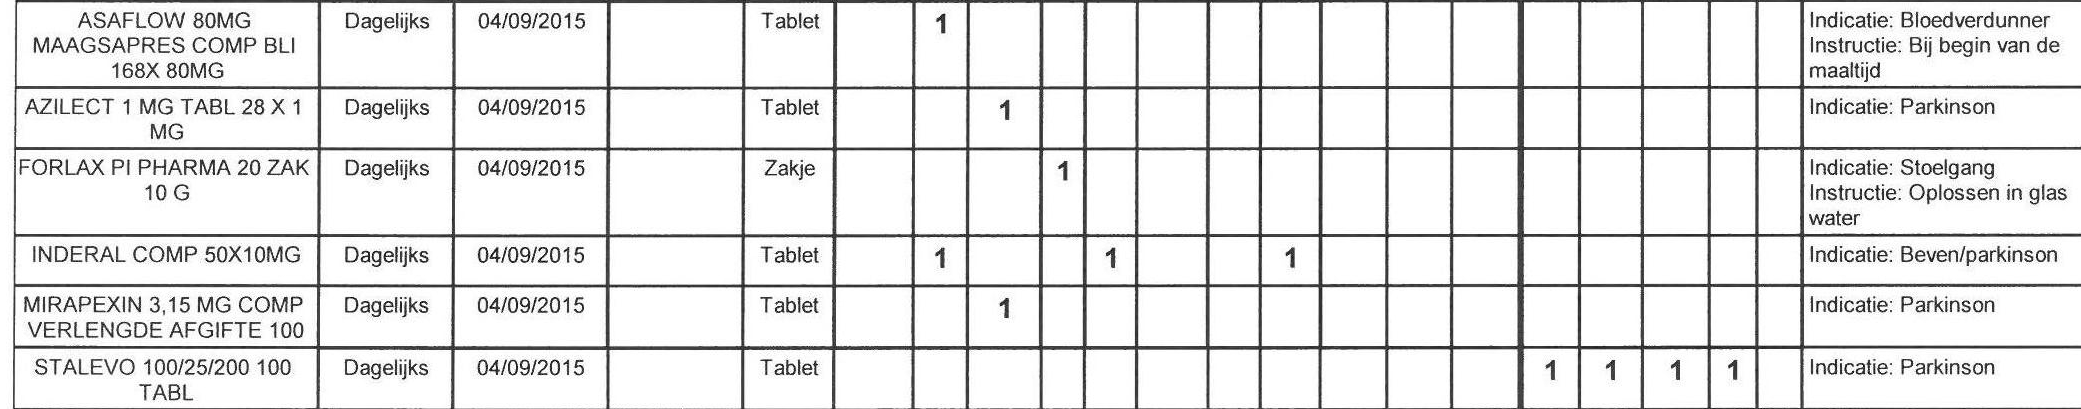
\includegraphics[width=1\textwidth]{img/lijn_detectie_origineel.png}
    \caption{Origineel geïsoleerd tabel.}
    \label{fig:lijn-detectie-origineel}
\end{figure}

In algoritme A, om de horizontale en verticale scheidingslijnen van de tabel te detecteren, wordt in een eerste stap, adaptive thresholding toegepast. Bij simpele thresholding wordt een afbeelding in kleur gesegmenteerd, meestal tot een zwart-wit-versie van de afbeelding. Indien de intensiteit van een pixel, bij simpele thresholding, een vaste threshold (drempelwaarde) overschrijdt, wordt de pixel als zwart gesegmenteerd, anders als wit. Bij adaptive thresholding is de waarde van de threshold afhankelijk van de regio waarin de pixel zich bevindt. In de volgende figuur werd adaptive thresholding toegepast op de origineel figuur \ref{fig:lijn-detectie-origineel}.

\begin{figure}[H]
    \centering
    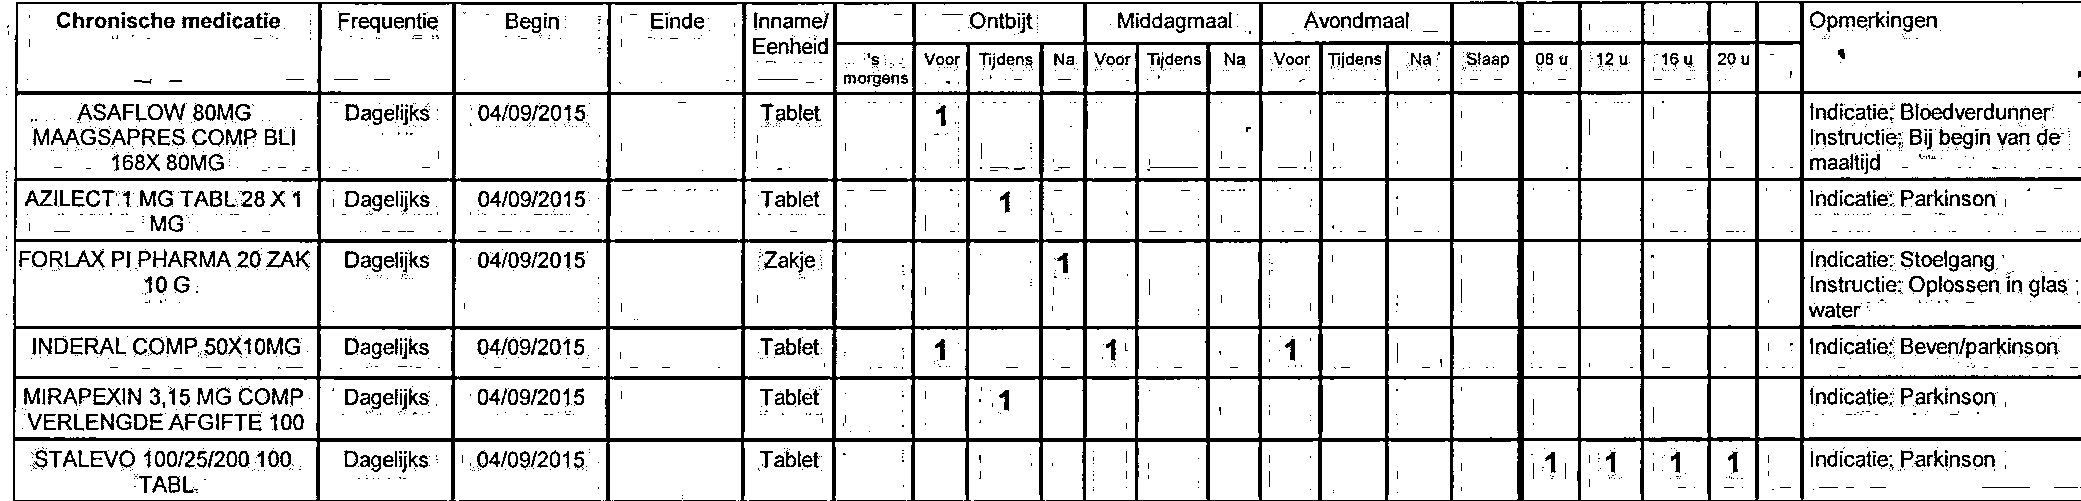
\includegraphics[width=1\textwidth]{img/line_detection_a_1_adaptive_threshold_on_image.png}
    \caption{Adaptive thresholding.}
\end{figure}

Vervolgens wordt een bitwise-not-operatie uitgevoerd. Dit heeft als gevolg dat de kleuren geïnverteerd worden.

\begin{figure}[H]
    \centering
    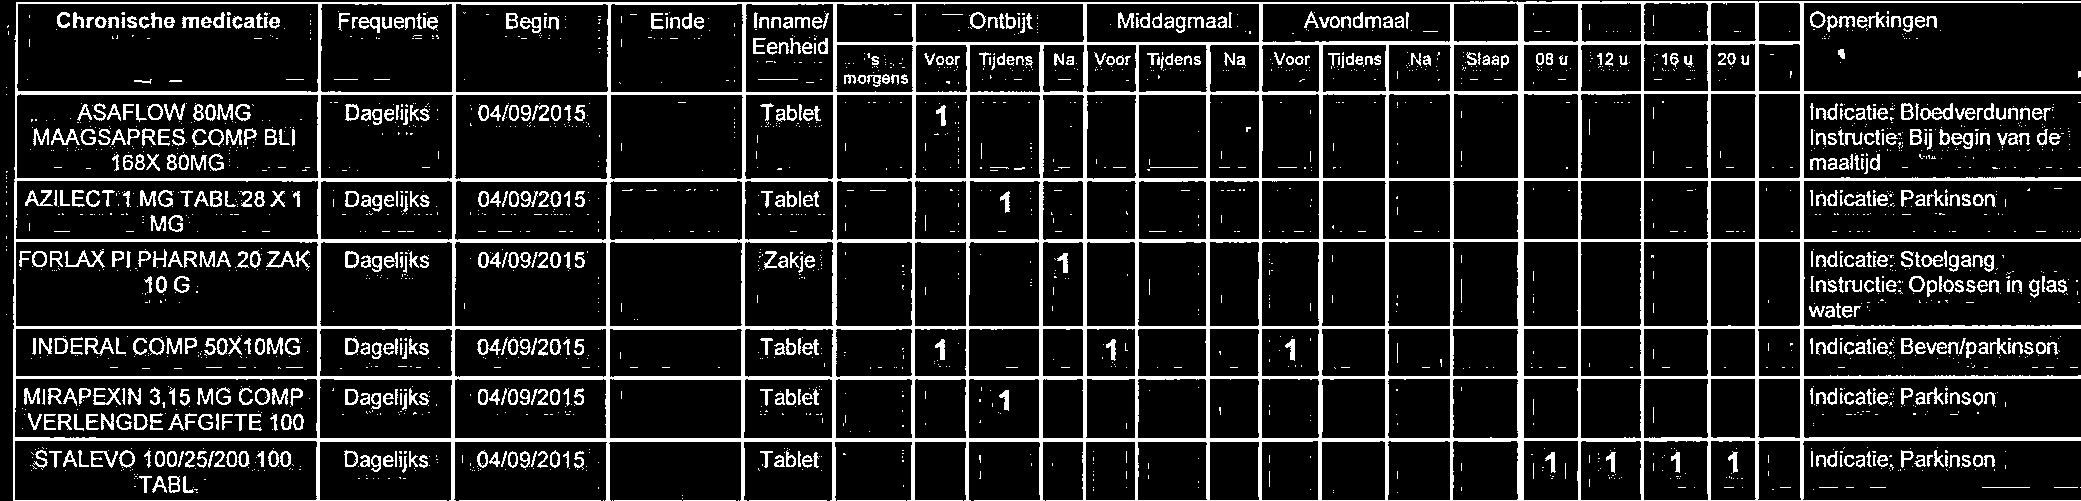
\includegraphics[width=1\textwidth]{img/line_detection_a_2_bitwise_not_on_image.png}
    \caption{Bitwise-not-operatie.}
\end{figure}

Hierna, om horizontale lijnen te detecteren, worden de pixels geërodeerd d.m.v. een horizontale structuur.

\begin{figure}[H]
    \centering
    
\includegraphics[width=1\textwidth]{img/line_detection_a_3_erode_horizontal_structure_for_horizontal_lines.png}
    \caption{Erosie d.m.v. een horizontale structuur.}
\end{figure}

Nadien vindt een dilatatie van de pixels plaats, d.m.v. de horizontale structuur.

\begin{figure}[H]
    \centering
    
\includegraphics[width=1\textwidth]{img/line_detection_a_4_dilate_horizontal_structure_for_horizontal_lines.png}
    \caption{Dilatatie d.m.v. de horizontale structuur.}
\end{figure}

Hierna wordt een simpele dilatatie uitgevoerd, gevolgd door een simpele erosie.

\begin{figure}[H]
    \centering
    
\includegraphics[width=1\textwidth]{img/line_detection_a_5_dilate_image_for_horizontal_lines.png}
    \caption{Simpele dilatatie.}
\end{figure}

\begin{figure}[H]
    \centering
    
\includegraphics[width=1\textwidth]{img/line_detection_a_6_erode_image_for_horizontal_lines.png}
    \caption{Simpele erosie.}
\end{figure}

Uiteindelijk worden horizontale structuren met een te kleine lengte buiten beschouwing gebracht en wordt een Hough Line-transformatie uitgevoerd. Zo worden de horizontale lijnen verkregen. Op een analoog manier worden de verticale lijnen gedetecteerd. De gedetecteerde lijnen zijn in figuur \ref{fig:lines-detected-a} in rood en groen voorgesteld.

\begin{figure}[H]
    \centering
    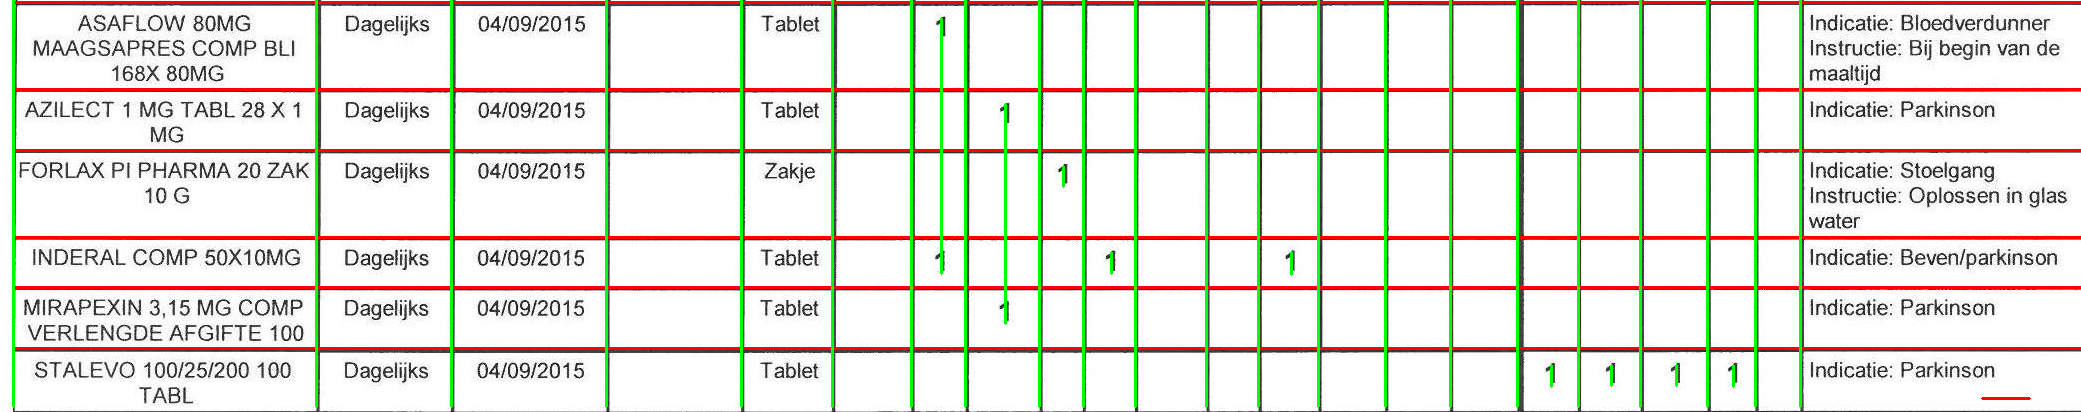
\includegraphics[width=1\textwidth]{img/lines_detected_a.png}
    \caption{Lijnen gedetecteerd door algoritme A.}
    \label{fig:lines-detected-a}
\end{figure}

Met algoritme B wordt een andere aanpak voor de lijnendetectie voorgesteld.

Zo worden eerst de tekstblokken, gedetecteerd door \Gls{OCR}, gemaskeerd door witte rechthoeken om de tekstelementen binnen de tabel te verbergen. In de volgende figuur \ref{fig:line-detection-b-text-removed} wordt het resultaat van deze operatie weergegeven. Men kan merken dat er nog tekstelementen aanwezig zijn. Dit komt omdat de resolutie van de ingescande document laag is, waardoor de \Gls{OCR}-software niet alle tekstblokken heeft kunnen detecteren.

\begin{figure}[H]
    \centering
    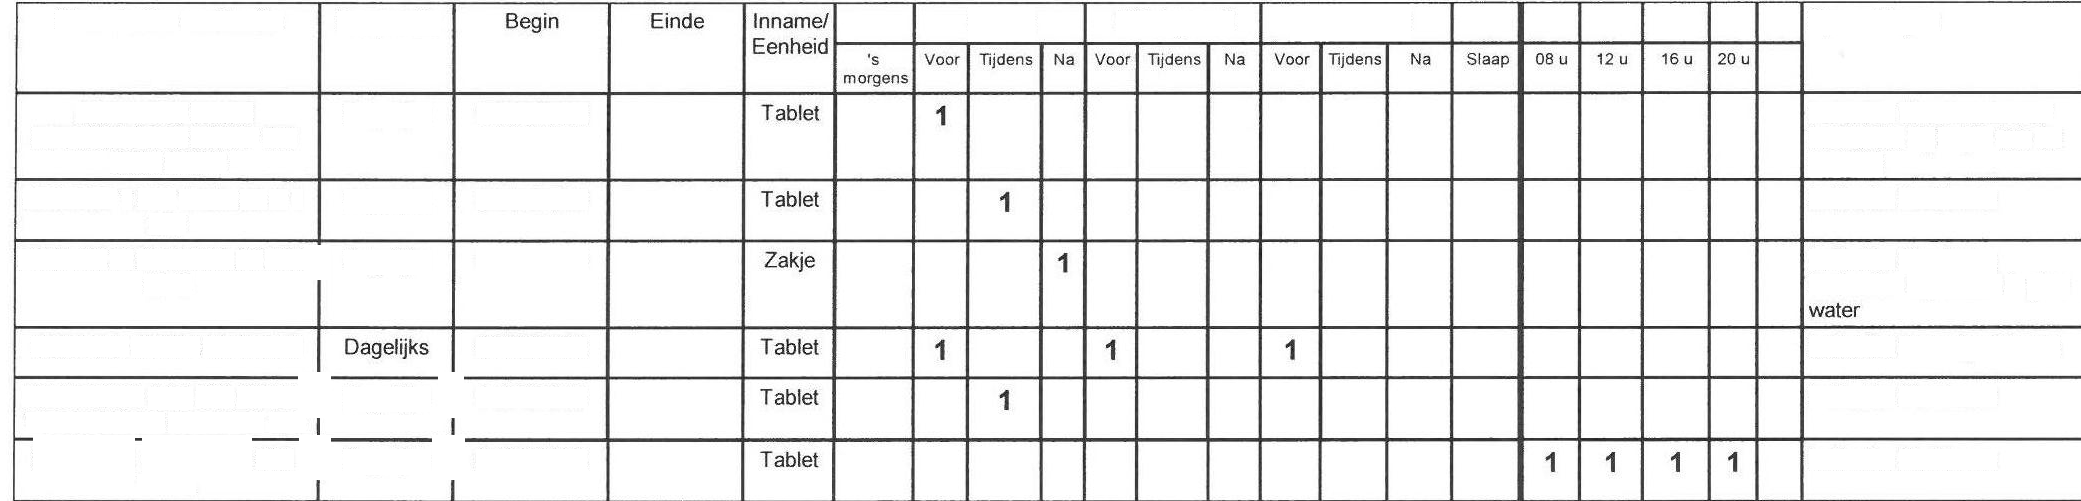
\includegraphics[width=1\textwidth]{img/line_detection_b_1_detected_text_removed.png}
    \caption{Verwijdering van tekstelementen.}
    \label{fig:line-detection-b-text-removed}
\end{figure}

Vervolgens wordt een dilatatie, gevolgd door een erosie uitgevoerd.

\begin{figure}[H]
    \centering
    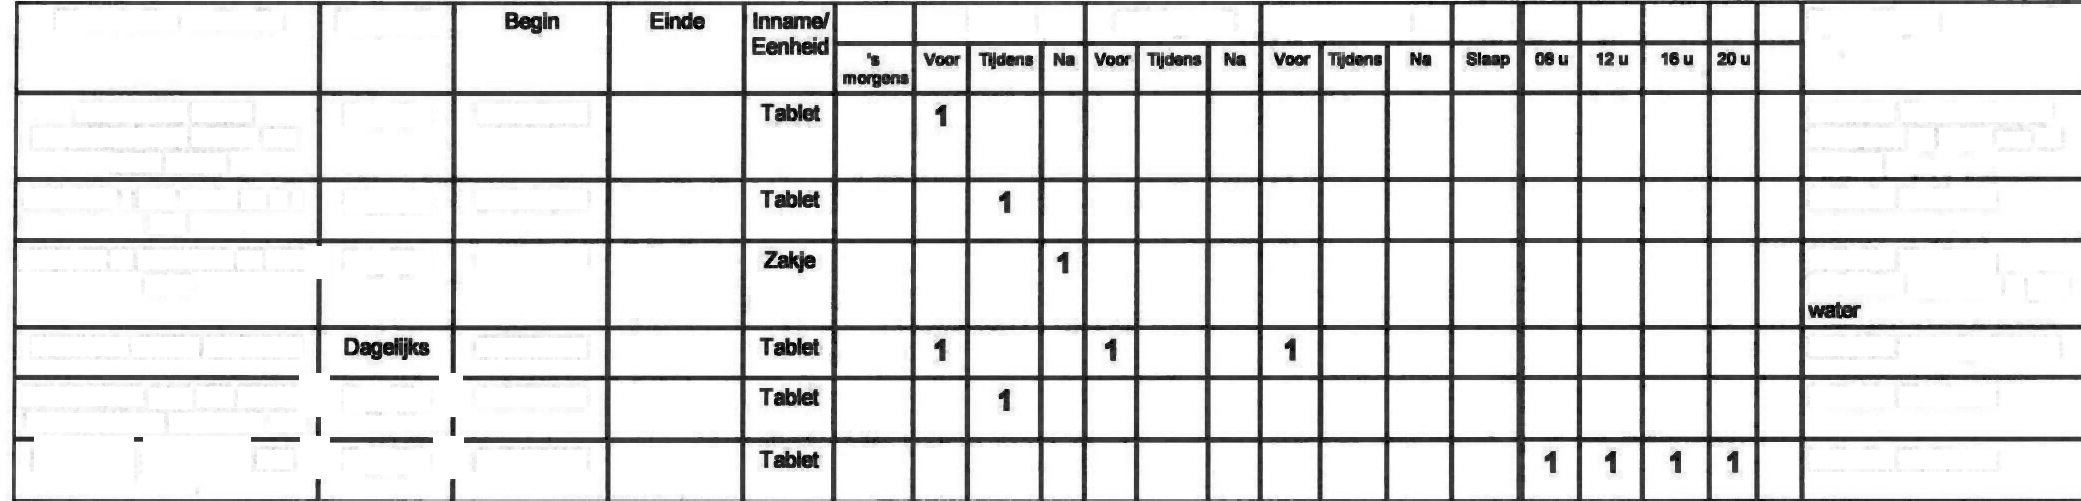
\includegraphics[width=1\textwidth]{img/line_detection_b_2_image_eroded.png}
    \caption{Dilatatie.}
\end{figure}

\begin{figure}[H]
    \centering
    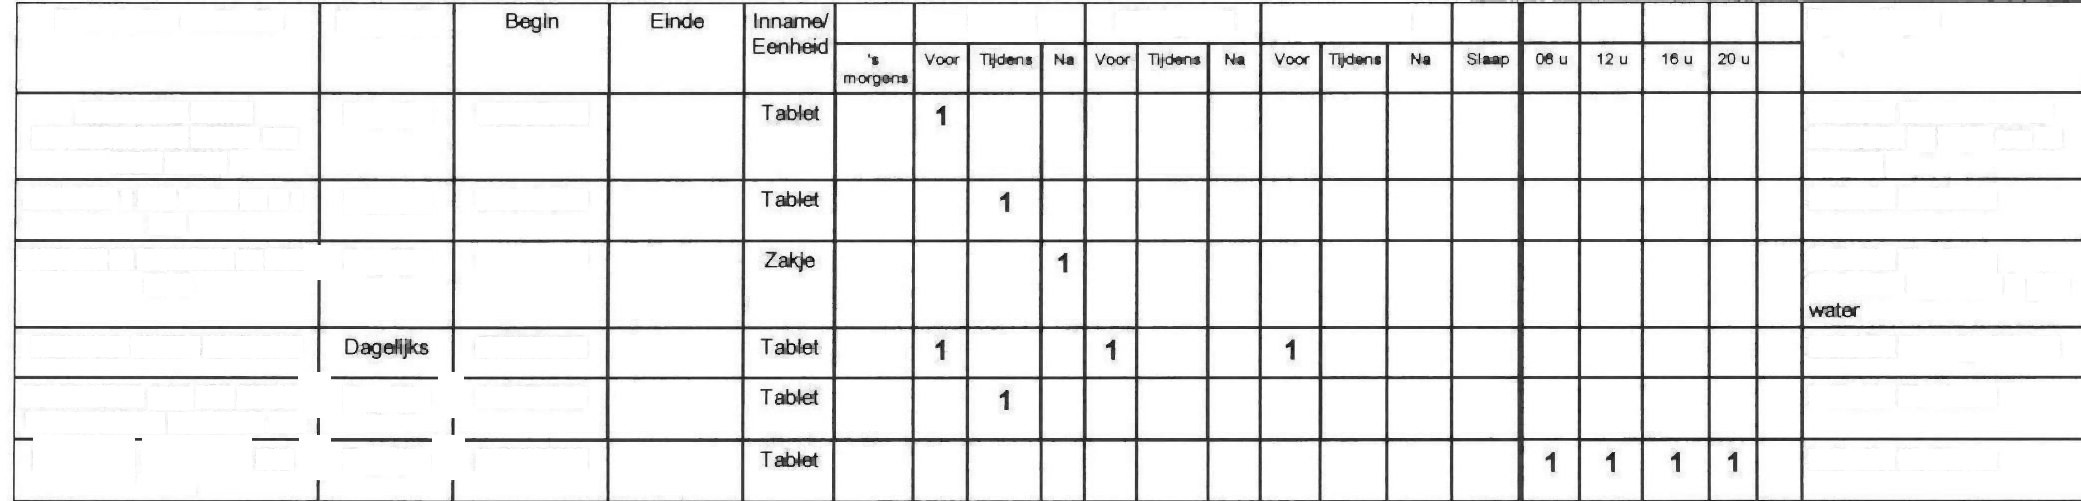
\includegraphics[width=1\textwidth]{img/line_detection_b_3_image_dilated.png}
    \caption{Erosie.}
\end{figure}

Uiteindelijk worden een Canny edge-operatie en een Hough-Line-transformatie toegepast om de horizontale en verticale tegelijk te detecteren. Deze gedetecteerde lijnen zijn in figuur \ref{fig:lines-detected-b} in rood en groen voorgesteld.

\begin{figure}[H]
    \centering
    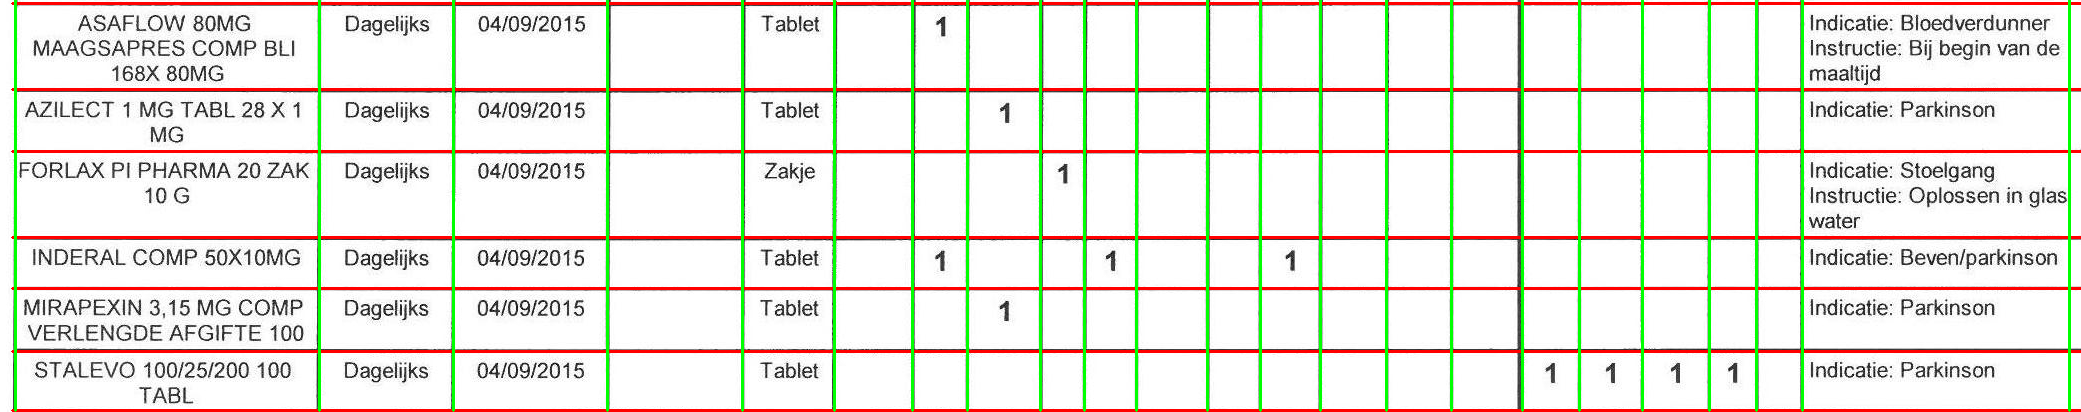
\includegraphics[width=1\textwidth]{img/lines_detected_b.png}
    \caption{Lijnen gedetecteerd door algoritme B.}
    \label{fig:lines-detected-b}
\end{figure}

Met de volgende figuren \ref{fig:lines-detected-a} en \ref{fig:lines-detected-b} wordt het resultaat van beide algoritmes opnieuw weergegeven.

\begin{figure}[H]
    \centering
    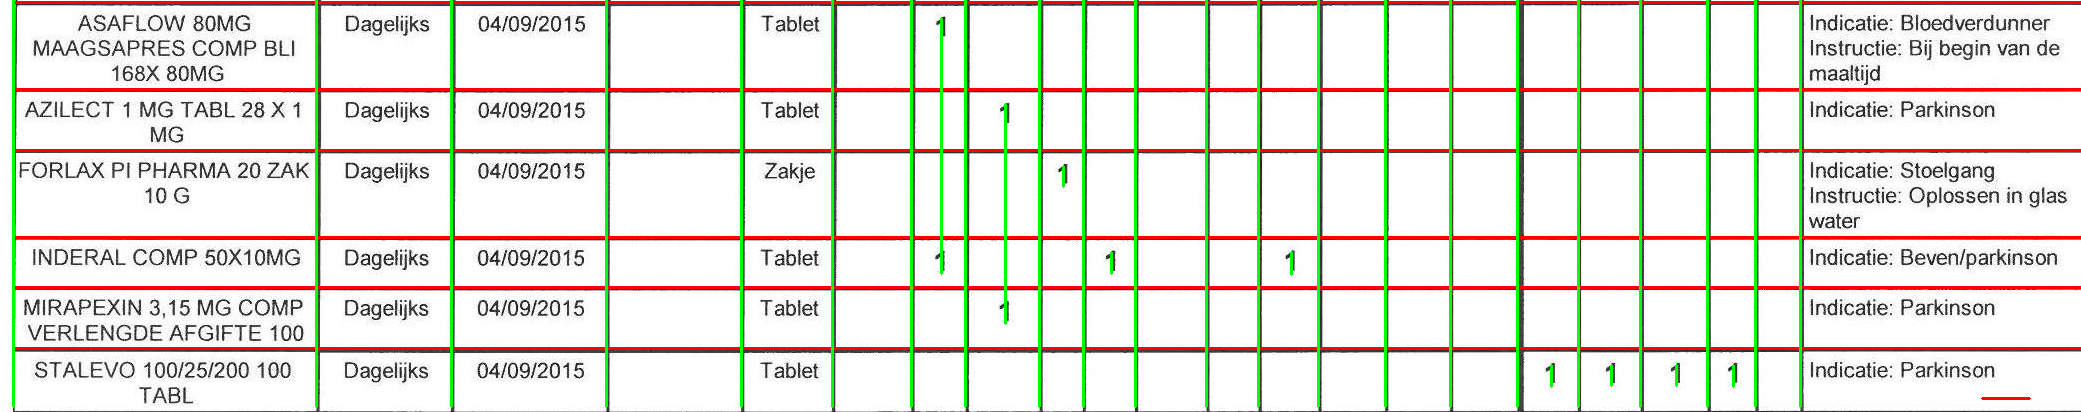
\includegraphics[width=1\textwidth]{img/lines_detected_a.png}
    \caption{Lijnen gedetecteerd door algoritme A.}
    \label{fig:lines-detected-a-overzicht}
\end{figure}

\begin{figure}[H]
    \centering
    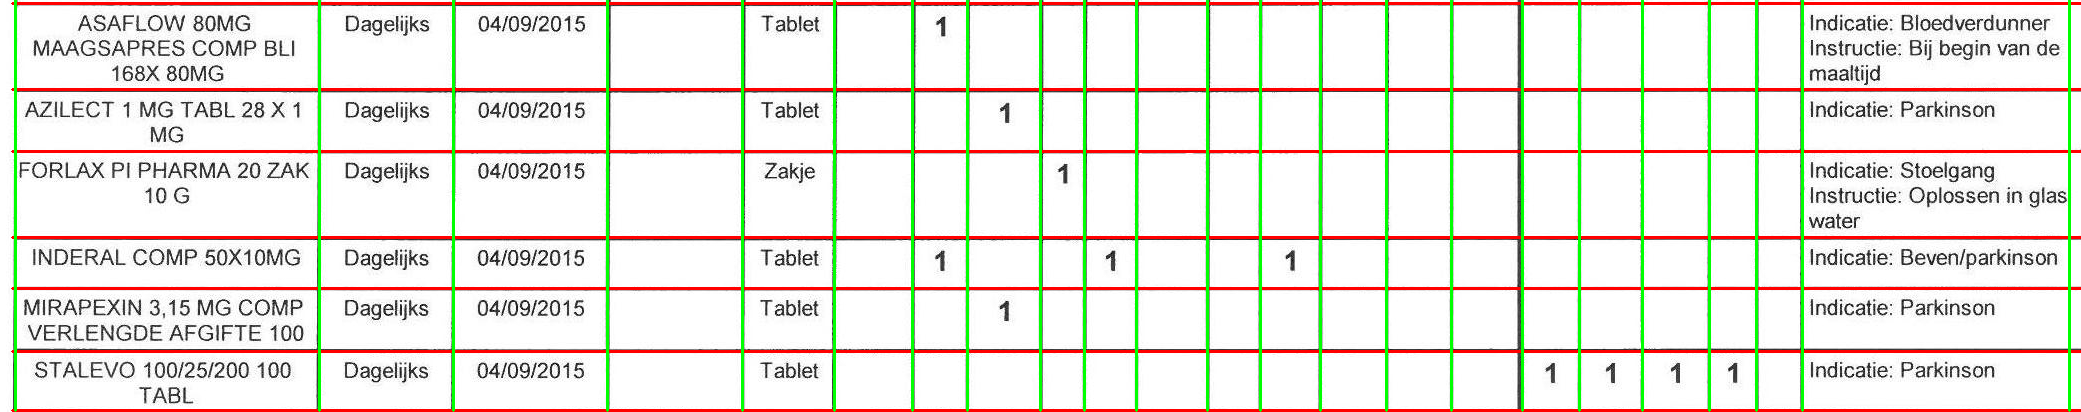
\includegraphics[width=1\textwidth]{img/lines_detected_b.png}
    \caption{Lijnen gedetecteerd door algoritme B.}
    \label{fig:lines-detected-b-overzicht}
\end{figure}

Zoals men kan zien, heeft algoritme A last van valse positieven. Er worden namelijk teveel lijnen gedetecteerd. Dit komt enerzijds omdat het de streep van de tekstelementen ``1`` als verticale lijnen detecteerd. Anderzijds wordt door afbeeldingruis een extra horizontaal lijn, rechts onderaan, gedetecteerd. Met algoritme B worden alle lijnen correct gedetecteerd.

Voor borderless tabellen wordt een clusteringalgoritme voorgesteld, in combinatie met lijndetectie.

\subsection{Postprocessing}
\label{subsec:post-processing}

Aangezien algoritme B op \Gls{OCR} steunt voor tabelstructuuranalyse, is een postprocessing van het resultaat noodzakelijk. Postprocessing is niet nodig indien gebruik gemaakt wordt van algoritme A.

Eens een Pandas Dataframe, met daarin tekstelementen met bijhorende rij- en kolomwaarden, verkregen is d.m.v. algoritme B, vindt concatenatie plaats. Hierbij worden tekstblokken die dezelfde rij- en kolomwaarden hebben, aan elkaar geconcateneerd. Bovendien worden volledige lege rijen en kolommen verwijderd van de Pandas Dataframe.

\subsection{Resultaatweergave}
\label{subsec:resultaat-weergave}

Na de strucuuranalyse, en postprocessing indien algoritme A gebruikt werd, wordt de Pandas Dataframe omgezet in een JSON-object die teruggestuurd wordt van de back end naar de GUI van de gebruiker. De gebruiker krijgt dan het resultaat van de tabeltransformatie te zien.

\begin{figure}[H]
    \centering
    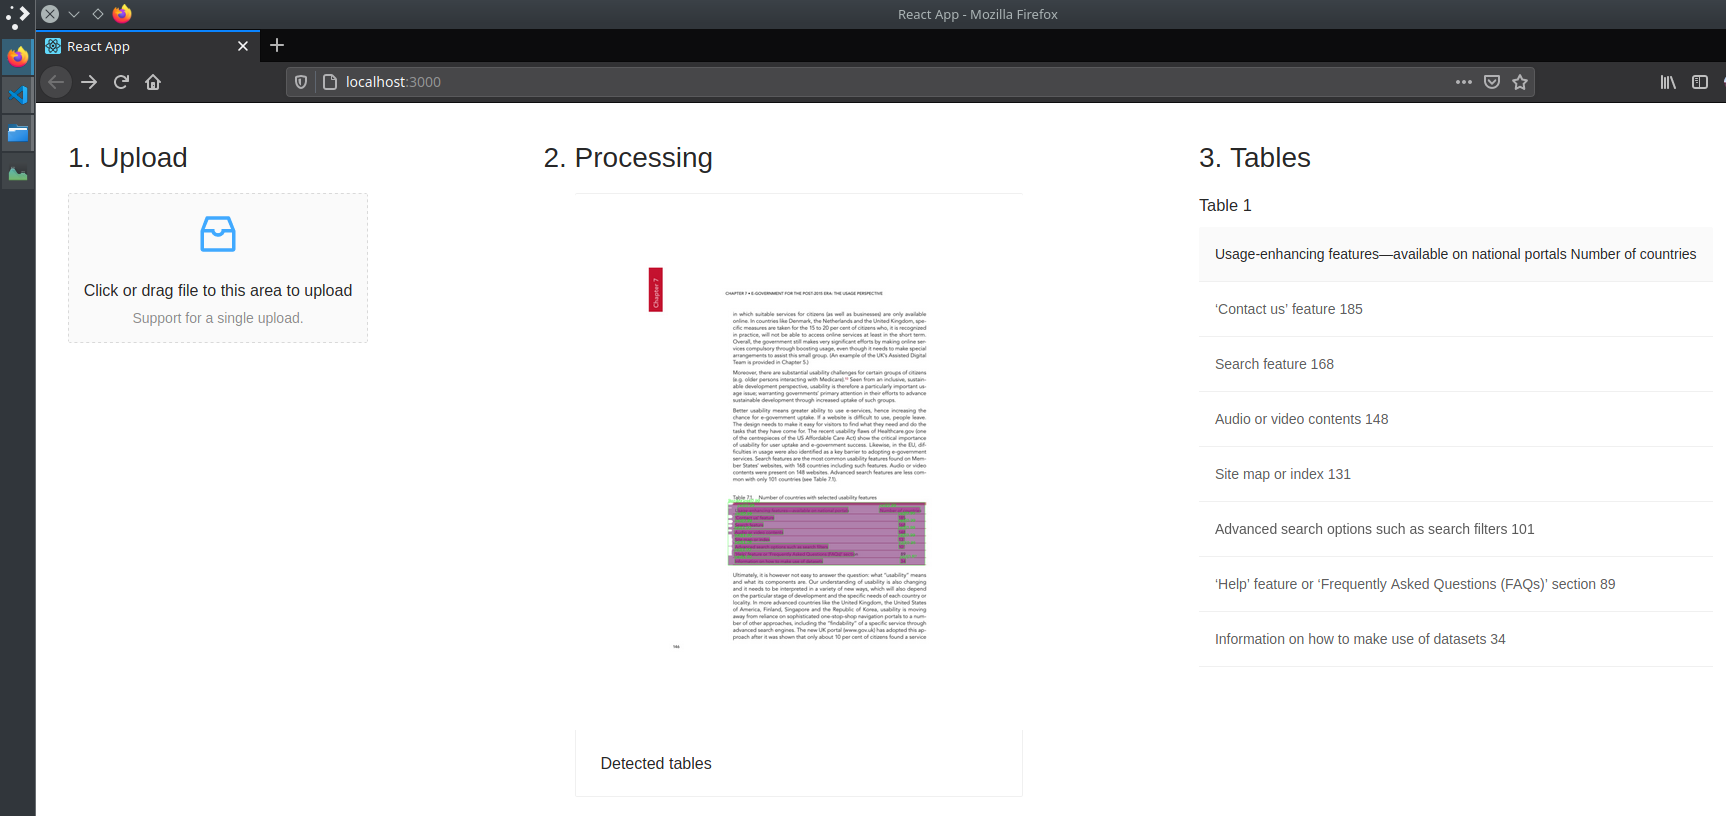
\includegraphics[width=1\textwidth]{img/gui_screenshot_used.png}
    \caption{GUI van de software wanneer de tabeltransformatie uitgevoerd is.}
    \label{fig:gui-screenshot-used}
\end{figure}

\section{Praktisch gebruik}
\label{sec:praktisch-gebruik}

\subsection{Hardware- en software-vereisten}
\label{subsec:hardware-en-software-vereisten}

Wat hardware betreft, is een grafische kaart van het merk NVIDIA nodig. Dit komt omdat, voor de tabeldetectie, \textcite{Prasad2020} gebruik maakt van een verouderd versie van MMDetection \autocite{Chen2019}, een objectdetectie-library. Bij de meest recente versie van MMDetection is objectdetectie d.m.v. enkel de CPU mogelijk. 

Wat software betreft is een Linux-distributie of MacOS nodig voor de tabeldetectie, aangezien MMDetection niet ondersteund wordt op het besturingssysteem Windows. Indien de tabellen reeds geïsoleerd zijn en dus enkel tabelstructuuranalyse nodig is, dan is tabeldetectie niet nodig en kan de software eveneens op Windows gebruikt worden.

\subsection{Installatie en gebruik}
\label{subsec:installatie-en-gebruik}

De open source broncode, inclusief gedetailleerde installatie- en gebruiksinstructies zijn te vinden in de repository \textcite{Nazari2020}.

%%=============================================================================
%% Resultaten
%%=============================================================================

\chapter{Resultaten}
\label{ch:resultaten}

Kijkend naar de resultaten van de tabeltransformatie van de dertig willekeurige documenten, die in \ref{ch:details-van-resultaten} bekeken kunnen worden, kan men enkele waarnemeingen maken. Zo ziet men dat \Gls{OCR} niet altijd nauwkeurig werkt, zeker niet wanneer de resolutie van de afbeelding laag is. Verder kan men merken dat de nauwkeurigheid van de tabeltransformatie afhankelijk is van de algoritme die gebruikt wordt voor tabelstructuuranalyse. Bij gebruik van de voorgestelde algoritme B is de slaagkans op een succesvolle tabeltransformatie merklijk groter dan indien algoritme A gebruikt zou worden.

% %%=============================================================================
%% Optimalisaties
%%=============================================================================

\chapter{Optimalisatiemogelijkheden}
\label{ch:optimalisatiemogelijkheden}


\section{Domeinkennis}
\label{sec:domeinkennis}

% Fuzzy search voor velden


\section{Natural Language Processing}
\label{sec:natural-language-processing}

% spellingsfouten, context


\section{Anomaliedetectie}
\label{sec:anomaliedetectie}


%%=============================================================================
%% Conclusie
%%=============================================================================

\chapter{Conclusie}
\label{ch:conclusie}

% TODO: Trek een duidelijke conclusie, in de vorm van een antwoord op de
% onderzoeksvra(a)g(en). Wat was jouw bijdrage aan het onderzoeksdomein en
% hoe biedt dit meerwaarde aan het vakgebied/doelgroep? 
% Reflecteer kritisch over het resultaat. In Engelse teksten wordt deze sectie
% ``Discussion'' genoemd. Had je deze uitkomst verwacht? Zijn er zaken die nog
% niet duidelijk zijn?
% Heeft het onderzoek geleid tot nieuwe vragen die uitnodigen tot verder 
%onderzoek?

Uit dit onderzoek kan men enkele conclusies trekken. Zo kan men, uit de literatuurstudie (hoofdstuk \ref{ch:stand-van-zaken}) concluderen dat tabeltransformatie een complex domein is. Kant en klaar software-pakketten voor tabeltransformatie bestaan, echter zijn deze niet open source en betalend. Een open source versie bestaat momenteel niet.

Verder kan men besluiten dan tabeltransformatie niet een simpel eenvoudig proces is, maar een complex procedure die uit verschillende subprocessen bestaat. Zo vindt preprocessing eerst plaats. Hierna wordt met tabeldetectie de tabellen van de rest van het document geïsoleerd. Vervolgens vindt de transformatie plaats d.m.v. structuuranalyse en \Gls{OCR}. Hierna wordt het resultaat verder behandeld door postprocessing. Uiteindelijk wordt de getransformeerd tabel terug naar de gebruiker gestuurd.

Bovendien kan men de gevolgtrekking maken dat, afhankelijk van de gebruikte algoritmes, pre- en postprocessing ofwel noodzakelijk ofwel niet nodig zijn. Voor de proof-of-concept, bij gebruik van de voorgestelde algoritme, is postprocessing bijvoorbeeld noodzakelijk. Postprocessing bleek in het algemeen nodig te zijn voor de proof-of-concept, om nauwkeurig tabellen te kunnen detecteren.

Tenslotte kan men concluderen dat tabeldetectie enerzijds zeer nauwkeurig is, terwijl anderzijds structuuranalyse minder optimale resultaten kan leveren. De algoritme voorgesteld in dit onderzoek, die een niet onbelangrijke verbetering van de tabeltransformaties heeft teweeggebracht, toont aan dat optimalisatiemogelijkheden zeker nog mogelijk zijn.


%%=============================================================================
%% Bijlagen
%%=============================================================================

\appendix
\renewcommand{\chaptername}{Appendix}

%%=============================================================================
%% Resultaten details
%%=============================================================================

\chapter{Details van resultaten}
\label{ch:details-van-resultaten}

\newpage

\section{Document 1}

\begin{figure}[H]
    \centering
    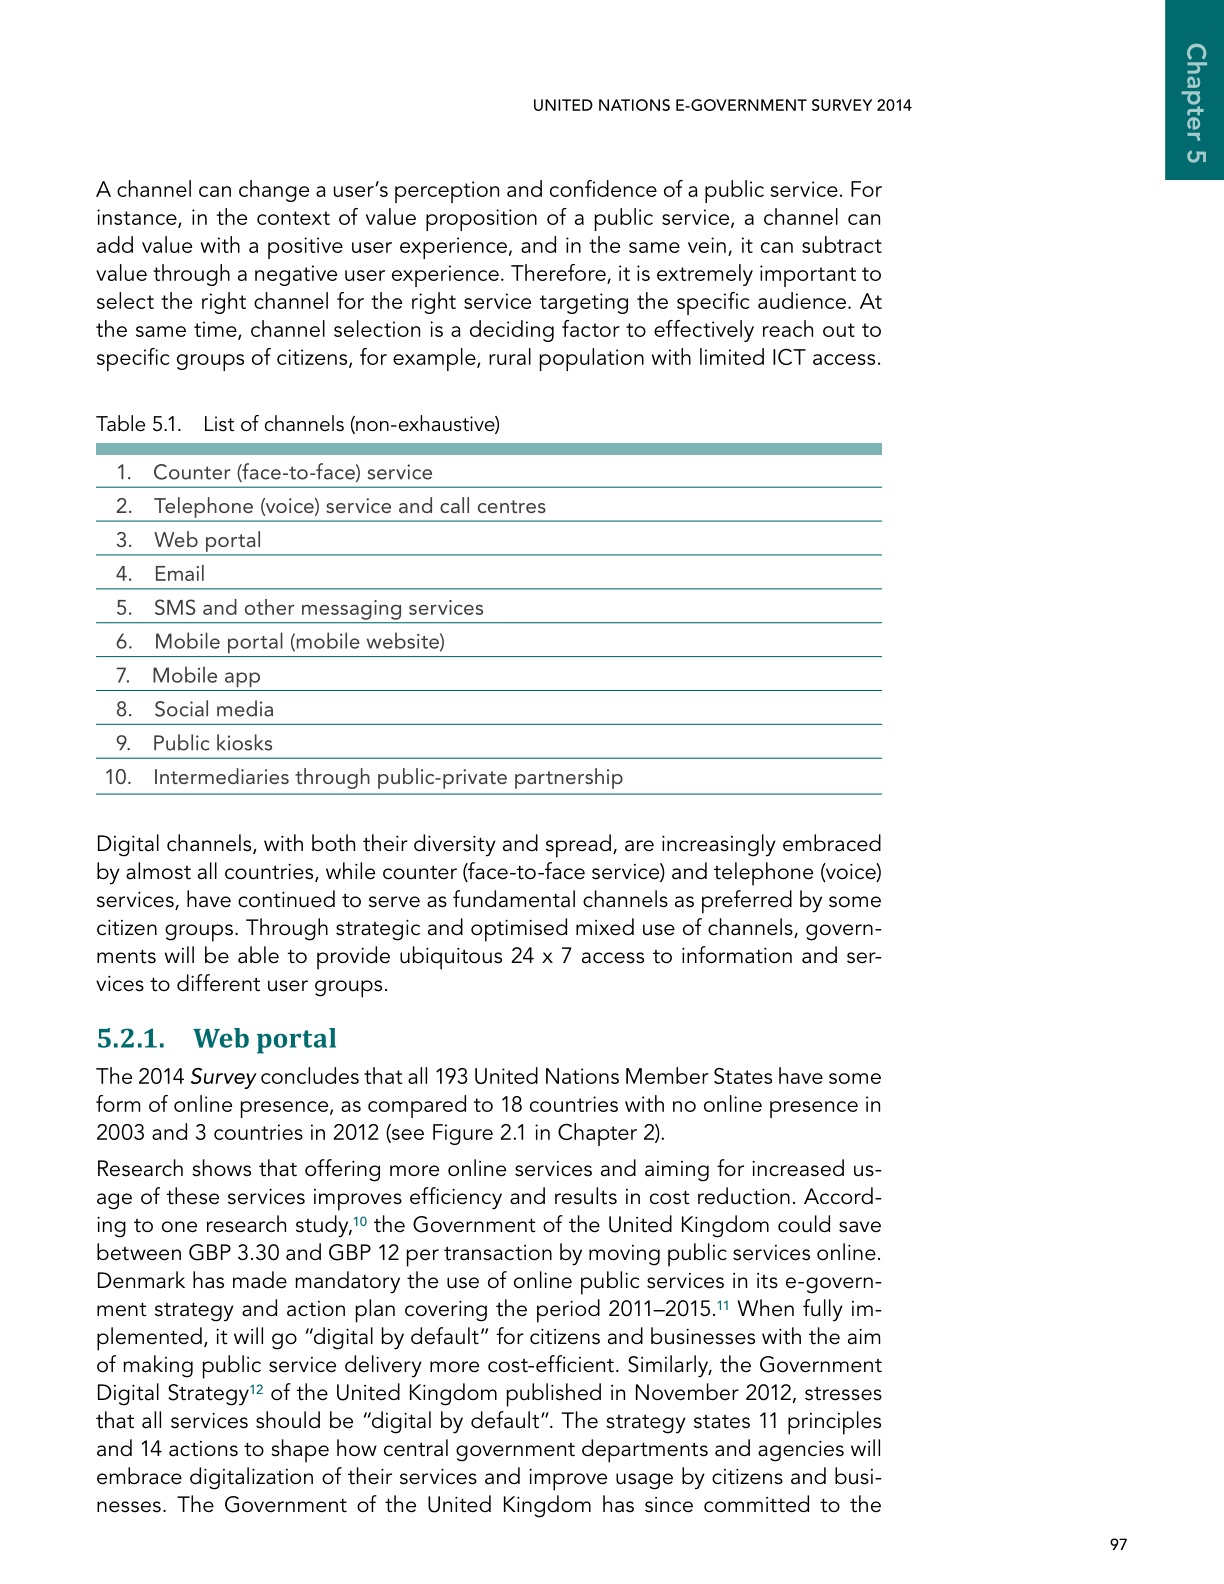
\includegraphics[width=0.8\textwidth]{test-resultaten/1/original.jpg}
    \caption{Origineel document.}
\end{figure}

\begin{figure}[H]
    \centering
    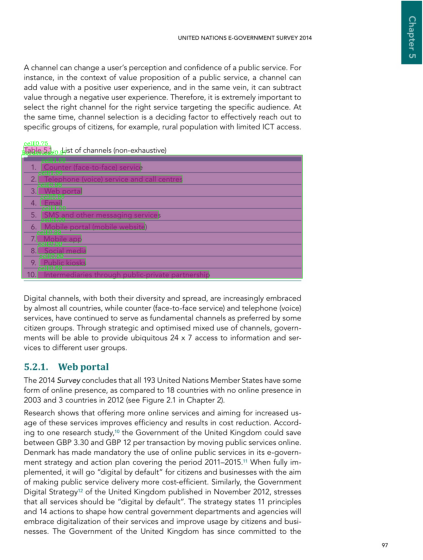
\includegraphics[width=0.8\textwidth]{test-resultaten/1/detected_tables.png}
    \caption{Gedetecteerde tabellen.}
\end{figure}

Getransformeerde tabellen met algoritme A:

\begin{tabular}{ll}
\toprule
{} &                     Counter (face-to-face) service \\
\midrule
0 &         Telephone (voice) service and call centres \\
1 &                                         Web portal \\
2 &                                               Emai \\
3 &                   SMS and other messaging service: \\
4 &                      Mobile portal (mobile website \\
5 &                                      7. Mobile apo \\
6 &                                       Social media \\
7 &                                      Public kiosks \\
8 &  Intermediaries through public-private partnershir \\
\bottomrule
\end{tabular}

Getransformeerde tabellen met algoritme B:

\begin{tabular}{ll}
\toprule
{} &                  1. Counter (face-to-face) service \\
\midrule
0 &      2. Telephone (voice) service and call centres \\
1 &                                      3. Web portal \\
2 &                                           4. Email \\
3 &                5. SMS and other messaging services \\
4 &                  6. Mobile portal (mobile website) \\
5 &                                      7. Mobile app \\
6 &                                    8. Social media \\
7 &                                   9. Public kiosks \\
8 &  10. Intermediaries through public-private part... \\
\bottomrule
\end{tabular}

\section{Document 2}

\begin{figure}[H]
    \centering
    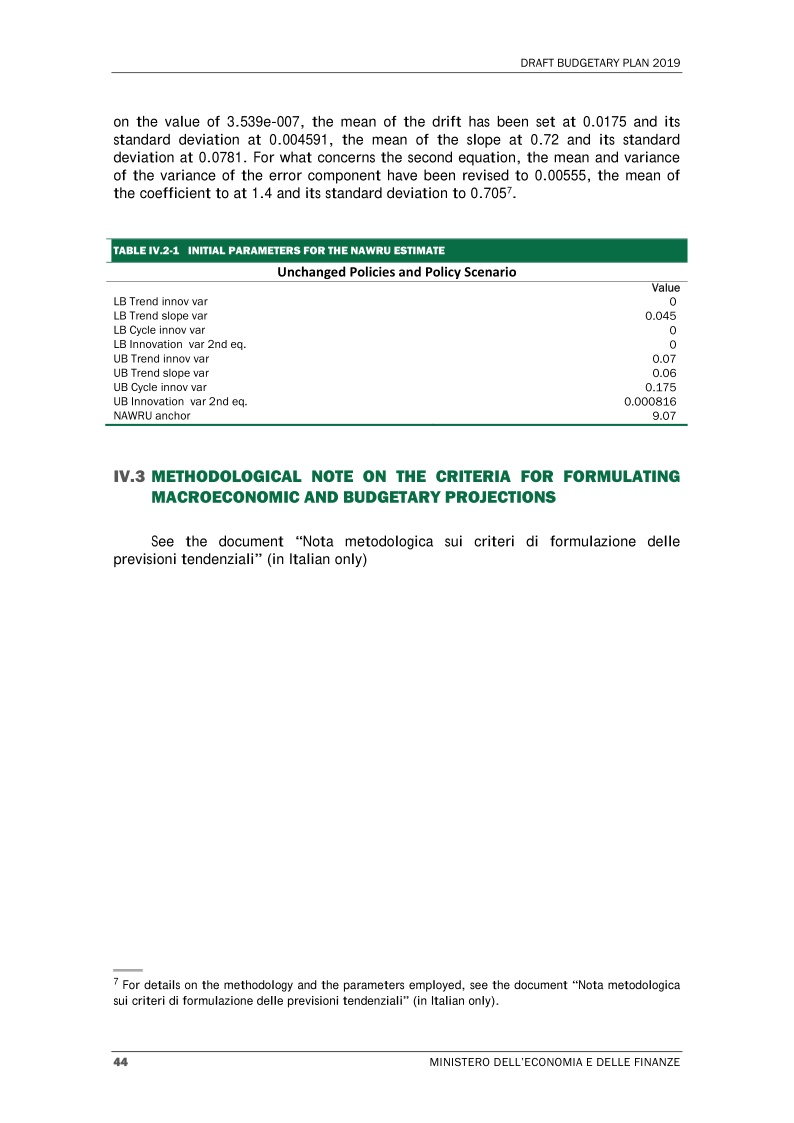
\includegraphics[width=0.8\textwidth]{test-resultaten/2/original.jpg}
    \caption{Origineel document.}
\end{figure}

\begin{figure}[H]
    \centering
    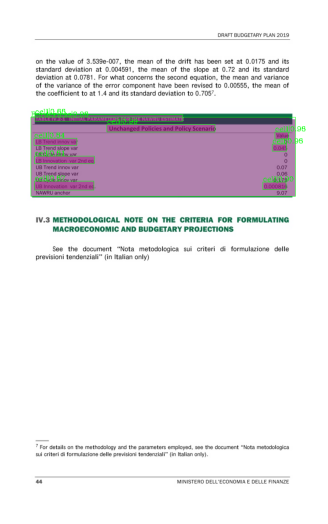
\includegraphics[width=0.8\textwidth]{test-resultaten/2/detected_tables.png}
    \caption{Gedetecteerde tabellen.}
\end{figure}

Getransformeerde tabellen met algoritme A:

Tabeltransformatie gefaald.

Getransformeerde tabellen met algoritme B:

\begin{tabular}{lll}
\toprule
{} &                      ate haath alee eid &       NaN \\
\midrule
0  &  Unchanged Policies and Policy Scenario &      None \\
1  &                                    None &      Vane \\
2  &                      L8 Trend innov var &        90 \\
3  &                      LB Trend slope var &     0.045 \\
4  &                       LB Cycle inno var &         0 \\
5  &               LB Innovation var 2nd ea, &         0 \\
6  &                      UB Trend Innov var &       O07 \\
7  &                      UB Trend stope var &      0.08 \\
8  &                      UB Cycle innov var &     0.178 \\
9  &               UB Innovation var 2nd ea, &  0.000816 \\
10 &                            NAWRU anchor &     ‘9.07 \\
\bottomrule
\end{tabular}
\section{Document 3}

\begin{figure}[H]
    \centering
    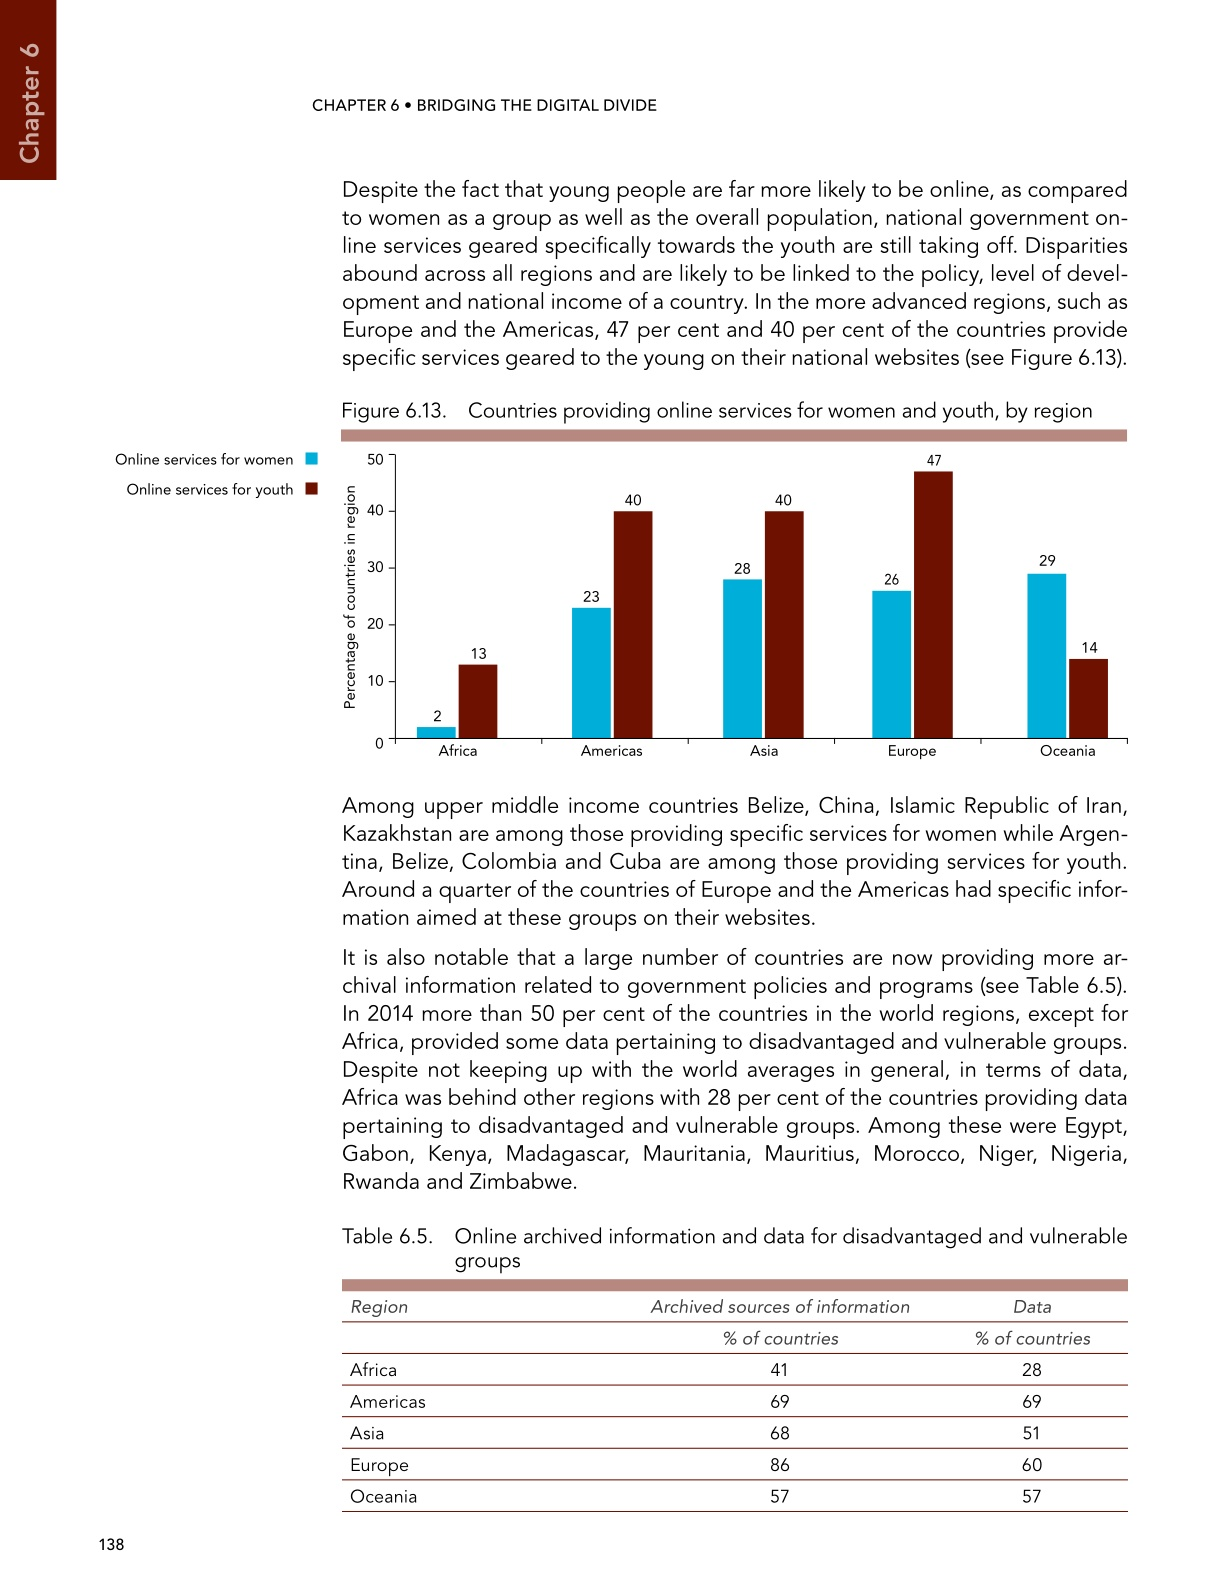
\includegraphics[width=0.8\textwidth]{test-resultaten/3/original.jpg}
    \caption{Origineel document.}
\end{figure}

\begin{figure}[H]
    \centering
    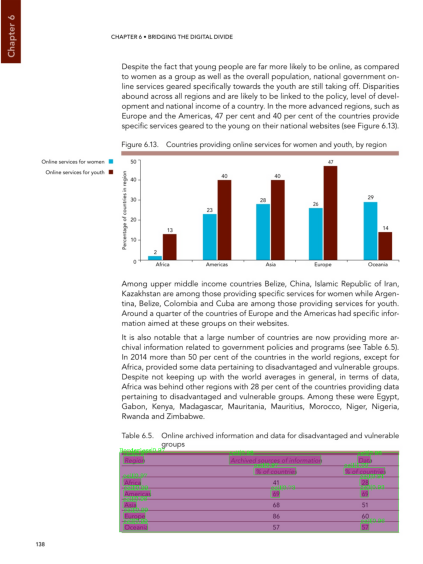
\includegraphics[width=0.8\textwidth]{test-resultaten/3/detected_tables.png}
    \caption{Gedetecteerde tabellen.}
\end{figure}

Getransformeerde tabellen met algoritme A:

\begin{tabular}{llll}
\toprule
{} &          Region & Archived sources of information &  Data \\
\midrule
0 &  \% of countries &                  \% of countries &  None \\
1 &          Africa &                              Al &    28 \\
2 &        Americas &                              69 &    69 \\
3 &            Asia &                              68 &    51 \\
4 &          Europe &                              Bb &    60 \\
5 &         Oceania &                              57 &    57 \\
\bottomrule
\end{tabular}

Getransformeerde tabellen met algoritme B:

\begin{tabular}{llll}
\toprule
{} &    Region & Archived sources of information &            Data \\
\midrule
0 &      None &                  \% of countries &  \% of countries \\
1 &    Africa &                               A &              28 \\
2 &  Americas &                              69 &              69 \\
3 &      Asia &                              68 &              51 \\
4 &    Europe &                              86 &              60 \\
5 &   Oceania &                              57 &              a7 \\
\bottomrule
\end{tabular}

\section{Document 4}

\begin{figure}[H]
    \centering
    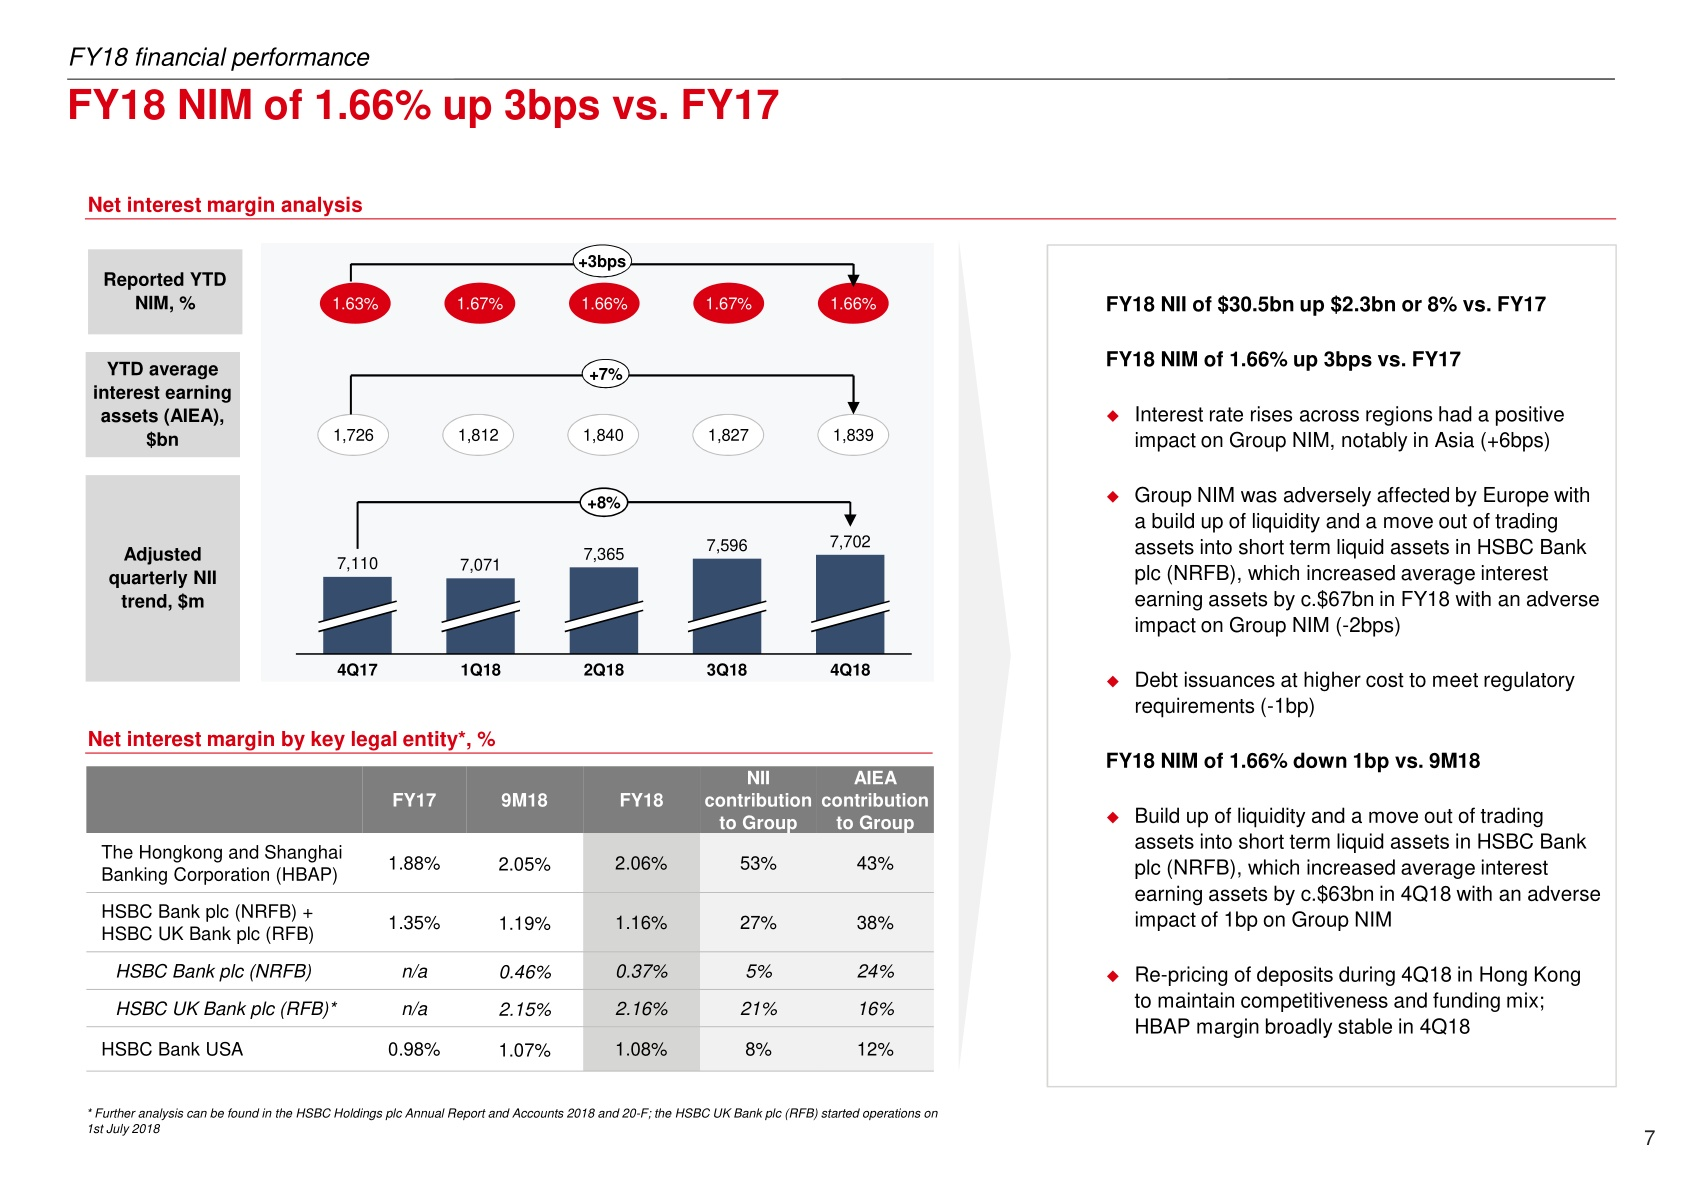
\includegraphics[width=0.8\textwidth]{test-resultaten/4/original.jpg}
    \caption{Origineel document.}
\end{figure}

\begin{figure}[H]
    \centering
    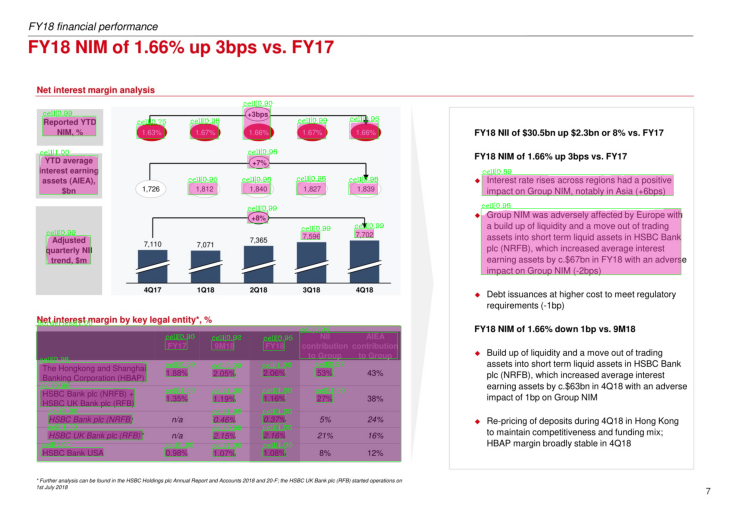
\includegraphics[width=0.8\textwidth]{test-resultaten/4/detected_tables.png}
    \caption{Gedetecteerde tabellen.}
\end{figure}

Getransformeerde tabellen met algoritme A:

Tabeltransformatie gefaald.

Getransformeerde tabellen met algoritme B:

\begin{tabular}{lllllll}
\toprule
{} &                      The Hongkong and Shanghai &  1.88\% &  2.05\% &  2.06\% &    53\% &      43\% \\
\midrule
0 &                     Banking Corporation (HBAP) &   None &   None &   None &   None &     None \\
1 &  HSBC Bank ple (NRFB) + HSBC UK Bank ple (RFB) &  1.35\% &  1.19\% &  1.16\% &    27\% &      38\% \\
2 &                           HSBC Bank plc (NRFB) &     Wa &  0.46\% &  0.37\% &     5\% &      24\% \\
3 &                        HSBC UK Bank plo (RFB)* &     na &  2.15\% &  2.16\% &    21\% &      16\% \\
4 &                                  HSBC Bank USA &  0.98\% &  1.07\% &  1.08\% &     8\% &      12\% \\
5 &                                           None &   FY17 &    ey) &    aly &   Pele &  mr hel) \\
6 &                                           None &   None &   None &   None &    ii\} &       rN \\
7 &                                           None &   None &   None &   None &  eect) &   feeds) \\
\bottomrule
\end{tabular}
\section{Document 5}

\begin{figure}[H]
    \centering
    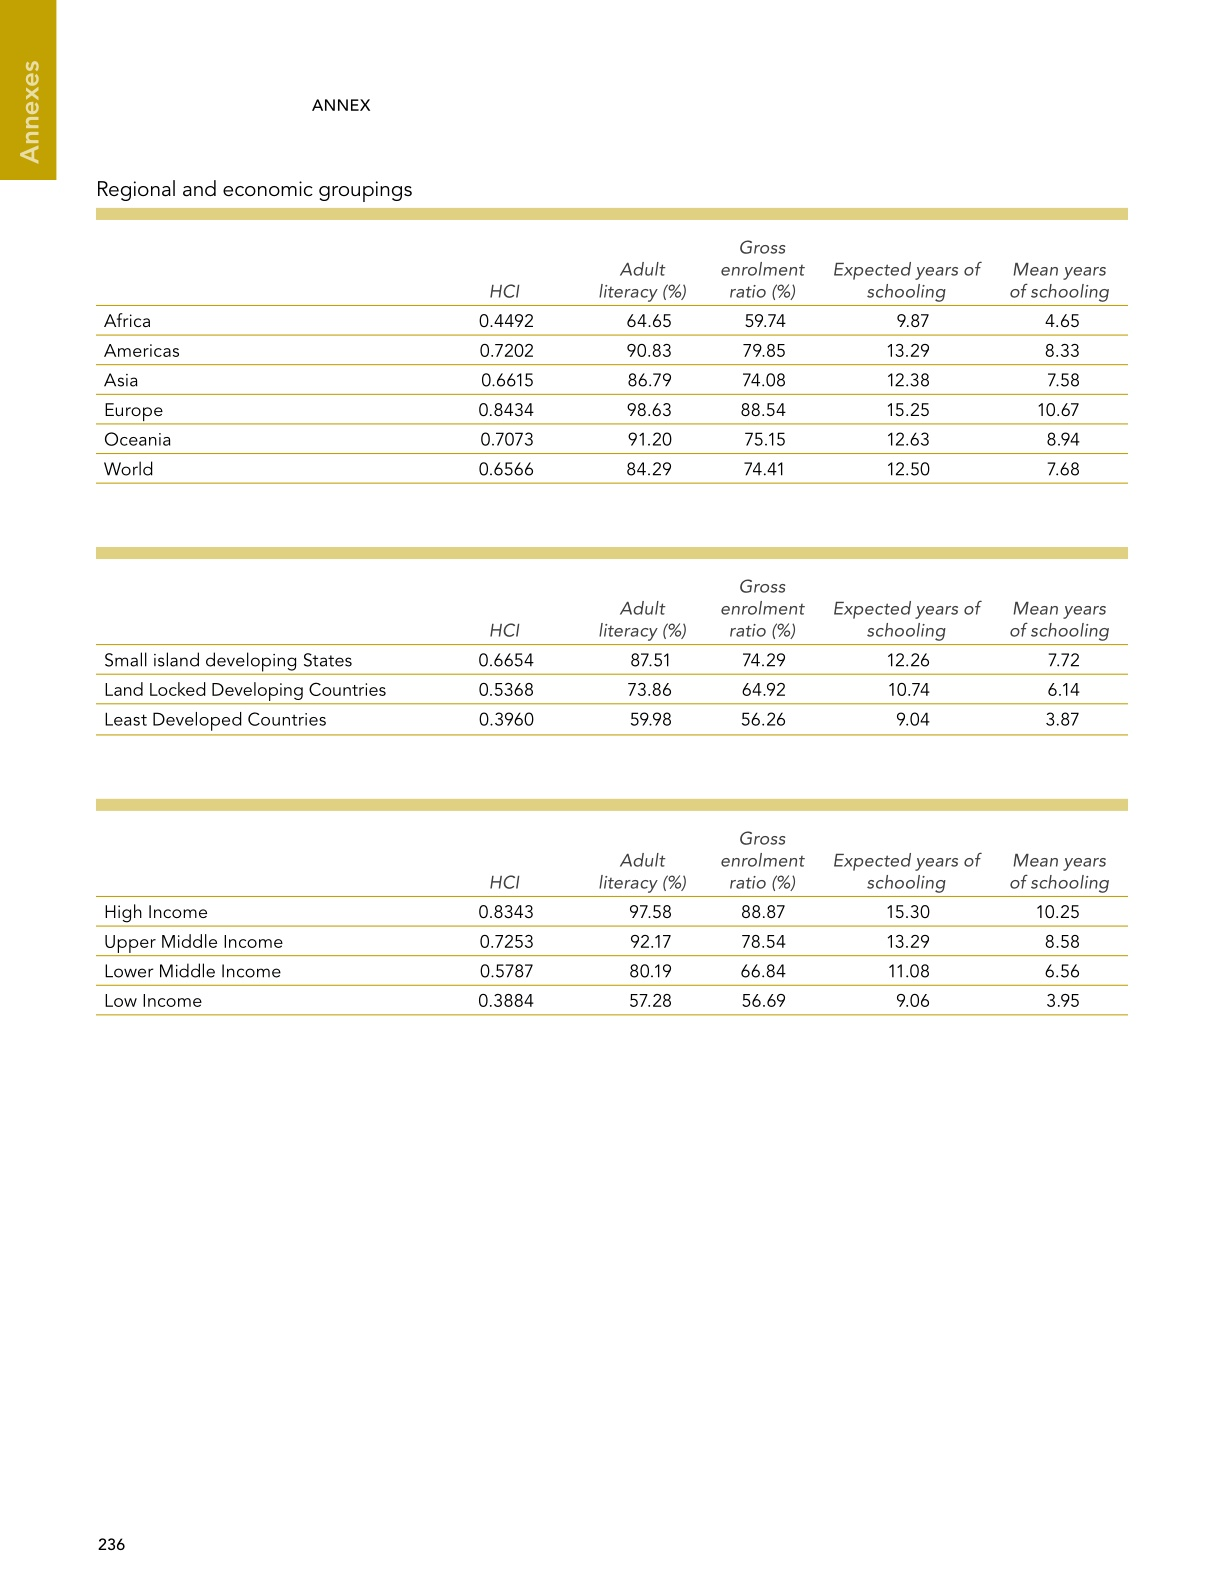
\includegraphics[width=0.8\textwidth]{test-resultaten/5/original.jpg}
    \caption{Origineel document.}
\end{figure}

\begin{figure}[H]
    \centering
    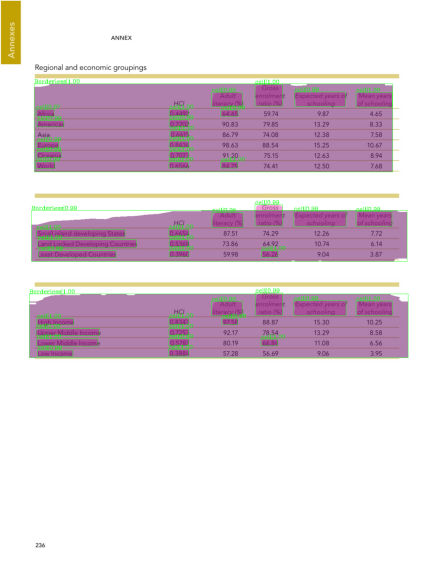
\includegraphics[width=0.8\textwidth]{test-resultaten/5/detected_tables.png}
    \caption{Gedetecteerde tabellen.}
\end{figure}

Getransformeerde tabellen met algoritme A:

\begin{tabular}{lllll}
\toprule
{} & Adult\textbackslash nliteracy (\% & Gross\textbackslash nenrolmen\textbackslash nratio (\%) & Expected years of\textbackslash nschooling & Mean years\textbackslash nof schooling \\
\midrule
0 &             Africa &                      59.74 &                          987 &                      465 \\
1 &           Americas &                      79.85 &                        13.29 &                     8.33 \\
2 &              06615 &                      74.08 &                        12.38 &                     7.58 \\
3 &             Europe &                      88.54 &                        15.25 &                    10.67 \\
4 &            Oceania &                      75.15 &                        12.63 &                      894 \\
5 &              World &                      74.41 &                        12.50 &                     7.68 \\
\bottomrule
\end{tabular}

\begin{tabular}{lllll}
\toprule
{} &  Adult\textbackslash nliteracy (\%, & Gross\textbackslash nenrolment\textbackslash nratio (\%) & Expected years of\textbackslash nschooling & Mean years\textbackslash nof schooling \\
\midrule
0 &          High Income &                       88.87 &                        15.30 &                    10.25 \\
1 &  Upper Middle Income &                       78.54 &                        13.29 &                     8.58 \\
2 &  Lower Middle Incom: &                       66.84 &                        11.08 &                     6.56 \\
3 &           Low Income &                       56.69 &                         9.06 &                      395 \\
\bottomrule
\end{tabular}

\begin{tabular}{lllll}
\toprule
{} &               Adult\textbackslash nliteracy (\%) & enrolment\textbackslash nratio (\%) & Expected years of\textbackslash nschooling & Mean years\textbackslash nof schooling \\
\midrule
0 &    Small island developing States &                74.29 &                        12.26 &                      772 \\
1 &  Land Locked Developing Countrie: &                64.92 &                        10.74 &                     6.14 \\
2 &         Least Developed Countries &                56.26 &                          904 &                       oF \\
\bottomrule
\end{tabular}

Getransformeerde tabellen met algoritme B:

\begin{tabular}{lllllll}
\toprule
{} &        Gross &           NaN &               NaN &           NaN &     NaN &       NaN \\
\midrule
0 &    enrolment &         Adult &  Expected yearsof &    Mean years &    None &      None \\
1 &  \_\_ratio (\%) &  literacy (\%) &         schooling &  of schooling &     HCI &      None \\
2 &        59.74 &         64.65 &              9.87 &          4.65 &  0.4492 &    Africa \\
3 &        79.85 &         90.83 &             13.29 &          8.33 &  0.7202 &  Americas \\
4 &        74.08 &         86.79 &             12.38 &          7.58 &  0.6615 &      Asia \\
5 &        88.54 &         98.63 &             18.25 &         10.67 &  0.8434 &    Europe \\
6 &        75.15 &         91.20 &             12.63 &          8.94 &  0.7073 &   Oceania \\
7 &         None &         84.29 &             12.50 &          7.68 &  0.6566 &     World \\
\bottomrule
\end{tabular}

\begin{tabular}{lllllll}
\toprule
{} &                     Gross &               NaN &           NaN &           NaN &     NaN &     NaN \\
\midrule
0 &           Adult enrolment &  Expected yearsof &    Mean years &          None &    None &    None \\
1 &  literacy (\%) \_ ratio (\%) &         schooling &  of schooling &          None &    None &    None \\
2 &               97.58 88.87 &             15.30 &         10.25 &   High Income &  0.8343 &    None \\
3 &               92.17 78.54 &             13.29 &          8.58 &  Upper Middle &  0.7253 &  Income \\
4 &               80.19 66.84 &             11.08 &          6.56 &  Lower Middle &  0.5787 &  Income \\
5 &               57.28 56.69 &              9.06 &          3.95 &    Low Income &  0.3884 &    None \\
\bottomrule
\end{tabular}

\begin{tabular}{llllll}
\toprule
{} &         Adult &   enrolment & Expected yearsaf © Mean years &     NaN &                               NaN \\
\midrule
0 &  literacy (\%) &  \_ratio (\%) &        schooling of schooling &     Het &                              None \\
1 &         87.51 &       74.29 &                     12.26 772 &  0.6654 &    Small island developing States \\
2 &         73.86 &       64.92 &                    10.74 6.14 &  0.5368 &  Land Locked Developing Countries \\
3 &         59.98 &       56.26 &                     9.04 3.87 &  0.3960 &         Least Developed Countries \\
\bottomrule
\end{tabular}
\section{Document 6}

\begin{figure}[H]
    \centering
    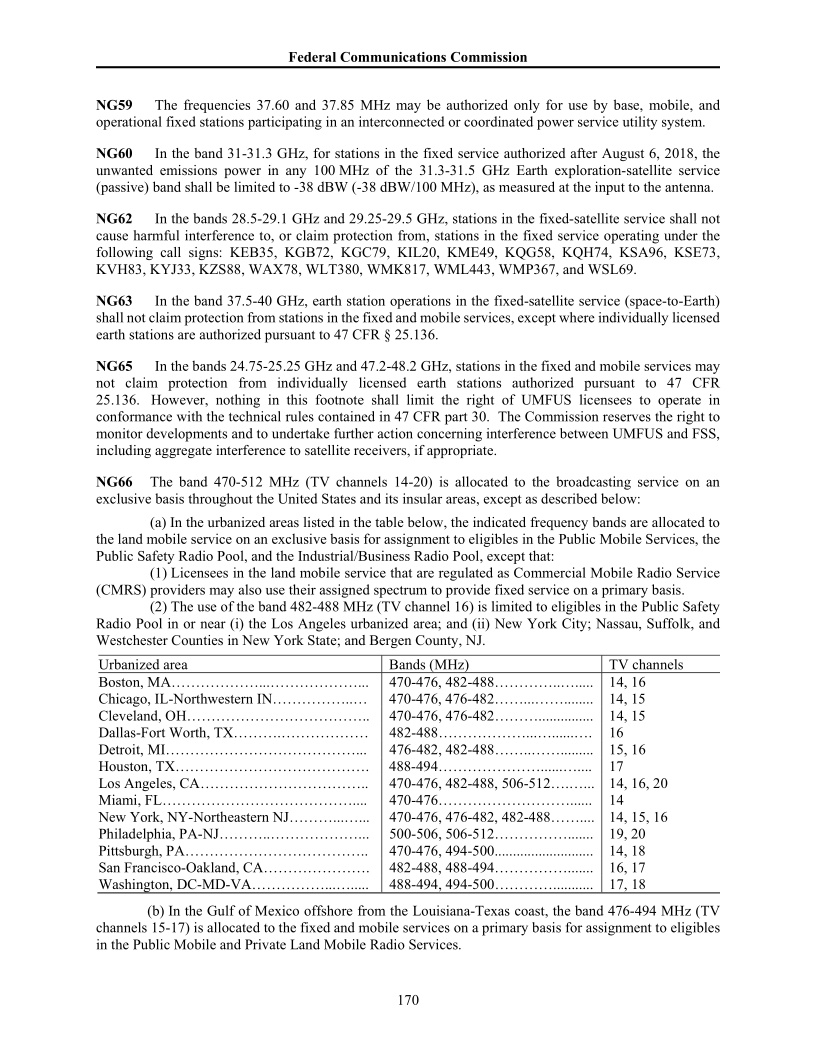
\includegraphics[width=0.8\textwidth]{test-resultaten/6/original.jpg}
    \caption{Origineel document.}
\end{figure}

\begin{figure}[H]
    \centering
    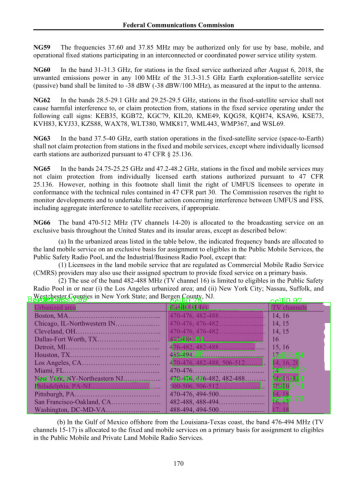
\includegraphics[width=0.8\textwidth]{test-resultaten/6/detected_tables.png}
    \caption{Gedetecteerde tabellen.}
\end{figure}

Getransformeerde tabellen met algoritme A:

\begin{tabular}{lll}
\toprule
{} &                                    ‘Urbanized area &                                        TV channels \\
\midrule
0 &  Dallas-Fort Worth, TX.\textbackslash n\textbackslash nDetroit, MI\textbackslash n\textbackslash nHoust... &  16\textbackslash n\textbackslash n15, 16\textbackslash n7\textbackslash n\textbackslash n14, 16.\textbackslash n14\textbackslash n\textbackslash n14,15\textbackslash n19, 2... \\
\bottomrule
\end{tabular}

Getransformeerde tabellen met algoritme B:

\begin{tabular}{llll}
\toprule
{} &                                 Urbanized area &                         Bands (MH) &   TV channels \\
\midrule
0  &                                  Boston, MA... &                  AT0-AT6, 482-488, &         14,16 \\
1  &                   Chicago, 1L-Northwestern IN. &                   410-476, 476-482 &          141s \\
2  &                               Cleveland, OH... &                470-476, 476-482... &        14,15, \\
3  &                         Dallas-Fort Worth, TX. &                           482-488, &            16 \\
4  &                                    Detroit, MI &                  476-482, 482-488. &         15,16 \\
5  &                                   Houston, TX. &                           488-494, &            17 \\
6  &                               Los Angeles, CA. &         470-476, 482-488, 506-512. &    14, 16, 20 \\
7  &  Miami. EL...... New York, NY-1 Northeastem NI &  AT0AT6, AT0AT6, 476-482, 482-488. &  14 14, 15,16 \\
8  &                           Philadelphia, PA-NJ. &                  500-506, 506-512. &        19, 20 \\
9  &                                Pittsburgh, PA. &                  470-476, 494-500, &         14.18 \\
10 &                      San Francisco-Oakland, €. &                  482-488, 488-494. &        16,17, \\
11 &                          Washington, DC-MD-VA. &                  488-494, 494-500. &        17,18, \\
\bottomrule
\end{tabular}
\section{Document 7}

\begin{figure}[H]
    \centering
    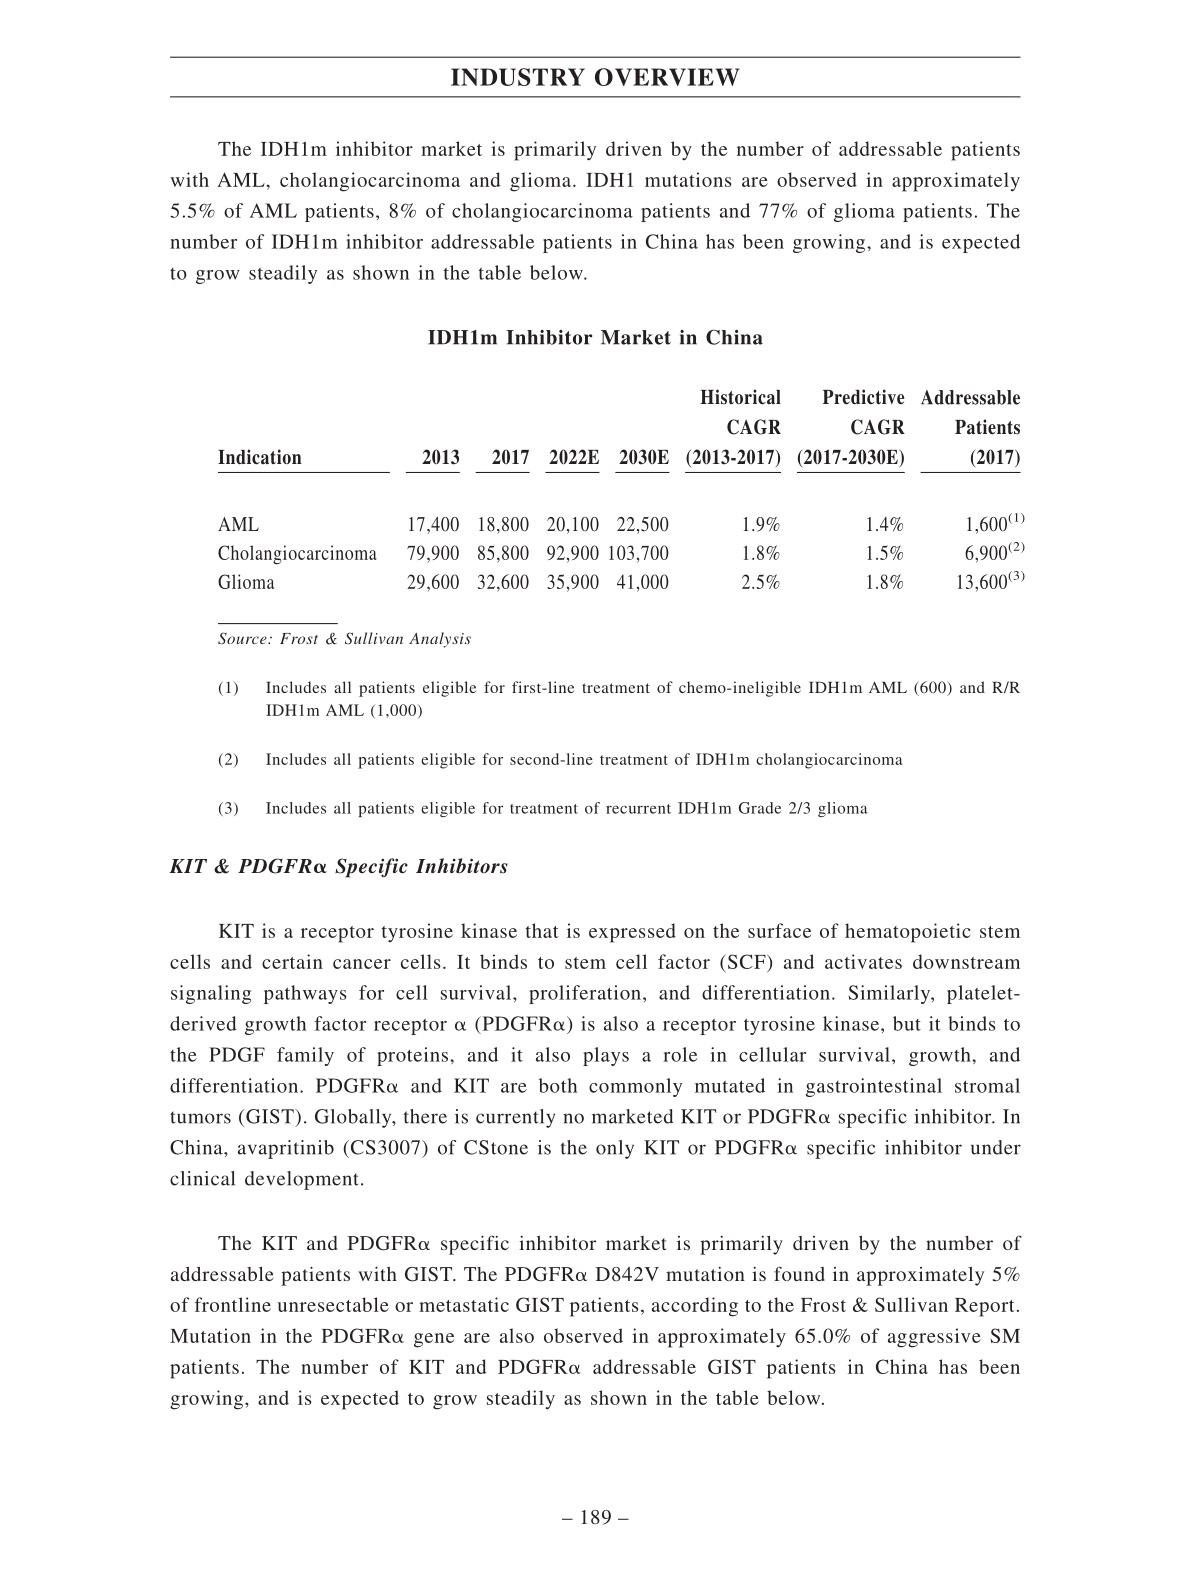
\includegraphics[width=0.8\textwidth]{test-resultaten/7/original.jpg}
    \caption{Origineel document.}
\end{figure}

\begin{figure}[H]
    \centering
    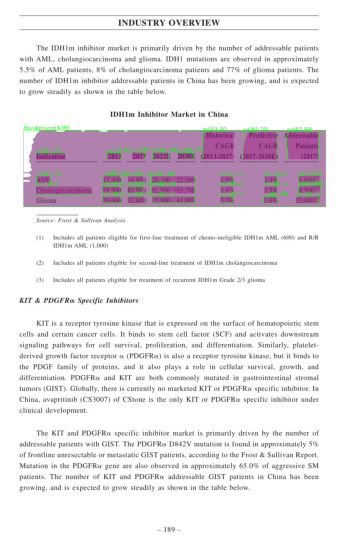
\includegraphics[width=0.8\textwidth]{test-resultaten/7/detected_tables.png}
    \caption{Gedetecteerde tabellen.}
\end{figure}

Getransformeerde tabellen met algoritme A:

\begin{tabular}{lllllllll}
\toprule
{} &          Indication &    2013 &    2017 &           2022E &   2030E & Historical\textbackslash nCAGR\textbackslash n(2013-2017) & Predictive\textbackslash nCAGE\textbackslash n2017-2030E & ddressable\textbackslash nPatients\textbackslash n(2017) \\
\midrule
0 &                 AML &  17.400 &  18.800 &   20.100 22.500 &  22,500 &                          1.9\% &                         1.4\% &                        1,600 \\
1 &  Cholangiocarcinoma &  79.900 &  85.800 &  92.900 103.700 &    1.8\% &                          1.5\% &                      6,900?) &                         None \\
2 &              Glioma &  29.600 &  32.600 &    35 000 ALONO &  41,000 &                           25\% &                         1.8\% &                       13,600 \\
\bottomrule
\end{tabular}

Getransformeerde tabellen met algoritme B:

\begin{tabular}{lllllllll}
\toprule
{} &   Historical &    Predictive & Addressable &                 NaN &     NaN &     NaN &     NaN &      NaN \\
\midrule
0 &         CAGR &          CAGR &    Patients &                None &    None &    None &    None &     None \\
1 &  (2013-2017) &  (2017-2030E) &      (2017) &          Indication &    2013 &    2017 &    None &     None \\
2 &         1.9\% &          1.4\% &       1,600 &                 AML &  17,400 &  18,800 &  20,100 &   22,500 \\
3 &         1.8\% &          1.5\% &       6,900 &  Cholangiocarcinoma &  79,900 &  85,800 &  92,900 &  103,700 \\
4 &         2.5\% &          1.8\% &      13,600 &              Glioma &  29,600 &  32,600 &  35,900 &   41,000 \\
\bottomrule
\end{tabular}
\section{Document 8}

\begin{figure}[H]
    \centering
    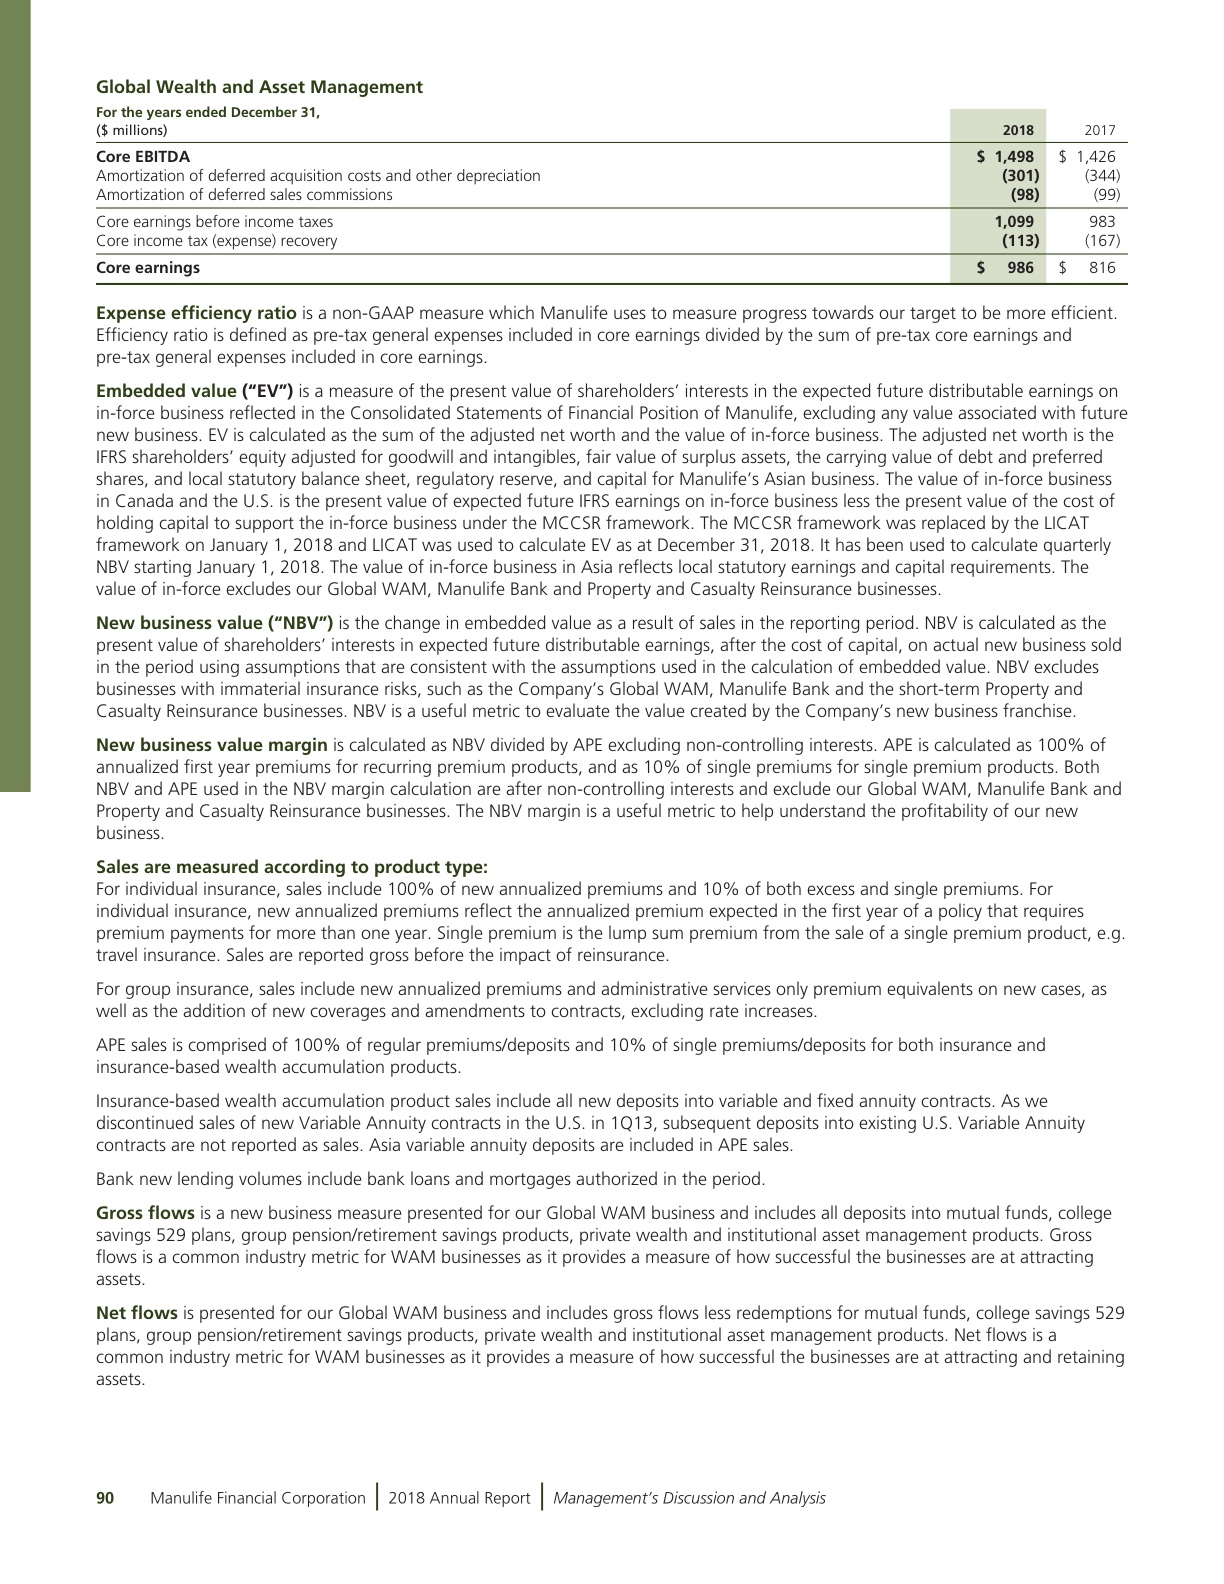
\includegraphics[width=0.8\textwidth]{test-resultaten/8/original.jpg}
    \caption{Origineel document.}
\end{figure}

\begin{figure}[H]
    \centering
    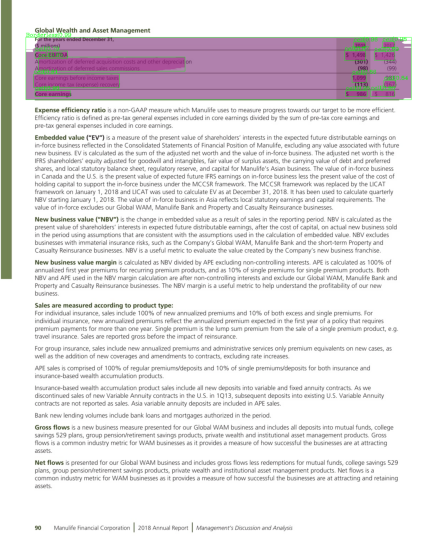
\includegraphics[width=0.8\textwidth]{test-resultaten/8/detected_tables.png}
    \caption{Gedetecteerde tabellen.}
\end{figure}

Getransformeerde tabellen met algoritme A:

\begin{tabular}{llll}
\toprule
{} &     For the years ended December 31,\textbackslash n(\$ millions) &          2018 &        2017 \\
\midrule
0 &  mortization of deferred acquisition costs and ... &       \$ 1,498 &     \$ 1,426 \\
1 &  Core earnings before income taxes\textbackslash nCore income... &  1,099\textbackslash n(113) &  983\textbackslash n(167) \\
2 &                                      Core earnings &        S\$ 986 &       \$ 816 \\
\bottomrule
\end{tabular}

Getransformeerde tabellen met algoritme B:

\begin{tabular}{lllll}
\toprule
{} &                   For the years ended December 31, &     NaN &           NaN &      NaN \\
\midrule
0 &                                       (§ millions) &    2018 &          None &     2017 \\
1 &                                        Core EBITDA &  \$1,498 &          None &  \$ 1,426 \\
2 &  Amortization of deferred acquisition costs and... &   (301) &  depreciation &    (344) \\
3 &         Amortization of deferred sales commissions &    (9a) &          None &     (99) \\
4 &                  Core earnings before income taxes &   1,099 &          None &      983 \\
5 &                        Core tax (expense) recovery &   (113) &          None &    (167) \\
6 &                                      Core earnings &   \$ 986 &          None &    \$ 816 \\
\bottomrule
\end{tabular}
\section{Document 9}

\begin{figure}[H]
    \centering
    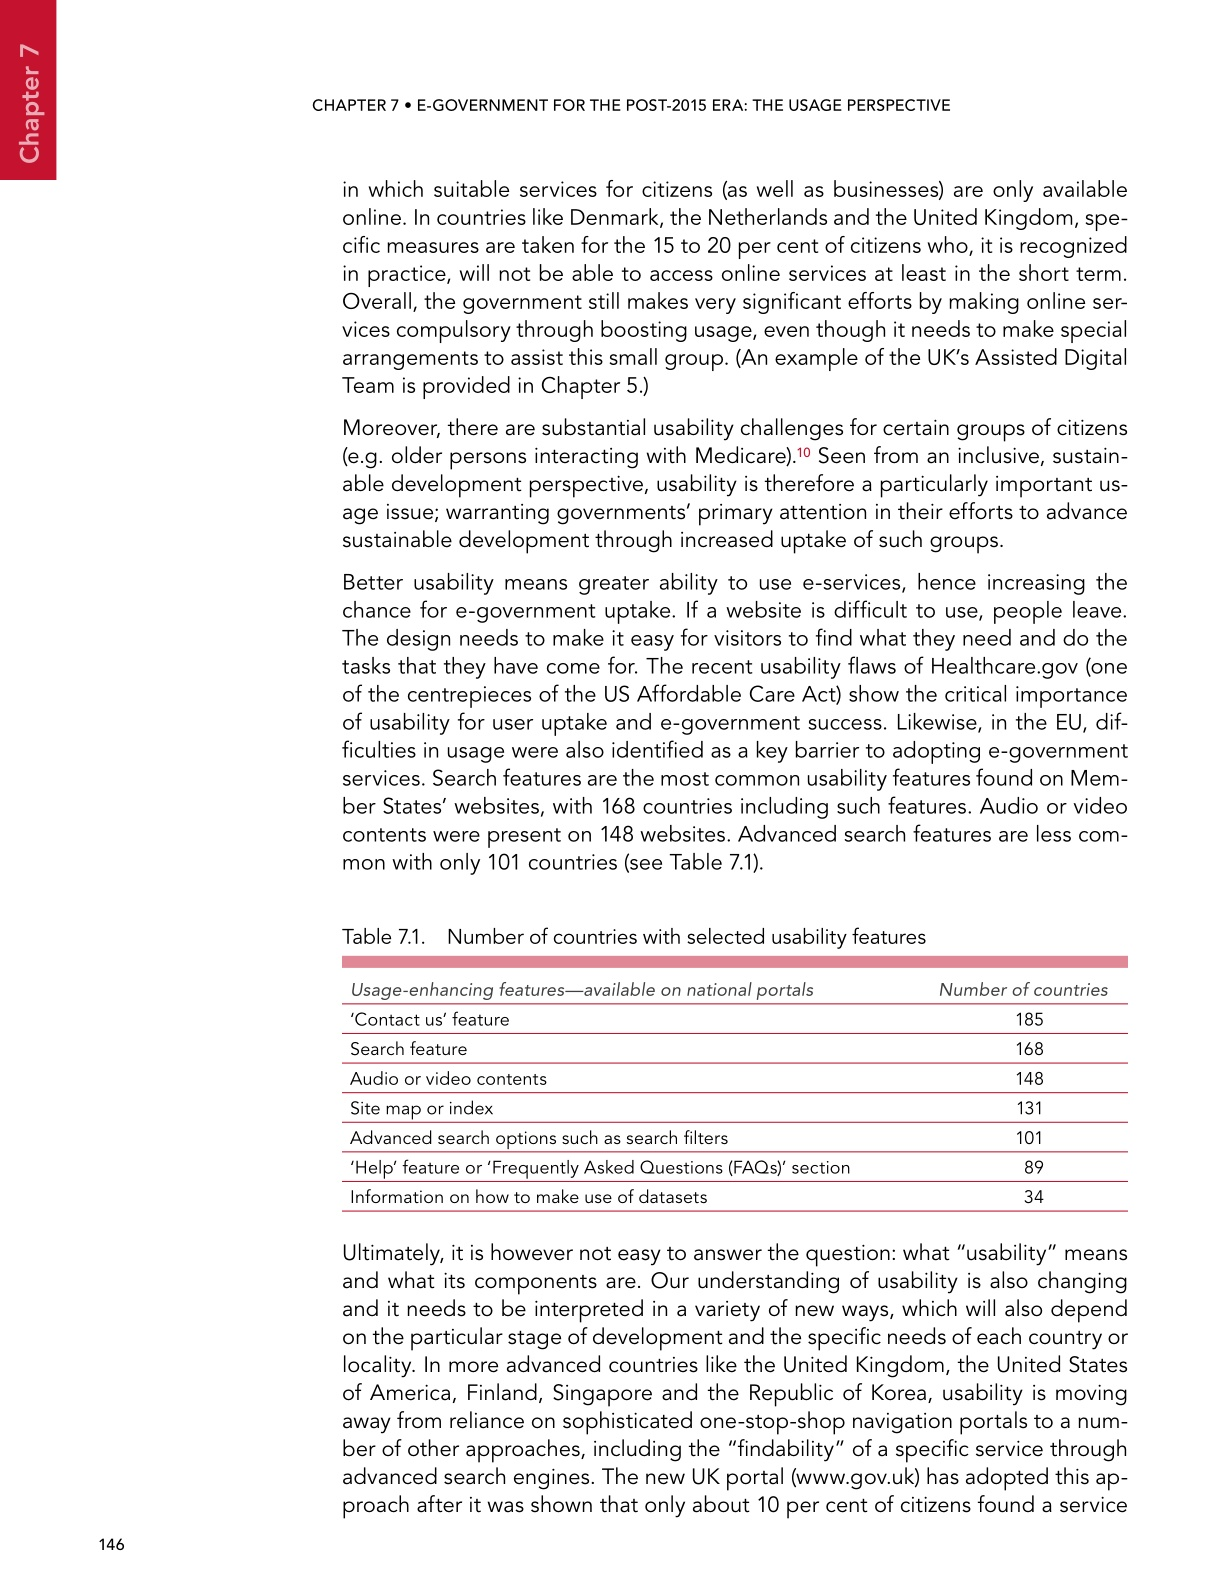
\includegraphics[width=0.8\textwidth]{test-resultaten/9/original.jpg}
    \caption{Origineel document.}
\end{figure}

\begin{figure}[H]
    \centering
    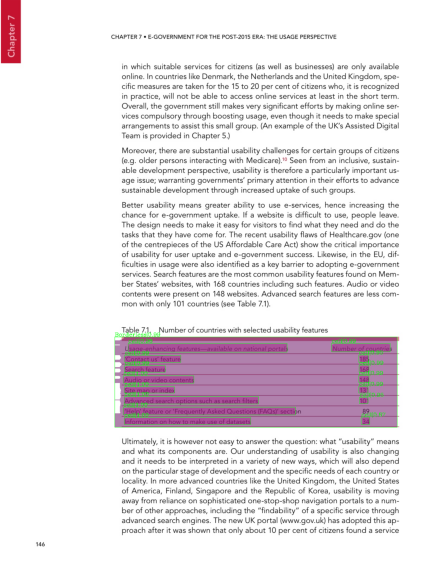
\includegraphics[width=0.8\textwidth]{test-resultaten/9/detected_tables.png}
    \caption{Gedetecteerde tabellen.}
\end{figure}

Getransformeerde tabellen met algoritme A:

\begin{tabular}{lll}
\toprule
{} & Usage-enhancing features—available on national portals & Number of countries \\
\midrule
0 &                               ‘Contact us’ feature &                 185 \\
1 &                                     Search feature &                 168 \\
2 &                            Audio or video contents &                 148 \\
3 &                                  Site map or index &                 131 \\
4 &     Advanced search options such as search filters &                 101 \\
5 &  ‘Help’ feature or ‘Frequently Asked Questions ... &                 B89 \\
6 &         Information on how to make use of datasets &                  34 \\
\bottomrule
\end{tabular}

Getransformeerde tabellen met algoritme B:

\begin{tabular}{lll}
\toprule
{} & Usage-enhancing features—available on national portals & Number of countries \\
\midrule
0 &                               ‘Contact us’ feature &                 185 \\
1 &                                     Search feature &                 168 \\
2 &                            Audio or video contents &                 148 \\
3 &                                  Site map or index &                 131 \\
4 &     Advanced search options such as search filters &                 101 \\
5 &  ‘Help’ feature or ‘Frequently Asked Questions ... &                  89 \\
6 &         Information on how to make use of datasets &                  34 \\
\bottomrule
\end{tabular}
\section{Document 10}

\begin{figure}[H]
    \centering
    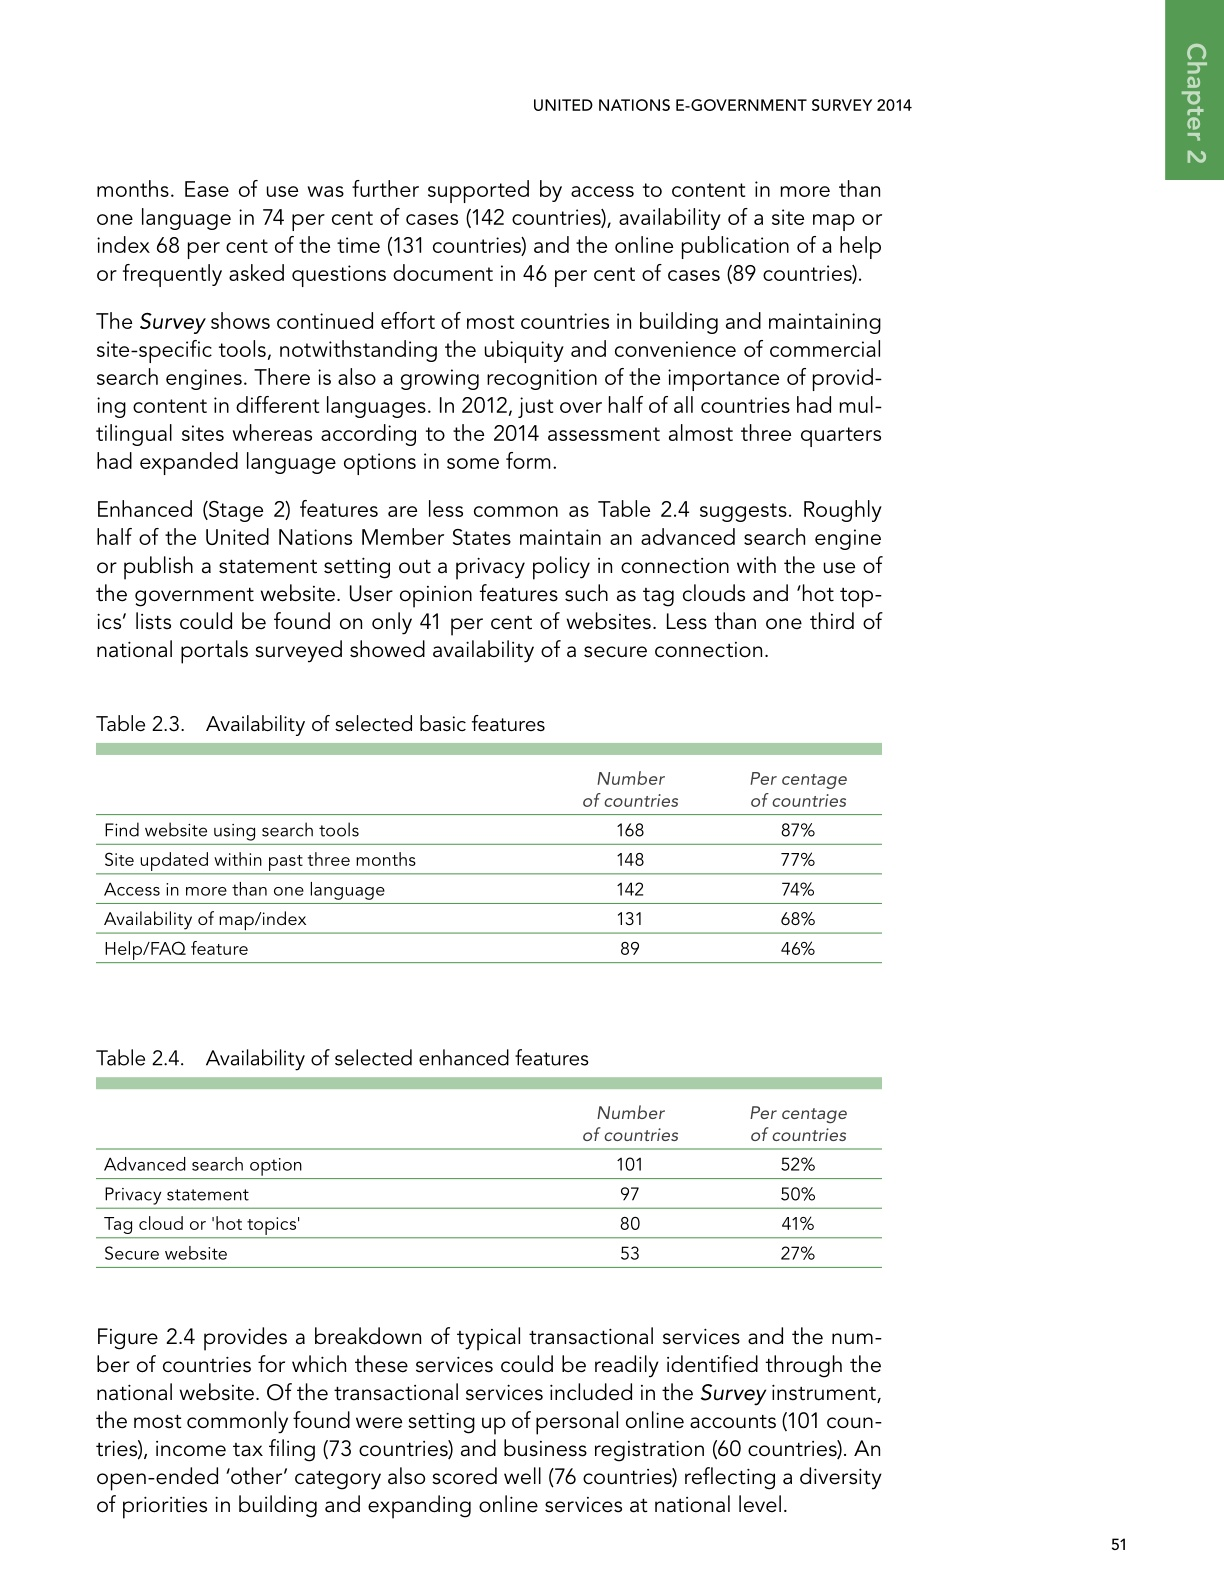
\includegraphics[width=0.8\textwidth]{test-resultaten/10/original.jpg}
    \caption{Origineel document.}
\end{figure}

\begin{figure}[H]
    \centering
    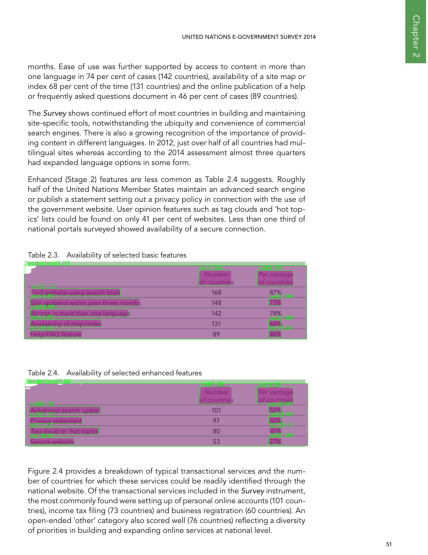
\includegraphics[width=0.8\textwidth]{test-resultaten/10/detected_tables.png}
    \caption{Gedetecteerde tabellen.}
\end{figure}

Getransformeerde tabellen met algoritme A:

\begin{tabular}{lll}
\toprule
{} &      Number\textbackslash nof countries & Per centage\textbackslash nof countries \\
\midrule
0 &    Advanced search optior &                       52\% \\
1 &         Privacy statement &                       50\% \\
2 &  Taq cloud or ‘hot topics &                       AIM \\
3 &            Secure website &                       27\% \\
\bottomrule
\end{tabular}

\begin{tabular}{lll}
\toprule
{} &                   Number\textbackslash nof countries & Per centage\textbackslash nof countries \\
\midrule
0 &        Find website using search tools &                       87\% \\
1 &  Site updated within past three months &                       77\% \\
2 &       Access in more than one lanquaas &                       TA\% \\
3 &              Availability of map/inde> &                       68\% \\
4 &                       Help/FAQ feature &                       Ab\% \\
\bottomrule
\end{tabular}

Getransformeerde tabellen met algoritme B:

\begin{tabular}{llll}
\toprule
{} &        Number &   Per centage &                        NaN \\
\midrule
0 &  of countries &  of countries &                       None \\
1 &           101 &           52\% &     Advanced search option \\
2 &            97 &           50\% &          Privacy statement \\
3 &            80 &           41\% &  Tag cloud or ‘hot topics’ \\
4 &            53 &           27\% &             Secure website \\
\bottomrule
\end{tabular}

\begin{tabular}{llll}
\toprule
{} &        Number &   Per centage &                                    NaN \\
\midrule
0 &  of countries &  of countries &                                   None \\
1 &           168 &           87\% &        Find website using search tools \\
2 &           148 &           71\% &  Site updated within past three months \\
3 &           142 &           74\% &       Access in more than one language \\
4 &           131 &           68\% &              Availability of map/index \\
5 &            89 &           46\% &                       Help/FAQ feature \\
\bottomrule
\end{tabular}
\section{Document 11}

\begin{figure}[H]
    \centering
    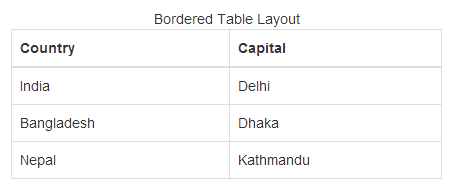
\includegraphics[width=0.8\textwidth]{test-resultaten/11/original.png}
    \caption{Origineel document.}
\end{figure}

\begin{figure}[H]
    \centering
    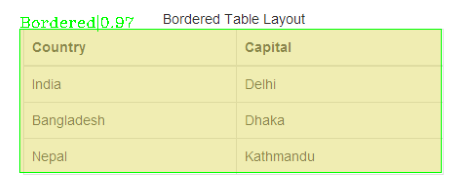
\includegraphics[width=0.8\textwidth]{test-resultaten/11/detected_tables.png}
    \caption{Gedetecteerde tabellen.}
\end{figure}

Getransformeerde tabellen met algoritme A:

\begin{tabular}{lll}
\toprule
{} &     Country &    Capital \\
\midrule
0 &       India &      Delhi \\
1 &  Bangladesh &      Dhaka \\
2 &       Nepal &  Kathmandu \\
\bottomrule
\end{tabular}

Getransformeerde tabellen met algoritme B:

\begin{tabular}{lll}
\toprule
{} &     Country &    Capital \\
\midrule
0 &       India &      Delhi \\
1 &  Bangladesh &      Dhaka \\
2 &       Nepal &  Kathmandu \\
\bottomrule
\end{tabular}
\section{Document 12}

\begin{figure}[H]
    \centering
    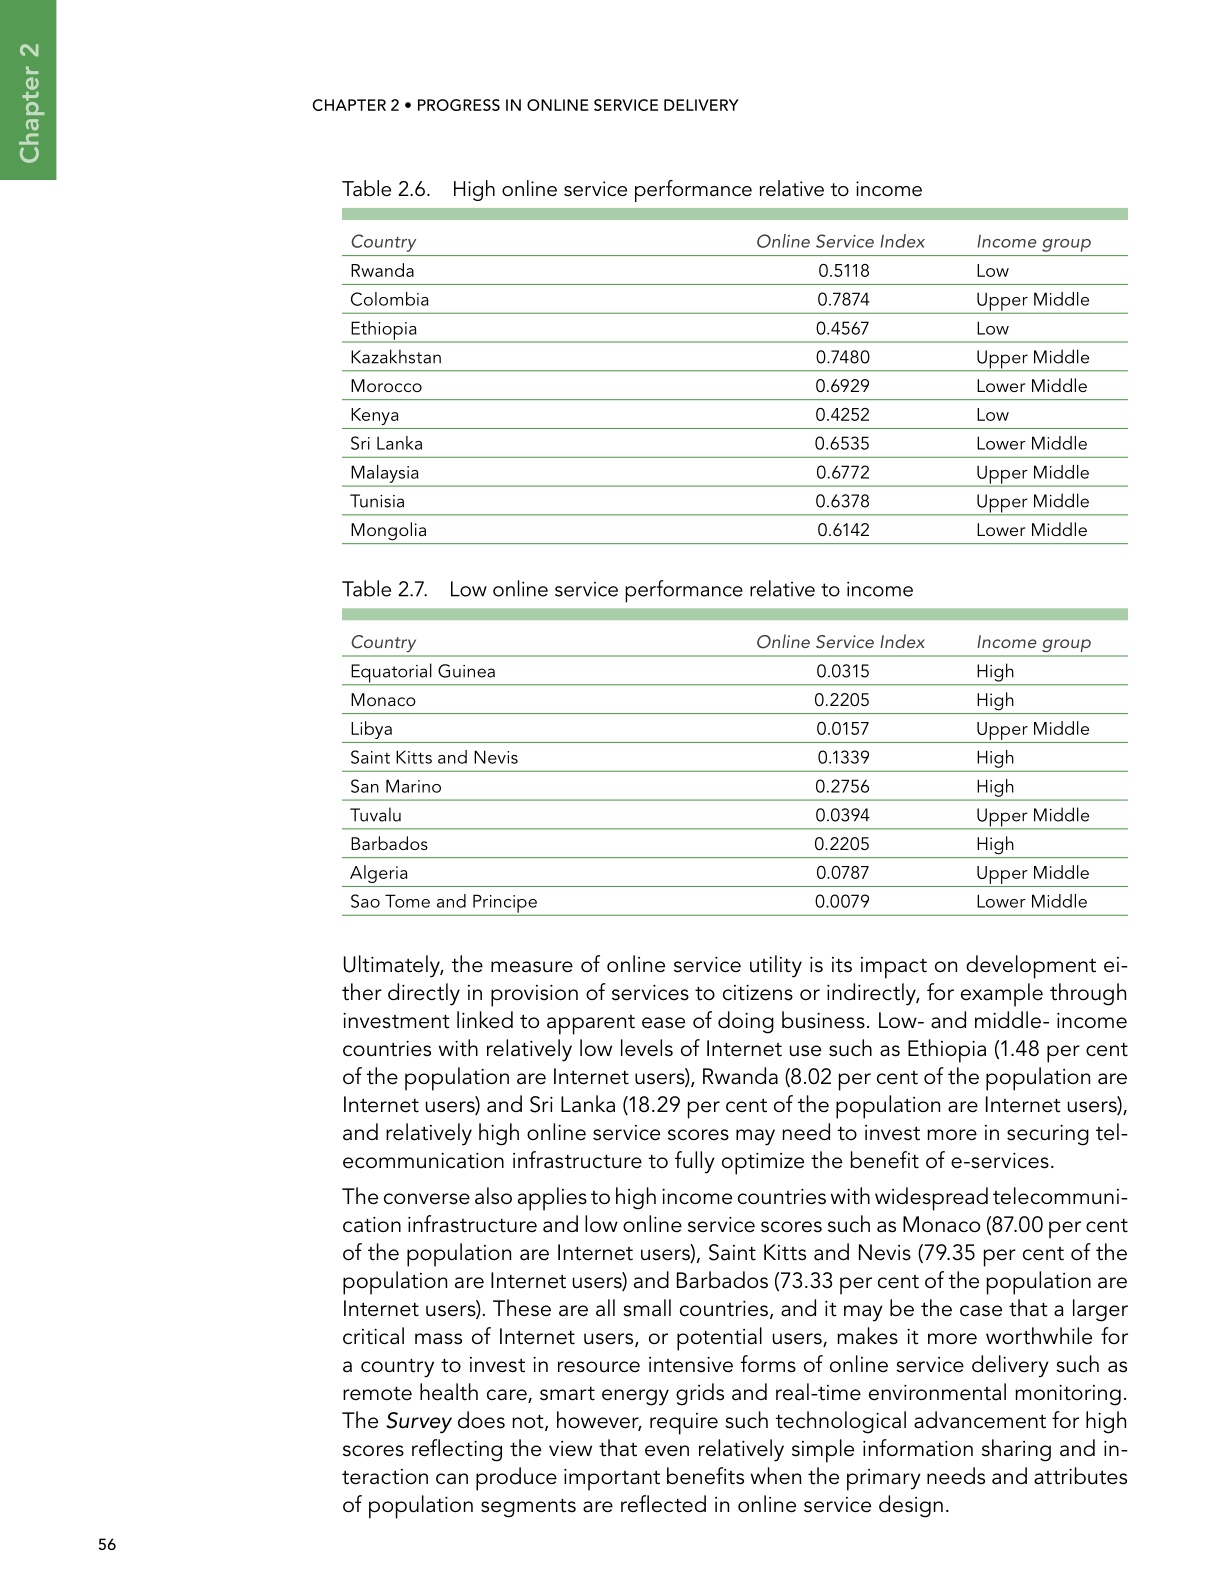
\includegraphics[width=0.8\textwidth]{test-resultaten/12/original.png}
    \caption{Origineel document.}
\end{figure}

\begin{figure}[H]
    \centering
    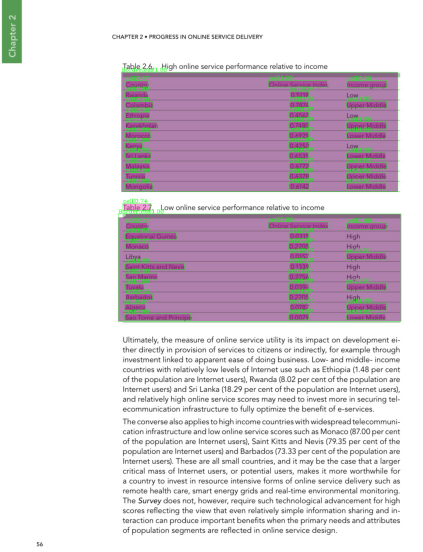
\includegraphics[width=0.8\textwidth]{test-resultaten/12/detected_tables.png}
    \caption{Gedetecteerde tabellen.}
\end{figure}

Getransformeerde tabellen met algoritme A:

\begin{tabular}{llll}
\toprule
{} &                Country & Online Service Index &  Income group \\
\midrule
0 &      Equatorial Guinez &               0.0315 &          High \\
1 &                 Monaco &               0.2205 &          None \\
2 &                  Libya &               0.0157 &  Upper Middle \\
3 &  Saint Kitts and Nevis &               0.1339 &          High \\
4 &             San Marino &               0.2756 &          High \\
5 &                 Tuvalu &               0.0394 &  Upper Middle \\
6 &               Barbados &               0.2205 &          None \\
7 &                Algeria &               0.0787 &  Upper Middle \\
8 &  Sao Tome and Principe &               0.0079 &  Lower Middle \\
\bottomrule
\end{tabular}

\begin{tabular}{llll}
\toprule
{} &     Country & Online Service Index &  Income group \\
\midrule
0 &      Rwanda &               0.5118 &           Low \\
1 &    Colombia &               0.7874 &  Upper Middle \\
2 &    Ethiopia &               0.4567 &           Low \\
3 &  Kazakhstan &               0.7480 &  Upper Middle \\
4 &     Morocco &               0.6929 &  Lower Middle \\
5 &       Kenya &               0.4252 &           Low \\
6 &   Sri Lanka &               0.6535 &  Lower Middle \\
7 &    Malaysia &               0.6772 &  Upper Middle \\
8 &     Tunisia &               0.6378 &  Upver Middle \\
9 &    Mongolia &               0.6142 &  Lower Middle \\
\bottomrule
\end{tabular}

Getransformeerde tabellen met algoritme B:

\begin{tabular}{llll}
\toprule
{} &                Country & Online Service Index &  income group \\
\midrule
0 &      Equatorial Guinea &               0.0315 &          High \\
1 &                 Monaco &               0.2205 &          High \\
2 &                  Libya &               0.0157 &  Upper Middle \\
3 &  Saint Kitts and Nevis &               0.1339 &          High \\
4 &             San Marino &               0.2756 &          High \\
5 &                 Tuvalu &               0.0394 &  Upper Middle \\
6 &               Barbados &               0.2205 &          High \\
7 &                Algeria &               0.0787 &  Upper Middle \\
8 &  Sao Tome and Principe &               0.0079 &  Lower Middle \\
\bottomrule
\end{tabular}

\begin{tabular}{llll}
\toprule
{} &     Country & Online Service index & \_\_Income group \\
\midrule
0 &      Rwanda &               0.5118 &            Low \\
1 &    Colombia &               0.7874 &   Upper Middle \\
2 &    Ethiopia &               0.4567 &            Low \\
3 &  Kazakhstan &               0.7480 &   Upper Middle \\
4 &    Morocco. &               0.6929 &   Lower Middle \\
5 &       Kenya &               0.4252 &            Low \\
6 &   Sti Lanka &               0.6535 &   Lower Middle \\
7 &    Malaysia &               0.6772 &   Upper Middle \\
8 &     Tunisia &               0.6378 &   Upper Middle \\
9 &    Mongolia &               0.6142 &   Lower Middle \\
\bottomrule
\end{tabular}

\section{Document 13}

\begin{figure}[H]
    \centering
    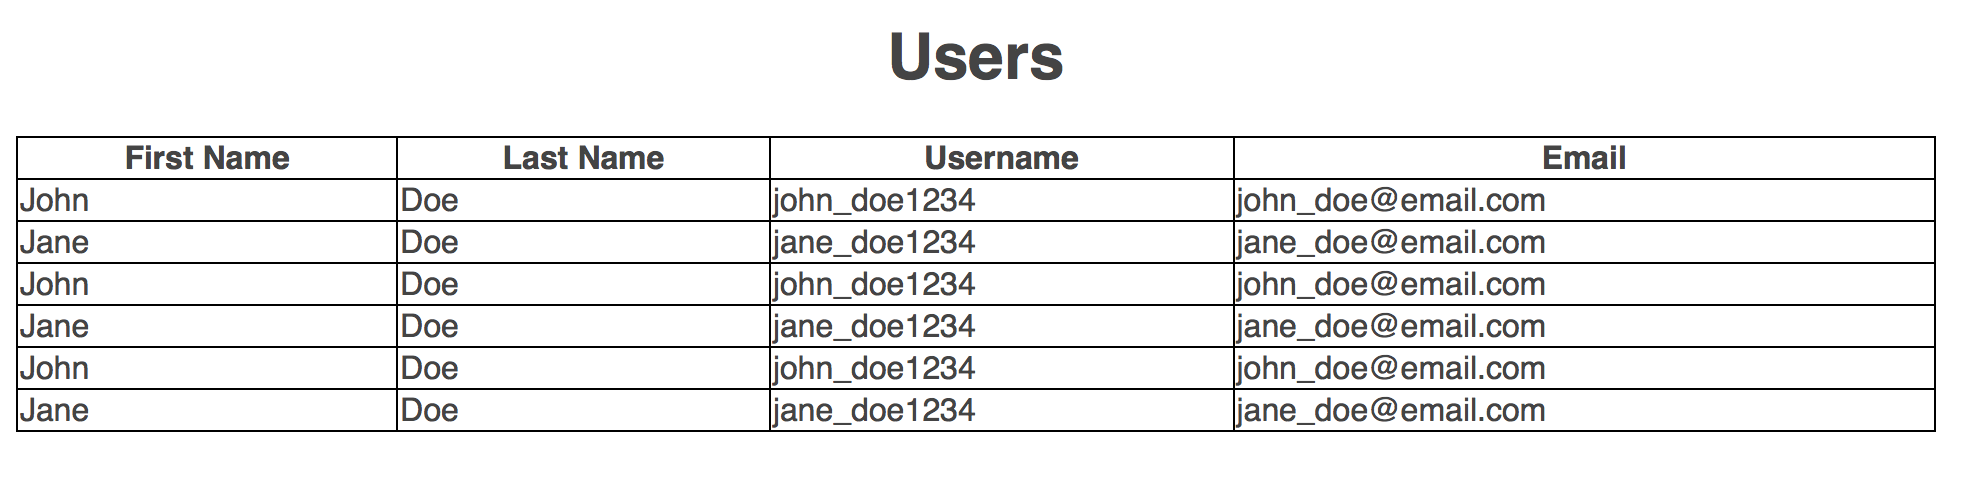
\includegraphics[width=0.8\textwidth]{test-resultaten/13/original.png}
    \caption{Origineel document.}
\end{figure}

\begin{figure}[H]
    \centering
    \includegraphics[width=0.8\textwidth]{test-resultaten/13/detected_tables.png}
    \caption{Gedetecteerde tabellen.}
\end{figure}

Getransformeerde tabellen met algoritme A:

Tabeltransformatie gefaald.

Getransformeerde tabellen met algoritme B:

\begin{tabular}{lllll}
\toprule
{} & First Name & Last Name &       Username &                Email \\
\midrule
0 &       John &       Doe &   john\_doe1234 &   john\_doe@email.com \\
1 &       Jane &       Doe &   jane\_doe1234 &   jane\_doe@email.com \\
2 &       John &       Doe &   john\_doe1234 &   john\_doe@email.com \\
3 &       Jane &       Doe &   jane\_doe1234 &   jane\_doe@email.com \\
4 &       John &       Doe &   john\_doe1234 &   john\_doe@email.com \\
5 &       Jane &       Doe &  \textbackslash jane\_doe1234 &  \textbackslash jane\_doe@email.com \\
\bottomrule
\end{tabular}

\section{Document 14}

\begin{figure}[H]
    \centering
    \includegraphics[width=0.8\textwidth]{test-resultaten/14/original_b/original.png}
    \caption{Origineel document.}
\end{figure}

\begin{figure}[H]
    \centering
    \includegraphics[width=0.8\textwidth]{test-resultaten/14/original_b/detected_tables.png}
    \caption{Gedetecteerde tabellen.}
\end{figure}

Getransformeerde tabellen met algoritme A:

Tabeltransformatie gefaald.

Getransformeerde tabellen met algoritme B:

\begin{tabular}{llllll}
\toprule
{} &   Average aty &   per & serving &    NaN &  100mL \\
\midrule
0 &        Energy &  None &   775kd &   None &  310kJ \\
1 &       Protein &  None &    9.09 &   None &   3.69 \\
2 &    Fat -Total &  None &   10.3g &   None &    41g \\
3 &   - Saturated &  None &    6.0g &   None &   2.49 \\
4 &  Carbohydrate &  None &   11.89 &   None &    4/9 \\
5 &      - Sugars &  None &   11.89 &   None &    479 \\
6 &        sodium &  None &    None &   None &   None \\
7 &          None &  None &   145mg &   None &   58mg \\
8 &       Calcium &  (38\% &   RDI*) &  308mg &  123mg \\
\bottomrule
\end{tabular}
\section{Document 15}

\begin{figure}[H]
    \centering
    \includegraphics[width=0.8\textwidth]{test-resultaten/15/orignal.png}
    \caption{Origineel document.}
\end{figure}

\begin{figure}[H]
    \centering
    \includegraphics[width=0.8\textwidth]{test-resultaten/1/detected_tables.png}
    \caption{Gedetecteerde tabellen.}
\end{figure}

Getransformeerde tabellen met algoritme A:

\begin{tabular}{llll}
\toprule
{} &                                Opleidingsprogramma &         WE & 12 Creditbewi\textbackslash n15 Creditbewljs\textbackslash n12 Creditbewijs\textbackslash n16 Creditbewijs \\
\midrule
0 &               2 Bedrijfsmanagement\textbackslash n3. Analyse Ill &   3 EK1/S1 &                   12 Creditbewijs\textbackslash n15 Creditbewijs \\
1 &  3 Internationale Communicatie III\textbackslash n3. Artifici... &   3 EK1/S1 &                   12 Creditbewijs\textbackslash n16 Creditbewijs \\
2 &            Native apps |: mobile apps voor Android &   3 EK1/S1 &                                   Afwezig - Tweede \\
3 &      3 .\textasciitilde =Native apps II: mobile apps voor Windows &   4 EK1/S1 &                                   Afwezig - Tweede \\
4 &                                           Web apps &   3 FK1IS1 &                                   Afwezig - Tweede \\
5 &                     3 \textasciitilde \textasciitilde  \textasciitilde Project Ill: Mobile apps &   5 EK1/S1 &                                    15 Creditbewijs \\
6 &                                             Talent &   3 EK1IS2 &                                    15 Creditbewijs \\
7 &  Internationale stage S2 20STP\textbackslash nBachelorproef S... &  20 EK1/S2 &                                               None \\
8 &                          3  =Bachelorproef SJ 7STP &   7 EK1IS2 &                      Afwezig - Tweede\textbackslash n‘examenkans \\
\bottomrule
\end{tabular}

Getransformeerde tabellen met algoritme B:

\begin{tabular}{llll}
\toprule
{} &                          Opleidingsprogramma &    ‘SP Examen &  Seore Opmerking \\
\midrule
0  &                         2 Bedrijfsmanagement &      3 EK1|S1 &      Creditbewjs \\
1  &                                3 Analyse Ill &      3 EK1|S1 &      Creditbewjs \\
2  &            3 Internationale Communicatie Ill &      3 EK1|S1 &      Creditbewjs \\
3  &                  3 Artificiéle Intelligentie &      3 EK1|S1 &      Creditbewjs \\
4  &   3. Native apps |: mobile apps voor Android &      3 EK1|S1 &  Afwezig- Tweede \\
5  &  3. Native apps Il: mobile apps voor Windows &      4 EK1|S1 &  Afwezig- Tweede \\
6  &                                  3. Web apps &      3 EK1|S1 &  Afwezig- Tweede \\
7  &                   3 Project Ill: Mobile apps &      \$ EK1|S1 &   15 Creditbewjs \\
8  &                                    3 iTalent &      3 EK1|S2 &   15 Creditbewjs \\
9  &              3 Internationale stage \$2 20STP &  20 20 EK1|S2 &      7 Verworven \\
10 &                      3 Bachelorproef SJ 7STP &           7 7 &  Afwezig- Tweede \\
11 &                                         None &          None &       examenkans \\
12 &                                         None &          None &       examenkans \\
13 &                                         None &          None &       examenkans \\
\bottomrule
\end{tabular}
\section{Document 16}

\begin{figure}[H]
    \centering
    \includegraphics[width=0.8\textwidth]{test-resultaten/16/original.png}
    \caption{Origineel document.}
\end{figure}

\begin{figure}[H]
    \centering
    \includegraphics[width=0.8\textwidth]{test-resultaten/16/detected_tables.png}
    \caption{Gedetecteerde tabellen.}
\end{figure}

Getransformeerde tabellen met algoritme A:

\begin{tabular}{lllllll}
\toprule
{} & Seizoen &                                  Locatie &     Rol leerkrachi &       Statuut &                 Status &  Download \\
\midrule
0 &   2018s &  Hogeschool Gent - Campus\textbackslash nSchoonmeersen &  Series\textbackslash nAssistant &  Vrijwilliger &  Contract is in\textbackslash ncorde &        as \\
1 &   2018w &                     GO! Middenschool MAD &  Series\textbackslash nAssistant &    Jobstudent &  Contract is in\textbackslash ncorde &  Download \\
2 &   2018w &  Hogeschool Gent - Campus\textbackslash nSchoonmeersen &  Series\textbackslash nAssistant &    Jobstudent &  Contract is in\textbackslash ncorde &        as \\
3 &   2019s &                     GO! Middenschool MAD &  Series\textbackslash nAssistant &    Jobstudent &  Contract is in\textbackslash ncorde &  Download \\
4 &   2019s &  Hogeschool Gent - Campus\textbackslash nSchoonmeersen &  Series\textbackslash nAssistant &    Jobstudent &  Contract is in\textbackslash ncorde &        as \\
5 &   2019W &  Hogeschool Gent - Campus\textbackslash nSchoonmeersen &  Series\textbackslash nAssistant &    Jobstudent &  Contract is in\textbackslash ncorde &        as \\
\bottomrule
\end{tabular}


Getransformeerde tabellen met algoritme B:

\begin{tabular}{lllllll}
\toprule
{} & Seizoen &                                 Locatie &    Rol leerkracht &       Statuut &                Status &  Download \\
\midrule
0 &   20188 &  Hogeschool Gent - Campus Schoonmeersen &  Series Assistant &  Vrijwilliger &  Contract is in corde &  Download \\
1 &   20180 &                    GO! Middenschool MAD &  Series Assistant &    dobstudent &  Contract is in corde &  Download \\
2 &   20180 &  Hogeschool Gent - Campus Schoonmeersen &  Series Assistant &    dobstudent &  Contract is in corde &  Download \\
3 &   20198 &                    GO! Middenschool MAD &  Series Assistant &    dobstudent &  Contract is in corde &  Download \\
4 &   20198 &  Hogeschool Gent - Campus Schoonmeersen &  Series Assistant &    dobstudent &  Contract is in corde &  Download \\
5 &   2019" &  Hogeschool Gent - Campus Schoonmeersen &  Series Assistant &    dobstudent &   Contract is in orde &  Download \\
\bottomrule
\end{tabular}
\section{Document 17}

\begin{figure}[H]
    \centering
    \includegraphics[width=0.8\textwidth]{test-resultaten/17/original.png}
    \caption{Origineel document.}
\end{figure}

\begin{figure}[H]
    \centering
    \includegraphics[width=0.8\textwidth]{test-resultaten/17/detected_tables.png}
    \caption{Gedetecteerde tabellen.}
\end{figure}

Getransformeerde tabellen met algoritme A:

\begin{tabular}{lllll}
\toprule
{} & S. No. &    Name &        City & Age \\
\midrule
0 &      1 &    Ajay &       Patna &  20 \\
1 &      2 &   Rahul &  Chandigarh &  17 \\
2 &      3 &  Parush &     Kolkata &  22 \\
\bottomrule
\end{tabular}

Getransformeerde tabellen met algoritme B:

\begin{tabular}{lllll}
\toprule
{} & S.No. &    Name &        City & Age \\
\midrule
0 &     1 &    Ajay &       Patna &  20 \\
1 &     2 &   Rahul &  Chandigarh &   7 \\
2 &     3 &  Parush &     Kolkata &  22 \\
\bottomrule
\end{tabular}
\section{Document 18}

\begin{figure}[H]
    \centering
    \includegraphics[width=0.8\textwidth]{test-resultaten/18/original.png}
    \caption{Origineel document.}
\end{figure}

\begin{figure}[H]
    \centering
    \includegraphics[width=0.8\textwidth]{test-resultaten/18/detected_tables.png}
    \caption{Gedetecteerde tabellen.}
\end{figure}

Getransformeerde tabellen met algoritme A:

\begin{tabular}{lllll}
\toprule
{} & No\textbackslash nresponse & No surveys\textbackslash nknown & Total of\textbackslash nType & Surveys:\textbackslash nidentified \\
\midrule
0 &            4 &                 8 &             14 &                 None \\
1 &           11 &                 8 &             22 &                    3 \\
2 &            1 &                 3 &              4 &                 None \\
3 &            4 &                 4 &           None &                 None \\
4 &            2 &                 6 &              8 &                    2 \\
5 &            2 &                 5 &              7 &                 None \\
6 &            2 &                 6 &              9 &                   41 \\
7 &            2 &                 3 &           None &                 None \\
8 &            2 &                 4 &              2 &                 None \\
9 &            2 &                 5 &              6 &                 None \\
\bottomrule
\end{tabular}


Getransformeerde tabellen met algoritme B:

\begin{tabular}{llllll}
\toprule
{} &              Type of Organisation & No response & Nosurveys | known & | Totalof Type & | Surveys identified \\
\midrule
0  &             European Institutions &        None &                 2 &              3 &                    4 \\
1  &           Government / Regulators &          “4 &                 a &              4 &                    2 \\
2  &  Ait Navigation Service Providers &          14 &                 a &              2 &                    3 \\
3  &               Airport Authorities &           4 &                 3 &              4 &                 None \\
4  &                           Airines &           4 &              None &              4 &                 None \\
5  &      Representative Organisations &           2 &                 6 &              a &                    2 \\
6  &       Pressure Groups / Watchdogs &        None &                 2 &              4 &                    2 \\
7  &    Commercial Market Researchers, &        None &                 2 &              5 &                    6 \\
8  &             Research Laboratories &           2 &                 5 &              7 &                 None \\
9  &                          Academia &           2 &                 6 &              9 &                    4 \\
10 &                            TOTALS &          26 &                42 &             BD &                   20 \\
\bottomrule
\end{tabular}
\section{Document 19}

\begin{figure}[H]
    \centering
    \includegraphics[width=0.8\textwidth]{test-resultaten/19/original.png}
    \caption{Origineel document.}
\end{figure}

\begin{figure}[H]
    \centering
    \includegraphics[width=0.8\textwidth]{test-resultaten/19/detected_tables.png}
    \caption{Gedetecteerde tabellen.}
\end{figure}

Getransformeerde tabellen met algoritme A:

\begin{tabular}{lll}
\toprule
{} &      Brennwert & 234 kcal / 980 kJ \\
\midrule
0 &  Kohlenhydrate &              2,69 \\
1 &      Eiweif\&BQ &             15,89 \\
2 &           Fett &              28 9 \\
\bottomrule
\end{tabular}

Getransformeerde tabellen met algoritme B:

\begin{tabular}{llll}
\toprule
{} & Nahrwerte pro 100 9 & Flohsamen (Zirkulin) & Gemahlene Flohsamenschalen (dm) \\
\midrule
0 &           Brennwert &    234 keal / 980 kd &               208 keal / 842 kJ \\
1 &       Kohlenhydrate &                  264 &                              og \\
2 &              EiweiB &                15,84 &                             389 \\
3 &                Fett &                  289 &     2.8 g. davon gesattigt: 1.9 \\
4 &       Ballaststoffe &                  68g &                             Bag \\
\bottomrule
\end{tabular}
\section{Document 20}

\begin{figure}[H]
    \centering
    \includegraphics[width=0.8\textwidth]{test-resultaten/20/original.png}
    \caption{Origineel document.}
\end{figure}

\begin{figure}[H]
    \centering
    \includegraphics[width=0.8\textwidth]{test-resultaten/20/detected_tables.png}
    \caption{Gedetecteerde tabellen.}
\end{figure}

Getransformeerde tabellen met algoritme A:

Tabeltransformatie gefaald.

Getransformeerde tabellen met algoritme B:

\begin{tabular}{lllll}
\toprule
{} &                          Chronische medicatie &   Frequentie &           NaN &                                        Opmerkingen \\
\midrule
2 &    ASAFLOW 80MG MAAGSAPRES COMP BLI 168X 80MG &    Dagelijks &    04/09/2015 &  Indicatie: Bloedverdunner Instructie: Bij begi... \\
3 &                   AZILECT 1 MG TABL 28 X 1 MG &    Dagelijks &    04/09/2015 &                               Indicatie: Parkinson \\
4 &                   FORLAX PI PHARMA 20 ZAK 10G &  | Dagelijks &    04/09/2015 &  Indicatie: Stoelgang Instructie: Oplossen in glas \\
5 &                          INDERAL COMP 50X10MG &         None &    04/09/2015 &                         Indicatie: Beven/parkinson \\
6 &  MIRAPEXIN 3,15 MG COMP VERLENGDE AFGIFTE 100 &   | Dageliks &  | 04/09/2015 &                               Indicatie: Parkinson \\
7 &                   STALEVO 100/25/200 100 TABL &   | Dageliks &  | 04/09/2015 &                               Indicatie: Parkinson \\
\bottomrule
\end{tabular}
\section{Document 21}

\begin{figure}[H]
    \centering
    \includegraphics[width=0.8\textwidth]{test-resultaten/21/original.png}
    \caption{Origineel document.}
\end{figure}

\begin{figure}[H]
    \centering
    \includegraphics[width=0.8\textwidth]{test-resultaten/21/detected_tables.png}
    \caption{Gedetecteerde tabellen.}
\end{figure}

Getransformeerde tabellen met algoritme A:

Tabeltransformatie gefaald.

Getransformeerde tabellen met algoritme B:

\begin{tabular}{llllll}
\toprule
{} &                           ineotions &     8h &   ith &       | &  | oo \\
\midrule
1  &                  MEDICAMENTS Per Os &   None &  None &    None &  None \\
2  &                    PAROXETINE 20 mg &      1 &  None &    None &  None \\
3  &                         FOLAVIT 4mg &      1 &  None &    None &  None \\
4  &                   ALDACTONE cp 25mg &      = &  None &    None &  None \\
5  &            ALLOPURINOL SANDOZ 100mg &   None &  None &       4 &  None \\
6  &                  BURINEX LEO cp 5mg &   None &  None &    None &  None \\
7  &                      CEREVISIA caps &   None &  None &    None &  None \\
8  &                   GLURENORM cp 30mg &   None &  None &    None &  None \\
9  &  L THYROXINE CHRISTIAENS cp0,025 mg &   None &  None &    None &  None \\
10 &     L THYROXINE CHRISTIAENS cp0,1mg &   None &  None &    None &  None \\
11 &               LERCANIDIPINE EG 10mg &     3] &  None &    None &  None \\
12 &                 MOXONIDINE EG 0,4mg &   None &  None &    None &    41 \\
13 &                  PARACETAMOL EG 1gr &      1 &    41 &      41 &  None \\
14 &                    LORMETAZEPAM 2mg &   None &  None &    None &   112 \\
15 &                         PROLOPA 250 &     4a &  None &    None &    14 \\
16 &                      SELECTOL 400mg &     12 &  None &    None &    12 \\
17 &                           SPASMOMEN &     41 &  None &    None &    41 \\
18 &               TEMESTA EXPIDET 2,5mg &   None &  None &    None &    41 \\
19 &                        VIPIDIA 25mg &    412 &  None &    None &  None \\
20 &                      URI-CRAN FORTE &     41 &  None &    None &  None \\
21 &                      CALCIUM en Gel &   None &  None &      41 &  None \\
22 &              D CURE 1x/sem le jeudi &   None &  None &    None &  None \\
23 &                      MOVICOL SACHET &      1 &  None &    None &  None \\
25 &                       TRADONAL ODIS &     41 &  None &    None &  None \\
26 &                         MOTILIUM SN &   None &  None &    None &  None \\
27 &               PLACEBO (pour dormir) &   None &  None &    None &     4 \\
28 &          DIVERS (sirop, collyre...) &   None &  None &    None &  None \\
29 &                       GAVISCON ANIS &  410ml &     | &  | 10m1 &  None \\
\bottomrule
\end{tabular}
\section{Document 22}

\begin{figure}[H]
    \centering
    \includegraphics[width=0.8\textwidth]{test-resultaten/22/original.png}
    \caption{Origineel document.}
\end{figure}

\begin{figure}[H]
    \centering
    \includegraphics[width=0.8\textwidth]{test-resultaten/22/detected_tables.png}
    \caption{Gedetecteerde tabellen.}
\end{figure}

Getransformeerde tabellen met algoritme A:

Tabeltransformatie gefaald.

Getransformeerde tabellen met algoritme B:

\begin{tabular}{llllllllll}
\toprule
{} & Jaarlijkse gro) «| &             Naam =e & | 2 | 1990 &         2000 &    Inw. 2006 &  Inw. | 2013 & Opperviakte | | in km™ & sum? « &      Deelstaat | erste keer \\
\midrule
0  &               1,38 &             Berlijn &  3.433.695 &  | 3.382.169 &  | 3.404.037 &  | 3.421.829 &                 891,70 &  3.837 &              1749 | Berliin \\
1  &               0,70 &             Hamburg &  1.652.363 &  | 1.715.392 &  | 1.754.182 &  | 1.746.342 &                 755,30 &   2312 &              1787 | Hamburg \\
2  &               1,41 &            Miinchen &  1,229,026 &  | 1.210.223 &  | 1.294.608 &  | 1.407.836 &                 310,70 &  4.531 &              1854 | Beieren \\
3  &               0,96 &              Keulen &   953.551] &     962.884] &     989.766] &    1.034.175 &                 405,16 &  2.553 &  1855 | Noordrijn-Westfalen \\
4  &               1,97 &  Frankfurt am Main| &   644.865] &      648.550 &     652.610] &      701.350 &                 248,31 &   2824 &               1875 | Hessen \\
5  &               1,06 &           Stuttgart &       None &     583.874] &     593.923] &      604.297 &                 207,35 &   2914 &   1874 | Baden-Wiirttemberg \\
6  &               0,84 &          Dusseldorf &       None &     569.364] &     577.505) &      598.686 &                 217,41 &   2754 &  1882 | Noordrijn-Westfalen \\
7  &               0,67 &            Dortmund &   599.055] &     588.994] &     587.624) &      575.944 &                 280,71 &  2.052 &  1895 | Noordrijn-Westfalen \\
8  &               0,53 &               Essen &   626.973] &     595.243] &     583.198] &      569.884 &                 210,30 &  2.710 &  1896 | Noordrijn-Westfalen \\
9  &               0,38 &              Bremen &   551.219] &     539.403] &     547.934) &      548.547 &                 325,42 &  1.686 &               1875 | Bremen \\
10 &               2,06 &             Leipzig &   511,079] &     493.208] &     506.578) &      531.562 &                 297,37 &  1.788 &               1871 | Saksen \\
11 &               1,08 &             Dresden &   490.571] &     477.807| &     504.795] &      530.754 &                 328,31 &  1.617 &               1852 | Saksen \\
12 &               0,83 &            Hannover &   513.010| &     515.001] &     516.343) &      518.386 &                 204,14 &  2.539 &          1873 | Nedersaksen \\
13 &               0,76 &          Neurenberg &    493,692 &     488.400] &     500.855) &      498.876 &                 186,37 &  2.677 &              1881 | Beieren \\
14 &               0,01 &            Duisburg &       None &     514.915| &     499.111] &     486.855. &                 232,80 &  2.091 &   1904. Noordrijn-Westfalen \\
\bottomrule
\end{tabular}
\section{Document 23}

\begin{figure}[H]
    \centering
    \includegraphics[width=0.8\textwidth]{test-resultaten/23/original.png}
    \caption{Origineel document.}
\end{figure}

\begin{figure}[H]
    \centering
    \includegraphics[width=0.8\textwidth]{test-resultaten/23/detected_tables.png}
    \caption{Gedetecteerde tabellen.}
\end{figure}

Getransformeerde tabellen met algoritme A:

\begin{tabular}{llll}
\toprule
{} &          Type &                                               Item &             Price \\
\midrule
0 &           CPU &   AMD Ryzen 5 1600 (12nm) 3.2 GHz 6-Core Processor &  \$104.99 @ Amazon \\
1 &   Motherboard &     “Gigabyte B450M DS3H Micro ATX AM4 Motherboard &      \$77.99 @ B\&H \\
2 &        Memory &  “Corsair Vengeance LPX 16 GB (2 x 8 GB) DDR4-3... &   \$30.55 @ Amazon \\
3 &       Storage &  *Team T-Force VULCAN 500 GB 2.5" Solid State D... &   \$55.99 @ Amazon \\
4 &    Video Card &   *EVGA GeForce RTX 2060 6 GB KO GAMING Video Card &  \$303.98 @ Newegg \\
5 &          Case &                   “Cougar MX330 ATX Mid Tower Case &      \$49.99 @ B\&H \\
6 &  Power Supply &                                    \$53 06 @ Amazo! &              None \\
7 &         Total &                                            \$676.55 &              None \\
\bottomrule
\end{tabular}

Getransformeerde tabellen met algoritme B:

\begin{tabular}{llll}
\toprule
{} &          Type &                                               Item &             Price \\
\midrule
0 &           cPU &   AMD Ryzen 5 1600 (12nm) 3.2 GHz 6-Core Processor &  \$104.99 @ Amazon \\
1 &   Motherboard &     *Gigabyte B450M DS3H Micro ATX AM4 Motherboard &      \$77.99 @ B\&H \\
2 &        Memory &  “Corsair Vengeance LPX 16 GB (2 x 8 GB) DDR4-3... &   \$30.55 @ Amazon \\
3 &       Storage &  “Team T-Force VULCAN 500 GB 2.5” Solid State D... &   \$55.99 @ Amazon \\
4 &    Video Card &   “EVGA GeForce RTX 2060 6 GB KO GAMING Video Card &  \$303.98 @ Newegg \\
5 &          Case &                   *Cougar MX330 ATX Mid Tower Case &      \$49.99 @ B\&H \\
6 &  Power Supply &  *Antec High Current Gamer Gold 650 W 80+ Gold ... &   \$53.06 @ Amazon \\
7 &          None &  Prices include shipping, taxes, rebates, and d... &              None \\
8 &          None &                                              Total &           \$676.55 \\
\bottomrule
\end{tabular}
\section{Document 24}

\begin{figure}[H]
    \centering
    \includegraphics[width=0.8\textwidth]{test-resultaten/24/original.jpg}
    \caption{Origineel document.}
\end{figure}

\begin{figure}[H]
    \centering
    \includegraphics[width=0.8\textwidth]{test-resultaten/24/detected_tables.png}
    \caption{Gedetecteerde tabellen.}
\end{figure}

Getransformeerde tabellen met algoritme A:

Tabeltransformatie gefaald.

Getransformeerde tabellen met algoritme B:

\begin{tabular}{llll}
\toprule
{} &      Typical Values &      100g & 1serving \\
\midrule
0 &                None &  Contains &    (27g) \\
1 &              Energy &    1550kJ &    418k) \\
2 &                None &   370kcal &  100kcal \\
3 &                 Fat &        Og &       Og \\
4 &  of which saturates &        Og &       Og \\
5 &        Carbohydrate &       93g &      25g \\
6 &     of which sugars &       93g &      25g \\
7 &               Fibre &        Og &       Og \\
8 &             Protein &        Og &       Og \\
9 &                Salt &      1.1g &     0.3g \\
\bottomrule
\end{tabular}

\section{Document 25}

\begin{figure}[H]
    \centering
    \includegraphics[width=0.8\textwidth]{test-resultaten/25/original.jpg}
    \caption{Origineel document.}
\end{figure}

\begin{figure}[H]
    \centering
    \includegraphics[width=0.8\textwidth]{test-resultaten/25/detected_tables.png}
    \caption{Gedetecteerde tabellen.}
\end{figure}

Getransformeerde tabellen met algoritme A:

\begin{tabular}{llll}
\toprule
{} &  Beschriivina &                   Aantal &                   T \\
\midrule
0 &        Item 1 &                 € 200.0C &            € 200,00 \\
1 &        Item 2 &                  € 20000 &            € 400,00 \\
2 &        € 0,00 &                     None &                None \\
3 &         €0,00 &                     None &                None \\
4 &  Opmerkingen: &  Subtotaal\textbackslash nAanpassingen &  € 600,00\textbackslash n€ 100,00 \\
5 &      € 500 00 &                     None &                None \\
\bottomrule
\end{tabular}

Getransformeerde tabellen met algoritme B:

\begin{tabular}{llllll}
\toprule
{} &  Beschrijving & Aantal &     Stukprijs & Totaalbedrag &   NaN \\
\midrule
0 &        Item 1 &      1 &      € 200,00 &     € 200,00 &  None \\
1 &        Item 2 &      2 &      € 200,00 &     € 400,00 &  None \\
2 &  Opmerkingen: &   None &     Subtotaal &     € 600,00 &  None \\
3 &          None &   None &          None &       € 0,00 &  None \\
4 &          None &   None &          None &       € 0,00 &  None \\
5 &          None &   None &  Aanpassingen &   - € 100,00 &  None \\
6 &          None &   None &          None &       500 00 &     € \\
\bottomrule
\end{tabular}
\section{Document 26}

\begin{figure}[H]
    \centering
    \includegraphics[width=0.8\textwidth]{test-resultaten/26/original.jpg}
    \caption{Origineel document.}
\end{figure}

\begin{figure}[H]
    \centering
    \includegraphics[width=0.8\textwidth]{test-resultaten/26/detected_tables.png}
    \caption{Gedetecteerde tabellen.}
\end{figure}

Getransformeerde tabellen met algoritme A:

\begin{tabular}{lllll}
\toprule
{} &        Field & Dislike & Neutral & Like \\
\midrule
0 &    Pistachio &      Qo &      13 &    4 \\
1 &      Vanilla &      13 &       6 &    7 \\
2 &  ‘Strawberry &      10 &      10 &    6 \\
\bottomrule
\end{tabular}

Getransformeerde tabellen met algoritme B:

\begin{tabular}{lllll}
\toprule
{} &       Field & Dislike & Neutral & Like \\
\midrule
0 &   Pistachio &       9 &      33 &    4 \\
1 &     Vanilla &      13 &       6 &    7 \\
2 &  Strawberry &      10 &      10 &    6 \\
\bottomrule
\end{tabular}
\section{Document 27}

\begin{figure}[H]
    \centering
    \includegraphics[width=0.8\textwidth]{test-resultaten/27/original.png}
    \caption{Origineel document.}
\end{figure}

\begin{figure}[H]
    \centering
    \includegraphics[width=0.8\textwidth]{test-resultaten/27/detected_tables.png}
    \caption{Gedetecteerde tabellen.}
\end{figure}

Getransformeerde tabellen met algoritme A:

Tabeltransformatie gefaald.

Getransformeerde tabellen met algoritme B:

\begin{tabular}{lll}
\toprule
{} &                        NaN & Concentration \\
\midrule
0  &  Compound Protein (g/100g) &            13 \\
1  &               Fat (g/100g) &           0.2 \\
2  &      Carbohydrate (g/100g) &            71 \\
3  &                      Fibre &           2.1 \\
4  &           (g/100g) Vitamin &          None \\
5  &        Vitamin C (mg/100g) &            70 \\
6  &          Vitamin (mg/100g) &          0.14 \\
7  &                  E Mineral &          None \\
8  &        Potassium (mg/100g) &           170 \\
9  &          Calcium (mg/100g) &            25 \\
10 &        Magnesium (mg/100g) &            10 \\
11 &       Phosphorus (mg/100g) &            33 \\
12 &                     Sulfur &            50 \\
13 &             Tron (mg/100g) &            03 \\
\bottomrule
\end{tabular}
\section{Document 28}

\begin{figure}[H]
    \centering
    \includegraphics[width=0.8\textwidth]{test-resultaten/28/original.png}
    \caption{Origineel document.}
\end{figure}

\begin{figure}[H]
    \centering
    \includegraphics[width=0.8\textwidth]{test-resultaten/28/detected_tables.png}
    \caption{Gedetecteerde tabellen.}
\end{figure}

Getransformeerde tabellen met algoritme A:

\begin{tabular}{lll}
\toprule
{} &                              Foutmelding &  33.8 \\
\midrule
0 &                   Parkeerpagina websites &  27,4 \\
1 &                          Bedrijfswebsite &  14,6 \\
2 &  Parkeerpagina niet-commerciéle websites &  13,0 \\
3 &                 Niet-commerciéle website &   6,6 \\
4 &                   Website om te verkopen &   2,8 \\
5 &                  Persoonlijke/gezinsblog &   1,4 \\
6 &                            Pay-per-click &   0,2 \\
7 &                             Portal/media &   0,2 \\
8 &                        Bron: DNS Belgium &  None \\
\bottomrule
\end{tabular}

\begin{tabular}{lllll}
\toprule
{} &          Bedrijfswebsite &  48.0 &  54.7 & Verandering\textbackslash n6,7 \\
\midrule
0 &    Niet-commerciéle web- &  18,6 &  18,3 &             -0,3 \\
1 &              Foutmelding &  15,4 &  16,1 &              0,7 \\
2 &            Pay per click &   2,1 &   0,7 &              1,4 \\
3 &  Persoonlijke/gezinsblog &    48 &   3,2 &              1,6 \\
4 &                  Webshop &   3,8 &   2,1 &              1,7 \\
5 &            Portaal/media &   1,7 &   0,7 &              1,0 \\
6 &   Website om te verkopen &   2,3 &   2,5 &              0,2 \\
7 &                   Andere &   3,3 &   1,8 &              1,5 \\
\bottomrule
\end{tabular}

\begin{tabular}{lll}
\toprule
{} &                   Parkeerpagina websites &  26.4 \\
\midrule
0 &                              Foutmelding &  29,7 \\
1 &                          Bedrijfswebsite &  13,6 \\
2 &  Parkeerpagina niet-commerciéle websites &  11,0 \\
3 &                 Niet-commerciéle website &   6,6 \\
4 &                   Website om te verkopen &   1,0 \\
5 &                            Pay-per-click &   0,8 \\
6 &                  Persoonlijke/gezinsblog &   0,8 \\
7 &                             Portal/media &   0,2 \\
\bottomrule
\end{tabular}

Getransformeerde tabellen met algoritme B:

\begin{tabular}{lllll}
\toprule
{} &          HMM Vall &    oN &                      NaN &       NaN \\
\midrule
0 &              None &  33,8 &              Foutmelding &      None \\
1 &          websites &  27,4 &            Parkeerpagina &      None \\
2 &              None &  14,6 &          Bedrijfswebsite &      None \\
3 &  niet-commerciéle &  13,0 &            Parkeerpagina &  websites \\
4 &           website &   6,6 &         Niet-commerciéle &      None \\
5 &          verkopen &   2,8 &            Website om te &      None \\
6 &              None &   1,4 &  Persoonlijke/gezinsblog &      None \\
7 &              None &   0,2 &            Pay-per-click &      None \\
8 &              None &   0,2 &             Portal/media &      None \\
\bottomrule
\end{tabular}

\begin{tabular}{llllll}
\toprule
{} & verandering &                      NaN &   NaN &   NaN &       NaN \\
\midrule
0 &         6,7 &          Bedrijfswebsite &  48,0 &  54,7 &      None \\
1 &        -0,3 &         Niet-commercitie &  18,6 &  18,3 &      web- \\
2 &         0,7 &              Foutmelding &  15,4 &  16,1 &      None \\
3 &        -1,4 &            Pay per click &   2,1 &   0,7 &      None \\
4 &        -1,6 &  Persoonlijke/gezinsblog &   4,8 &   3,2 &      None \\
5 &        -1,7 &                  Webshop &   3,8 &   2,1 &      None \\
6 &        -1,0 &            Portaal/media &   1,7 &   0,7 &      None \\
7 &         0,2 &            Website om te &   2,3 &   2,5 &  verkopen \\
8 &        -1,5 &                   Andere &   3,3 &   1,8 &      None \\
\bottomrule
\end{tabular}

\begin{tabular}{lllll}
\toprule
{} &        inhoud van & .Drussels &  culo &                      NaN \\
\midrule
0 &          websites &      None &  36,3 &            Parkeerpagina \\
1 &              None &      None &  29,7 &              Foutmelding \\
2 &              None &      None &  13,6 &          Bedrijfswebsite \\
3 &  niet-commerciéle &  websites &  11,0 &            Parkeerpagina \\
4 &           website &      None &   6,6 &         Niet-commerciéle \\
5 &          verkopen &      None &   1,0 &            Website om te \\
6 &              None &      None &   0,8 &            Pay-per-click \\
7 &              None &      None &   0,8 &  Persoonlijke/gezinsblog \\
8 &              None &      None &   0,2 &             Portal/media \\
\bottomrule
\end{tabular}
\section{Document 29}

\begin{figure}[H]
    \centering
    \includegraphics[width=0.8\textwidth]{test-resultaten/29/original.png}
    \caption{Origineel document.}
\end{figure}

\begin{figure}[H]
    \centering
    \includegraphics[width=0.8\textwidth]{test-resultaten/29/detected_tables.png}
    \caption{Gedetecteerde tabellen.}
\end{figure}

Getransformeerde tabellen met algoritme A:

Tabeltransformatie gefaald.

Getransformeerde tabellen met algoritme B:

\begin{tabular}{llllllllllllllllllllll}
\toprule
{} &           MIJN & GENEESMIDDELEN &            NaN &         NaN &       NaN &        NaN &        NaN &     NaN &     ONTBIT &   NaN &   NaN &     NaN &        NaN & MIDDAGMAAL &    NaN &     NaN &        NaN & AVONDMAAL &    NaN &      NaN &            NaN \\
\midrule
1 &  ‘Geneesmiddet &          Basis &           Yorm &  Frequentie &  | Inname &  | Eenheid &  | Nuchter &  | Voor &  |Tijdens| &    Wa &     | &  | Noor &  |Tijdens] &         Na &  | 16u &  | Voor &  |Tiidens) &        Na &  | 20u &  | Staap &  | OPMERKINGEN \\
2 &   vb. Dafa.gan &        sooma — &  | truistable: &    | 2xttag &     | cae &     table: &       None &    None &          1 &  None &  None &    None &       None &       None &   None &    None &          1 &      None &   None &     None &           None \\
\bottomrule
\end{tabular}

\section{Document 30}

\begin{figure}[H]
    \centering
    \includegraphics[width=0.8\textwidth]{test-resultaten/30/original.png}
    \caption{Origineel document.}
\end{figure}

\begin{figure}[H]
    \centering
    \includegraphics[width=0.8\textwidth]{test-resultaten/30/detected_tables.png}
    \caption{Gedetecteerde tabellen.}
\end{figure}

Getransformeerde tabellen met algoritme A:

\begin{tabular}{lllllll}
\toprule
{} &      Column‘ &   Populatior & DT yao\textbackslash niiiiste cst: a & infected per\textbackslash nST a & DTT a\textbackslash nDeaths\_\_ & [oye tae\textbackslash n000 \\
\midrule
0  &  126 000 00C &         1693 &                   1,34 &                 52 &            0,04 &          None \\
1  &      Finland &    5 500 000 &                   1240 &              22,55 &              11 &          0,20 \\
2  &  South Korea &   52 000 00¢ &                   9583 &              18,43 &             152 &          0,29 \\
3  &       Norway &   5S AN0 00c &                   4239 &              78,50 &              25 &          0,46 \\
4  &      Germany &   84 000 ONC &                 58 000 &              69,05 &             ASS &          0,54 \\
5  &          USA &  377 000 000 &                124 000 &              37,92 &            2231 &          0,68 \\
6  &      Austria &   2 A200 ONC &                   8536 &              97,00 &              86 &          0,98 \\
7  &       Sweden &   10 000 00C &                   3700 &              37,00 &             110 &          1,10 \\
8  &      Denmark &   5S 200 00c &                   2400 &              41,38 &              72 &          1,24 \\
9  &           UK &  66 000 O00C &                  20000 &              30,30 &            1200 &          1,82 \\
10 &  Switzerland &    8 500 OOC &                 15 000 &             176,47 &             290 &          3,41 \\
11 &       France &   67 000 000 &                 38 000 &              56,72 &            2300 &          3,43 \\
12 &      Belgium &   11 000 000 &                 10 800 &              98,18 &             A31 &          3,92 \\
13 &      Holland &    17000 000 &                  11000 &              64,71 &             770 &          4,53 \\
14 &   47 000 000 &       79 000 &                 168,09 &               6500 &           13,83 &          None \\
15 &        Italy &   60 000 000 &                92? 000 &             153,33 &          10 000 &         16,67 \\
\bottomrule
\end{tabular}

\begin{tabular}{lllllll}
\toprule
{} &                Population &     1693 &    1,34 &      57 &   0,05 &    10\% \\
\midrule
0  &               South Korea &   10 237 &   19,69 &     183 &   0,35 &    76\% \\
1  &                   Finland &     1927 &   35,04 &     56\% &   None &   None \\
2  &                    Norway &    5 645 &  104,54 &      62 &   1,15 &   148\% \\
3  &                   Germany &    97074 &  115,56 &    1478 &   1,76 &   225\% \\
4  &                   Austria &   11 821 &  134,33 &     204 &   2,32 &  240 \% \\
5  &               377 000 000 &  311 637 &   95,30 &    8454 &   2,59 &   165\% \\
6  &                   Denmark &     4077 &   70,29 &     161 &   2,78 &   152\% \\
7  &                    Sweden &    6 443 &   64,43 &     373 &   3,73 &  200 \% \\
8  &                66 000 00C &    41903 &   63,49 &    4313 &   6,53 &  259 \% \\
9  &               Switzerland &    20505 &  241,24 &     666 &   7,84 &   130\% \\
10 &                   Holland &   16 627 &   97,81 &    1651 &   9,71 &   183\% \\
11 &                    France &    89953 &  134,26 &    7560 &  11,28 &  188 \% \\
12 &                   Belgium &   18 431 &  167,55 &    1283 &  11,66 &   158\% \\
13 &                     Spain &  126 168 &  268,44 &  11 947 &  25,42 &    84\% \\
14 &                60 000 000 &  124 632 &  207,72 &  15 362 &  25,60 &    54\% \\
15 &  USA Prediction 31-3-2020 &  240 000 &   73,39 &    None &   None &   None \\
\bottomrule
\end{tabular}

Getransformeerde tabellen met algoritme B:

\begin{tabular}{lllllll}
\toprule
{} & Number of & iInfectedper & Numberof & Deaths per 100 &          NaN &          NaN \\
\midrule
0  &      None &         None &     None &           None &   Population &         None \\
1  &    alae | &           el &      \textasciitilde  | &           None &           rw &         None \\
2  &      None &          100 &      aii &             ut &         None &         None \\
3  &      1693 &         1,34 &       52 &           0,04 &  126 000 000 &        Japan \\
4  &      1240 &        22,55 &       11 &           0,20 &    5 500 000 &      Finland \\
5  &     9 583 &        18,43 &      152 &           0,29 &   52 000 000 &  South Korea \\
6  &      4239 &        78,50 &       25 &           0,46 &    5 400 000 &       Norway \\
7  &    58 000 &        69,05 &      455 &           0,54 &   84 000 000 &      Germany \\
8  &   124 000 &        37,92 &    2 231 &           0,68 &  327 000 000 &          USA \\
9  &     8 536 &        97,00 &       86 &           0,98 &    8 800 000 &      Austria \\
10 &     3 700 &        37,00 &      110 &           1,10 &   10 000 000 &       Sweden \\
11 &     2 400 &        41,38 &       72 &           1,24 &    5 800 000 &      Denmark \\
12 &    20 000 &        30,30 &     1200 &           1,82 &   66 000 000 &           UK \\
13 &    15 000 &       176,47 &      290 &           3,41 &    8 500 000 &  Switzerland \\
14 &    38 000 &        56,72 &    2 300 &           3,43 &   67 000 000 &       France \\
15 &    10 800 &        98,18 &      431 &           3,92 &   11 000 000 &      Belgium \\
16 &    11 000 &        64,71 &      770 &           4,53 &   17 000 000 &      Holland \\
17 &    79 000 &       168,09 &    6 500 &          13,83 &   47 000 000 &        Spain \\
18 &    92 000 &       153,33 &   10 000 &          16,67 &   60 000 000 &      Italy | \\
\bottomrule
\end{tabular}

\begin{tabular}{llllllll}
\toprule
{} & fet \{4 &        NaN &           NaN &                      NaN &   NaN &          NaN &             NaN \\
\midrule
0  &   Pans &  Number of &  iInfectedper &  Numberof Deaths per 100 &  None &   Population &         Columni \\
1  &   None &   Infected &            va &                  ET) 000 &  None &         None &            None \\
2  &   None &       None &          None &                       [| &    Ir &           Ir &            None \\
3  &    10\% &       1693 &          1,34 &                  57 0,05 &  None &  126 000 000 &           Japan \\
4  &   76 \% &     10 237 &         19,69 &                 183 0,35 &  None &   52.000 000 &     South Korea \\
5  &    56\% &       1927 &         35,04 &                  25 0,45 &  None &    5 500 000 &         Finland \\
6  &   None &      5 645 &        104,54 &               62 [ 115 1 &  None &    5 400 000 &          Norway \\
7  &  225 \% &     97 074 &        115,56 &                1478 1,76 &  None &   84 000 000 &         Germany \\
8  &  240 \% &     11.821 &        134,33 &                 204 2,32 &  None &    8 800 000 &         Austria \\
9  &  165 \% &    311 637 &         95,30 &                8454 2,59 &  None &  327 000 000 &             USA \\
10 &  152 \% &       4077 &         70,29 &                 161 2,78 &  None &    5 800 000 &         Denmark \\
11 &  200 \% &      6 443 &         64,43 &                 373 3,73 &  None &   10 000 000 &          Sweden \\
12 &  259 \% &      41903 &         63,49 &                4313 6,53 &  None &   66 000 000 &              UK \\
13 &   130\% &     20 505 &        241,24 &                 666 7,84 &  None &    8 500 000 &     Switzerland \\
14 &  183 \% &     16 627 &         97,81 &                1651 9,71 &  None &   17.000 000 &         Holland \\
15 &  188 \% &     89 953 &        134,26 &              7.560 11,28 &  None &   67 000 000 &          France \\
16 &  158 \% &     18.431 &        167,55 &               1283 11,66 &  None &   11.000 000 &         Belgium \\
17 &    84\% &    126 168 &        268,44 &             11.947 25,42 &  None &   47 000 000 &           Spain \\
18 &    54\% &    124 632 &        207,72 &             15 362 25,60 &  None &   60 000 000 &           Italy \\
19 &   None &       None &          None &            340 000 73.39 &  None &    327000000 &  USA Prediction \\
\bottomrule
\end{tabular}


%%---------- Onderzoeksvoorstel -----------------------------------------------

\chapter{Onderzoeksvoorstel}

Het onderwerp van deze bachelorproef is gebaseerd op een onderzoeksvoorstel dat vooraf werd beoordeeld door de promotor. Dat voorstel is opgenomen in deze bijlage.

% Verwijzing naar het bestand met de inhoud van het onderzoeksvoorstel
%---------- Inleiding ---------------------------------------------------------

\section{Introductie} % The \section*{} command stops section numbering
\label{sec:introductie}

Het medicatieschema is een geheel van gestandaardiseerde informatie over de actieve medicatie van een patiënt, met inbegrip van de identiteit van de geneesmiddelen, hun dosering, indicatie, relevante gebruiksaanwijzingen en bijkomende informatie waar nodig. Het omvat zowel voorgeschreven als niet-voorgeschreven geneesmiddelen en voedingssupplementen \autocite{ApothekersNetwerk2013}.\\ 

\noindent Deze oplijsting van de actieve medicatie van de patiënt is niet enkel een essentieel hulpmiddel voor de patiënt bij de correct inname van medicatie maar ook voor medische professionelen om bv. over- of onderdosering, dubbelmedicatie, en andere geneesmiddelgebonden problemen te voorkomen. Ook wordt het gebruikt bij de communicatie tussen zorgverstrekkers. Het medicatieschema wordt eveneens door verpleegsters geraadpleegd voor het klaarzetten van de medicatie.\\

\noindent Dit schema wordt grafisch steeds in tabulaire vorm gepresenteerd. Echter is de lay-out hiervan niet gestandaardiseerd; afhankelijk van de apotheker of andere zorgverstrekker worden andere kolomnamen, kolomverdeling, rand- en verdelingstijl, celgrootte en andere tabelelementen aangewend. Dit bemoeilijkt ernstig het ontwikkelen van een transformatiesysteem die ingescande medicatieschema's omzet in instanties van een uniform digitale datastructuur in bv. XML- of JSON-formaat voor digitale verwerking van de medicatiedata in gezondheidszorgplatformen.\\

\noindent Hierdoor is er een nood aan een digitalisatiesysteem die medicatieschema's van verschillende vormen en met verschillende lay-outs nauwkeurig omzet in corresponderende instanties van een uniforme datastructuurschema. Voor deze bachelorproef wordt gebruik gemaakt van het datastructuurschema van Into Care by Pridictiv NV. De doelstelling van dit onderzoek is het bestuderen van de mogelijkheden om een dergelijk systeem tot stand te brengen en het implementeren van een proof-of-concept van een optimale oplossing. De volgende onderzoeksvragen kunnen gesteld worden bij dit onderzoek:\\ 

\noindent \begin{itemize}
  \item Wat zijn de structuren en de relaties tussen de entiteiten in tabulaire data?
  \item Wat zijn de uitdagingen en complicaties bij tabelherkenning en -analyse? Kan er meer complexiteit ondervonden worden bij medicatieschematabellen?
  \item Hoe kan de correctheid en nauwkeurigheid van de transformatie van een tabel geëvalueerd worden?
  \item Welke oplossingen bestaan er reeds voor tabelherkenning en/of tabelanalyse?
  \item Wat is de optimale oplossing voor medicatieschema's? Hoe kan deze bepaald worden?
  \item Hoe kan domeinkennis gebruikt worden om de oplossing te optimaliseren?
\end{itemize}

%---------- Stand van zaken ---------------------------------------------------

\section{State-of-the-art}
\label{sec:state-of-the-art}

Verschillende oplossingen voor tabeldetectie zijn reeds beschikbaar:

\begin{itemize}
    \item Vervormbare convolutionele neurale netwerken \autocite{Siddiqui2018}
    \item Verticale en horizontale lijnendetectie \autocite{Gatos2005}
    \item Naïve Bayes en documentstructuur \autocite{Li2006}
\end{itemize}
\hfill \break
\noindent Ook voor tabelanalyse zijn enkele oplossingen voorgesteld: 

\begin{itemize}
    \item Cellsegmentatie \autocite{Nazemi2016}
    \item Fast CNN \autocite{Oliveira2017}
    \item Faster R-CNN \autocite{Schreiber2017}
    \item Graafgebaseerde neurale netwerken (GNN's) \autocite{Qasim2019}
\end{itemize}

% Voor literatuurverwijzingen zijn er twee belangrijke commando's:
% \autocite{KEY} => (Auteur, jaartal) Gebruik dit als de naam van de auteur
%   geen onderdeel is van de zin.
% \textcite{KEY} => Auteur (jaartal)  Gebruik dit als de auteursnaam wel een
%   functie heeft in de zin (bv. ``Uit onderzoek door Doll & Hill (1954) bleek
%   ...'')

\section{Methodologie}
\label{sec:methodologie}

Het uitvoeren van het onderzoek zal beginnen met het ontwerpen van een scoresysteem, ook wel een benchmarksysteem genoemd, waarbij de nauwkeurigheid, precisie, performantie en andere factoren van de tabelherkenningsoplossingen in rekening gebracht zullen worden. Hiervoor zullen reeds bestaande geannoteerde, geanonimiseerde medicatieschemadatasets gebruikt worden. \\

\noindent Hierna zullen de verschillende oplossingen geïmplementeerd en tevens geëvalueerd worden a.d.h.v. de benchmarksysteem. De optimale oplossing zal op deze manier bepaald worden.\\

\noindent Verder zullen potentiële optimalisatieopportuniteiten bestudeerd worden, zowel algemene optimalisaties als optimatlisatimogelijkheden binnen een medisch-farmaceutisch context zoals anomaliedetectie van tijdstippen van medicatieinnamen.

\section{Verwachte resultaten}
\label{sec:verwachte_resultaten}

Enerzijds bestaan er in tabellen relaties tussen kolommen en cellen, en relaties tussen cellen onderling die voorgesteld kunnen worden door grafen en anderzijds vertonen de verschillende lay-outs van tabellen een patroon die door het menselijke brein maar dus ook door diepe neurale netwerken zeer snel herkend kan worden. Er wordt daarom verwacht dat een graafgebaseerde Deep Learning-oplossing de best resultaten zal opleveren.

%---------- Verwachte conclusies ----------------------------------------------
\section{Verwachte conclusies}
\label{sec:verwachte_conclusies}

Aangezien zowel state-of-the-art algoritmen als reeds bestaande softwareimplementatieoplossingen beschikbaar zijn, wordt er verwacht dat een performante proof-of-concept van een digitalisatiesysteem voor medicatiesystemen successvol gecreëerd zal worden. Eveneens wordt er verwacht dat domeinkennis de nauwkeurigheid van het systeem zal verhogen. 



%%---------- Andere bijlagen --------------------------------------------------
% TODO: Voeg hier eventuele andere bijlagen toe
%\input{...}

%%---------- Referentielijst --------------------------------------------------

\printbibliography[heading=bibintoc]

\end{document}
